% Williams Physics Thesis template
% Patterned after the work of Cole Meisenhelder '15
% Commented by Prof. Charlie Doret, 12/2016
% Uploaded to Overleaf by Dr. Kevin Flaherty, 5/2021

\documentclass[12pt, oneside]{book} 

% The \usepackage{} command will import predefined fonts, symbols, environments, etc.  For example, the ams packages below come from the American Mathematical Society and include all kinds of useful math symbols like integrals
\usepackage{amscd}
\usepackage{amsmath}
\usepackage{amssymb}
\usepackage{amsthm}
\usepackage{verbatim}
\usepackage[utf8]{inputenc}
\usepackage{geometry}                		% See geometry.pdf to learn the layout options. There are lots.
\geometry{letterpaper}                   		% ... or a4paper or a5paper or ... 
%\geometry{landscape}                		% Activate for for rotated page geometry
\usepackage[pdftex]{graphicx}				% Use pdf, png, jpg, or eps� with pdflatex; use eps in DVI mode	
\usepackage{setspace}
\usepackage{physics}
\usepackage{subcaption}
\usepackage[numbers]{natbib}
\usepackage{pdfpages}
\usepackage{bm}
\usepackage{wrapfig}				% enables the use of \wrapfig, for figures with text wrapped around them
%\usepackage{lipsum}			% gives access to \lipsum, which dumps some latin text into your document as filler if you want to check formatting

%\usepackage[parfill]{parskip}    		% Activate to begin paragraphs with an empty line rather than an indent
\usepackage{float}



% Here we set the page dimensions to match the standard thesis format.  These values should not be changed.
%%% SET LENTGH AND WIDTH %%%
\setlength{\textwidth}{6.5in}
\setlength{\textheight}{8.5in}
\setlength{\oddsidemargin}{0pt}
\setlength{\evensidemargin}{0pt}
\setlength{\topmargin}{0pt}
\setlength{\marginparsep}{0pt}
\setlength{\marginparwidth}{1in}


%\begin{document} starts LaTeX looking for actual content.  Everything above this point is purely formatting.
\begin{document}

\begin{titlepage}
\begin{center}

% \vspace* creates some vertical white space on the page to make the title page look more pleasing.  \vspace would do much the same thing, but would not insert the white space if we were at the top of a fresh page.  As this is the start of the document we're obviously at the beginning of a page, so the asterisk is necessary to ensure we still put in two cm of white space.
\vspace*{2cm}

{\huge Modeling Passive Daytime Radiative Cooling Devices (PDRCs) using COMSOL Multiphysics \texttrademark} % \huge sets the font size.  Other options include things like \large, \Large, \small, \tiny, etc.

\vspace{2cm}

{\large by\\Collins Munene Kariuki}

\vspace{2cm}
{Professor Janice Hudgings, Advisor}

% \vfill creates an arbitrary amount of vertical white space as necessary to fill the page
\vfill

A thesis submitted in partial fulfillment\\
of the requirements for the\\
Degree of Bachelor of Arts\\
in Physics

\vspace*{3cm}

POMONA COLLEGE COLLEGE\\
Claremont, California\\
\today % you might choose to set a permanent date, but \today will put in today's date
\end{center}
\end{titlepage}

% \frontmatter defines the pieces of the thesis which will use roman numerals for page numbering
\frontmatter 


% \chapter{} and/or \chapter*{} will create a chapter in your thesis.  Including the asterisk will cause the chapter to not appear in the table of contents.

% \input will reference a particular .tex file.  Here we are grabbing a file entitled Abstract stored in the folder Chapters
\chapter{Abstract}
% Here is where you'll include the actual text for your abstract.  Because this lives inside the main document and will be included with a \input command, no tags are needed to start a new document.  Instead, just type.

This thesis delves into the modeling and simulation of Passive Daytime Radiative Cooling (PDRC) devices using COMSOL Multiphysics \texttrademark, a cutting-edge computational tool. At its core, PDRC technology harnesses the principle of radiative cooling to emit heat directly into outer space, offering a sustainable solution to the pressing challenges of global warming and the energy crisis. By optimizing the optical properties and layering strategies of these devices, the thesis seeks to enhance their cooling efficiency and operational performance, providing a blueprint for future innovations in cooling technologies. Through rigorous computational analysis and simulation, it validates theoretical models and investigates the potential of various materials and configurations to improve PDRC performance, aiming to contribute significantly to the development of energy-efficient cooling solutions.

\chapter{Acknowledgments}
(Note to Prof. Hudgings: I intend to refine these acknowledgments to make them more personal and succinct by the time the thesis reaches the second reader).

In this section, I express my heartfelt gratitude to those who have supported me throughout this journey. First and foremost, a huge thanks to Professor Janice Hudgings, whose incredible guidance, patience, and unwavering optimism have been a beacon of light for me, especially during challenging times with COMSOL. Her enthusiasm and belief in my project have been invaluable.

A special acknowledgment goes to Professor James Higdon, whose generosity in providing his COMSOL license and desktop was instrumental in initiating my thesis work. His willingness to assist during technical difficulties and his provision of essential resources for mastering COMSOL have been fundamental to my progress.

My friends, who have been a constant source of support and encouragement, deserve a world of thanks...

The Hudgings lab members, for their insights and camaraderie, have contributed significantly to my journey...

My suitemates, for their understanding and encouragement, have made this process smoother...

And, of course, my parents, whose love and belief in me have been my foundation...



%\tableofcontents will create a table of contents.  By default it will include entries for any \chapter, \section, and \subsection command that appears in your thesis unless you have called the tag with an asterisk
\tableofcontents

\listoffigures

% \mainmatter defines the main body of the thesis and marks where regular numbering will begin
\mainmatter

\chapter{Introduction}
% Look!  A mock introduction

% The introduction is one of the most important pieces of your thesis.  Here is a place for you to introduce the problem(s) on which you have worked and place them in the larger context of your field.  You should aim to ensure that this section is completely understandable to virtually anyone - and certainly anyone with a sophomore-level grasp of physics.  Presumably this will include references to the literature.

% In addition to setting your work into context, a second good idea for your introduction is to give a short outline for what the rest of your thesis will discuss.  This is often done in the closing paragraph(s) of the introduction with sentences like ``In the following chapters \ldots " and ``Chapter 2 discusses \ldots"  Tremendous detail is not required in this outline, but rather just a brief road map for the rest of the document.

This thesis centers on the modeling of Passive Daytime Radiative Cooling Devices (PDRCs) utilizing the COMSOL Multiphysics™ software. While all objects with a temperature above absolute zero emit blackbody radiation, PDRCs are distinct in their ability to efficiently radiate heat in the mid-infrared range where the Earth's atmosphere is most transparent. This allows PDRCs to effectively transfer heat directly to the cold sink of outer space during daylight hours, without the need for electrical energy. Therefore, PDRCs hold the promise of addressing two significant challenges: the energy crisis and global warming. % rephrased

\section{Cooling is Critical}
Over the years, cooling has become more critical to humans due to global warming, rapid population growth and industrial development \cite{chen_passive_2022}. Various methods exist for cooling buildings, ranging from traditional practices, such as shading and solar orientation, to the use of electric fans. The most advanced approach is air conditioning (AC), encompassing systems that enhance indoor thermal comfort and air quality. While mechanical cooling techniques date back to the 19th century, widespread adoption of air conditioning began in the 1950s, driven by improved performance, affordability, and economic prosperity, primarily in the United States \cite{international_energy_agency_future_2018}.

Modern AC systems vary widely in size and cost, catering to individual rooms or entire buildings, with electricity being the predominant power source. Today, the largest concentration of cooling systems is found in urban areas, both in industrialized nations and emerging economies, reflecting the higher population density and greater demand for climate control in these regions \cite{international_energy_agency_future_2018}. 

Particularly in the realm of residential air conditioners (ACs), China emerges as the foremost market with a staggering sale of 41 million units. Following China, Japan and the European Union represent the subsequent largest markets for residential ACs. However, there is a significant uptick in sales within various emerging economies, notably in Asia (see figure \ref{fig:sales_acs}).

Global sales of ACs have exhibited consistent growth in recent years. Over the period from 1990 to 2016, annual AC sales experienced a nearly fourfold increase, reaching 135 million units. In 2016, China emerged as the leading market in terms of AC capacity sales, totaling nearly 390 gigawatts (53 million units) \cite{international_energy_agency_future_2018}. % rephrased

\begin{figure}
  \centering
  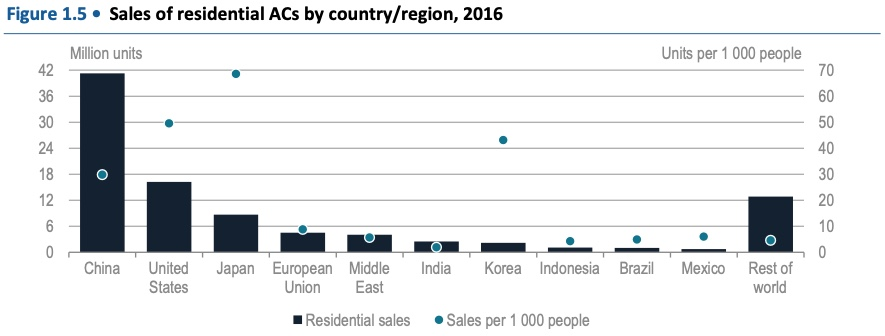
\includegraphics[width=0.8\textwidth]{Chapters/Figures/Sales of Residential ACs by Country or Region, 2016.jpg}
  \caption[Sales of Residential ACs by Country or Region, 2016]{Sales of Residential ACs by Country or Region, 2016. Source: \cite{international_energy_agency_future_2018}.}
  \label{fig:sales_acs}
\end{figure}

The growing demand for cooling is significantly influencing power systems, primarily due to the reliance on electricity-driven fans or air conditioners to meet cooling requirements. The escalating demand for air conditioning, in particular, not only elevates overall electricity consumption but also contributes to higher peak electricity loads. Additionally, the emission of greenhouse gases (GHGs) from ACs occurs through refrigerant leakage or improper disposal. It's noteworthy that these refrigerants are potent GHGs with adverse implications for climate change \cite{international_energy_agency_future_2018}. % (INTERNATIONAL ENERGY AGENCY, 2018) % rephrased

Improving the efficiency of air conditioning systems (ACs) is pivotal in mitigating peak electricity demand, thereby resulting in decreased emissions and associated financial implications. Endeavors focused on enhancing cooling efficiency necessitate a thorough assessment of the comparative costs linked to diverse cooling technologies. % rephrased

\section{Radiative Cooling}

\begin{figure}
  \centering
  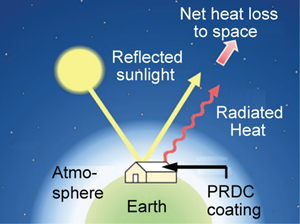
\includegraphics[width=0.4\textwidth]{Chapters/Figures/Schematic for Radiative Cooling.png}
  \caption[Schematic for Radiative Cooling] {Schematic for Radiative Cooling. Source: \cite{yang_passive_2020}}
  \label{fig:PDRC_Schematic}
\end{figure}

Objects with temperatures above absolute zero emit blackbody radiation, with a spectrum that depends on their temperature as governed by Planck's law. While the emitted radiation covers a range of wavelengths, it is not uniformly distributed across all wavelengths. Radiative passive cooling occurs when objects emit more radiation, particularly in the infrared spectrum, than the combined radiation they absorb, which includes both blackbody and solar radiation. Thus radiative passive cooling is an electricity-free method for cooling terrestrial entities \cite{yang_passive_2020}.

The heat emitted by these objects, which exceeds the heat they absorb, is transferred to outer space via thermal radiation, leveraging the substantial temperature difference between Earth (approximately 300 K) and outer space (approximately 3 K) (See figure \ref{fig:PDRC_Schematic} for net heat loss to space). This process efficiently exchanges heat with the infinite cold reservoir of deep space, achieving cooling without any energy consumption \cite{chen_passive_2022}.

Passive radiative cooling can be realized even during the daytime, necessitating precise tuning of optical properties across a broad spectrum of wavelengths, from ultraviolet to mid-infrared (see figure \ref{fig:ideal_PDRC_properties}). As a result, achieving effective passive daytime radiative cooling imposes stringent requirements on materials and structures to mitigate solar heating \cite{yang_passive_2020}:

\begin{enumerate} 
\item Minimal absorptivity ($\alpha$) approaching 0\% (equivalent to nearly 100\% reflectance, $R$) in the solar spectrum, ranging from 0.3–2.5 $\mu m$. This characteristic ensures that the surface absorbs minimal solar energy during daylight, thereby reducing the heat gained by the PDRC.
\item High thermal radiation in the atmospheric transparency window, with an emittance ($\varepsilon$) close to 1 within the long-wavelength infrared (LWIR) transmission window of the atmosphere ($\lambda$ = 8–13 $\mu m$). This range is significant due to the atmosphere's partial transparency and minimal infrared absorption by gas molecules in this spectrum.
\item An emittance ($\varepsilon$) close to 0 in other mid-infrared wavelengths, such as 5–8 $\mu m$ and those greater than 13 $\mu m$. This characteristic is crucial due to the atmosphere's opacity in these spectral ranges.
\end{enumerate}

% NB: Using [ht!] tells LaTeX to try to place the figure here, but if that's not possible, then at the top of the page, and the ! overrides LaTeX's internal parameters for deciding on figure placements. This gives you the best chance of having the figure appear right after your enumerated list, although it's not a guarantee because LaTeX might still decide to move the figure based on its page layout algorithms.
\begin{figure}[ht!]
  \centering
  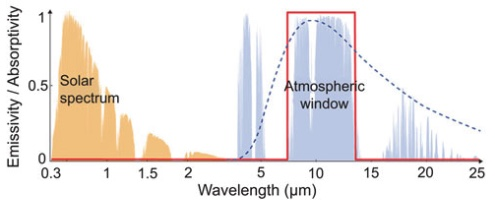
\includegraphics[width=0.4\textwidth]{Chapters/Figures/Ideal Optical Properties of a Radiative Cooling Surface.jpg}
  \caption[Ideal Optical Properties of a Radiative Cooling Surface]{Ideal Optical Properties of a Radiative Cooling Surface. Source: \cite{yang_passive_2020}}
  \label{fig:ideal_PDRC_properties}
\end{figure}


% -- SECTION 1.3: LITERATURE REVIEW ---

\section{Literature Review}
At the nexus of physics and technological advancement, Passive Daytime Radiative Cooling Devices (PDRCs) stand as a symbol of optimism amidst the challenges of global warming and the energy crisis. PDRCs are notable not just for their operational efficiency but also for their capacity to transform our approach to energy consumption and environmental conservation. While radiative cooling for nighttime use was established decades ago, only recently has there been significant progress in achieving cooling directly under sunlight, suggesting a promising upward trajectory for the technology's cooling capabilities.

The concept of radiative cooling, hypothesized by French Engineer Félix Trombe in 1965, initially focused on nighttime cooling. Significant strides have recently been made in achieving daytime cooling under direct sunlight, marking a pivotal advancement in the field. Trombe's collaboration at Montlouis Laboratory led to a cooling method that significantly reduced temperatures without insulation, leveraging a system that could cool by 14 to 30 degrees Celsius relative to the surroundings. This system involved a north-facing, slightly tilted facade with infrared-transparent panels and a selective radiator, optimizing both night and daytime cooling. % TROMBE % FORTIN

Building on Trombe's groundbreaking efforts, in 1975, Catalanotti and his team developed an experimental setup for daytime radiative cooling. This setup combined metals and TEDLAR (polyvinyl-fluoride plastic) to protect the cooling device from direct sunlight, although it was more effective for nighttime use. Further research explored the potential of thin films on aluminum substrates, with specific material compositions, such as coated thin solid film on an aluminum substrate with $\text{SiO}_6\text{N}_{0.2}$ and double layers of $\text{SiO}_2$ and $\text{SiO}_{0.25}\text{N}_{1.52}$, aimed at achieving selective emission. Despite these innovative approaches, effectively cooling during daylight remained a challenge. Catalanotti and his team, along with Bartoli and his colleagues, employed TEDLAR, a commercially available polyvinyl-fluoride polymer film, as a radiative emitter. This film, offering somewhat selective and high infrared (IR) absorption within the 9 to 13 $\mu m$ wavelength range, also absorbs IR significantly beyond 20 $\mu m$, impacting its selectivity and, consequently, the efficiency of radiative cooling. Despite this, they achieved a temperature decrease of 10 degrees Celsius below ambient under diffused sunlight. However, the primary drawback of using PVF polymer for daytime cooling is its substantial absorption in the solar spectrum.
% BIJARNIYA % [5]=The radiative cooling of selective surfaces % [6]=Materials for radiative cooling to low temperature % [7]=Surface coatings for radiative cooling applications: Silicon dioxide and silicon nitride made by reactive rf-sputtering

Ongoing advancements have aimed to enhance the cooling capabilities of radiative emitters, achieving notable success in nocturnal cooling. Yet, the reliance on both naturally sourced and synthetic polymers has imposed constraints. The absence of materials that combine high solar reflectivity with potent IR emission has hindered effective cooling under direct sunlight. Investigations into selective IR emitters, including polymer films, white pigmented paints, and SiO films, have encountered limitations due to their inadequate emissivity and the wide range of their IR absorption, which absorbs too much atmospheric radiation, thus failing to significantly lower temperatures below ambient conditions. % HOSSAIN AND GU

Additional polymer films such as polyvinylchloride (PVC) and poly(4-methylpentene) (TPX) were evaluated for their potential in radiative cooling. However, their performance, particularly in terms of IR emissivity and selectivity within the crucial 8-13 $\mu m$ range, fell short when compared to PVF.

Furthermore, investigations into pigmented paints, inorganic compounds, and gases capable of IR emission for nighttime cooling have shown promise. Specifically, white paint containing titanium dioxide (TiO$_2$), applied to aluminum plates, demonstrated notable cooling effects under clear sky conditions at night, despite less effectiveness under direct midday sun. This suggests pigmented paints might offer advantages for nocturnal cooling due to their application versatility on different substrates.

The application of Silicon Dioxide (SiO) films and other inorganic materials in radiative cooling technologies leverages their capacity for targeted infrared (IR) emission. These substances are recognized for their potential to efficiently radiate heat from surfaces, aiding in cooling processes. Nevertheless, their effectiveness is somewhat diminished by a narrow emission bandwidth, limiting the spectrum of IR radiation they can emit. This constraint may decrease the volume of heat dispersed into the environment, thereby affecting the device's cooling efficacy.

Investigations into solar reflectors and IR-transparent materials for daytime cooling have proven effective in both reflecting solar radiation and facilitating IR emission. This capability is essential for daytime cooling to both prevent solar heat accumulation and promote surface heat release. However, maintaining this delicate balance during peak sunlight, when solar irradiance is most intense, presents a considerable challenge. Achieving the optimal mix of solar reflection to avoid overheating while ensuring adequate IR emission for cooling under direct sunlight is particularly complex.

Beyond solar reflectors, convection shields significantly enhance a radiative cooler's effectiveness. In daytime operations, when a cooler's net radiative output exceeds its solar absorption, it can significantly lower temperatures beneath the ambient level, assuming convective heat gains are minimized. However, employing convection shields might not always be beneficial, as natural convection can help dissipate heat from the device. Yet, without direct sunlight, convection shields can markedly boost cooling efficiency to its maximum potential.

The advancement in photonic-based radiative coolers represents a significant leap towards achieving efficient cooling directly under sunlight, allowing temperatures to fall below ambient levels. This innovative approach differs from traditional methods that rely on the natural optical characteristics of materials, as it harnesses engineered photonic properties in tandem with those natural characteristics to enhance cooling performance.

Raman and colleagues conducted the inaugural experiment showcasing radiative cooling under direct sunlight with planar photonic structures, achieving a notable 4.9°C drop below ambient temperature. Their device, composed of seven layers alternating between hafnium oxide (HfO2) and silicon dioxide (SiO2) of varied thicknesses, utilized the upper thick layers for IR emission across the 8–13 $\mu m$ range. The lower, thinner layers on an aluminum-coated silicon wafer acted as a chirped 1D photonic crystal, reflecting up to 97\% of solar radiation.
% TODO: Attach figure 5 (a) in the Hossaini and Gu paper.
% B. BARTOLI, S. Catalanotti, B. Coluzzi, V. Cuomo, V. Silvestrini, G. Troise, Appl. Energy 1977, 3, 267.


% -- SECTION 1.4: PREVIOUS PROJECT WORK AND PROJECT GOALS ---

\section{Previous Project Work and Project Goals}
Research on PDRCs has been an ongoing project in the Hudgings lab. This thesis aims to build upon the work of Paul McKinley (class of 2022) and Genevieve diBari (class of 2023).

McKinley laid the groundwork by developing a rooftop testbed and the fabrication process for PDRCs (a process I plan to replicate after completing the modeling of various PDRC iterations on COMSOL). DiBari contributed by modeling PDRCs in Python and enhancing the initial outdoor testing setup.

For my thesis, the goal is to model different PDRC structures using COMSOL, exploring materials that could enhance the optical properties of an ideal PDRC device. This includes stacking materials of varying thicknesses and refractive indices on current PDRC models in the Hudgings lab to increase reflectivity ($R$). If time permits, promising PDRC models (with high $R$ and/or emissivity in the atmospheric window) will be fabricated after the modeling phase.


\chapter{The Physics Behind PDRCs}
A Passive Daytime Radiative Cooling (PDRC) device operates by absorbing a lower amount of blackbody radiation than it emits, thereby facilitating electricity-free cooling, even in daylight conditions. Consequently, one of the pivotal attributes of a PDRC device is the imperative for an absorptivity ($\alpha$) as close to 0\% or, conversely, a reflectivity ($R$) of 100\% within the solar spectrum (ranging from 0.3 to 2.5 micrometers). This specification ensures that the device's surface remains entirely unaffected by solar heating during daylight hours.

To enhance the effectiveness of PDRC, it becomes essential to accurately measure and optimize this reflectivity ($R$) within the solar spectrum. One approach for achieving this goal is to perceive light as an electromagnetic wave, and from this perspective, derive a quantifiable means to measure $R$ through the renowned \textit{Fresnel equations}.

The Fresnel equations are mathematical expressions that delineate the proportion of incident energy that is either transmitted or reflected at the interface of two materials with differing refractive indices. This concept aligns precisely with our objectives, as we plan to stack plane surfaces featuring distinct reflective properties and refractive indices. This chapter serves as an exploration of the theoretical framework underpinning the derivation of $R$ via the Fresnel Equations, delving into associated phenomena such as total internal reflection. Additionally, we explore the practical application of these principles to PDRC devices.


\section{Fresnel Equations}
Consider a light ray incident at point P upon a planar interface, leading to the generation of both reflected and refracted rays. It is noteworthy that the refractive index at the interface for both the incident and reflected rays ($n_1$) differs from the refractive index associated with the refracted ray ($n_2$). The plane of incidence lies within the x-z plane and is defined by both the surface normal and the incident ray.

In the context of each ray, the direction of wave propagation ($\vec{\mathbf{k}}$), can be established by the vector cross product of the electric field ($\vec{\mathbf{E}}$), and magnetic field ($\vec{\mathbf{B}}$) vectors, expressed as $\vec{\mathbf{E}} \times \vec{\mathbf{B}}$. This relationship can be conveniently determined using the right-hand rule, offering a valuable method for directional assessment.

% inserting the TE wave example
\begin{figure}
  \centering
  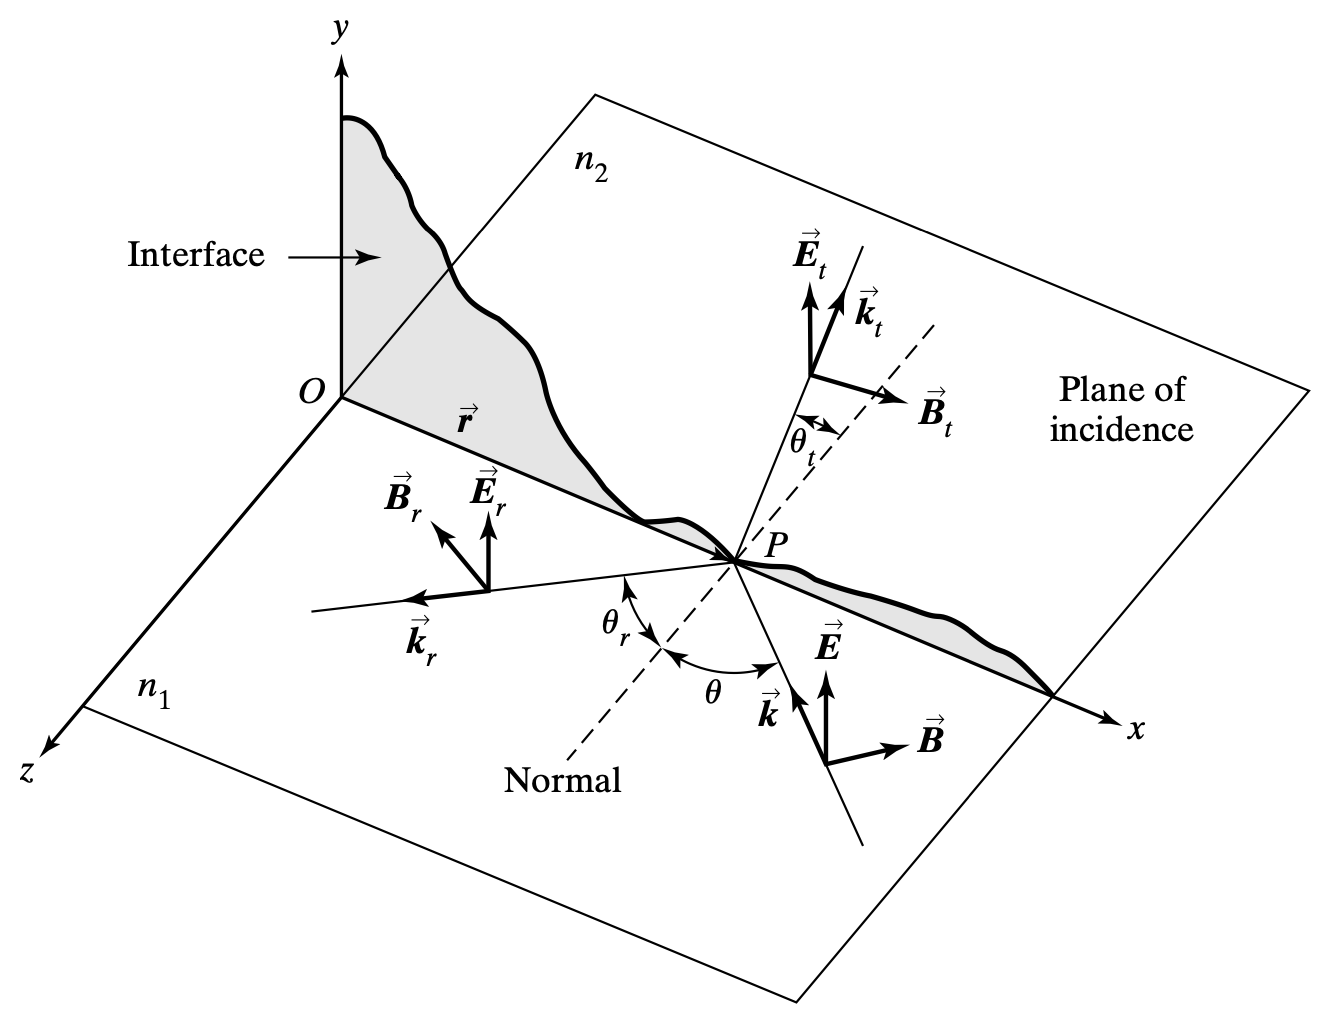
\includegraphics[width=0.8\textwidth]{Chapters/Figures/Incident, Relfected, and Transmitted Ray for TE Mode.png}
  \caption{The transverse electric (TE) set-up}
\end{figure}

Let us consider that the incident light comprises of plane harmonic waves:
\begin{equation} \label{Plane harmonic wave equation - incident}
\vec{\mathbf{E}} = \vec{\mathbf{E}_0} e^{i(\vec{\mathbf{k}} \cdot \vec{\mathbf{r}} - \omega t)}
\end{equation}
In our analytical approach, we will specifically examine a linearly polarized light wave, where the electric field vector $\vec{\mathbf{E}}$ is oriented perpendicular to the plane of incidence. According to the right-hand rule, this configuration places the magnetic field vector $\vec{\mathbf{B}}$ within the plane of incidence. This particular polarization is known as the \textit{transverse electric} (TE) mode

The reflected and transmitted waves can then also be expressed as plane harmonic wave equations:
\begin{equation} \label{Plane harmonic wave equation - reflected}
\vec{\mathbf{E}_r} = \vec{\mathbf{E}_{0r}} e^{i(\vec{\mathbf{k_r}} \cdot \vec{\mathbf{r}} - \omega_r t)}
\end{equation}

\begin{equation} \label{Plane harmonic wave equation - refracted}
\vec{\mathbf{E}_t} = \vec{\mathbf{E}_{0t}} e^{i(\vec{\mathbf{k_t}} \cdot \vec{\mathbf{r}} - \omega_t t)}
\end{equation}

At the interface where all three waves emerge simultaneously, a crucial boundary condition must be established to govern the relationship between their respective wave amplitudes. This boundary condition stipulates that the waves both incident upon and emerging from the plane of incidence should exhibit continuity and differentiability. This requirement is contingent upon the assumption that the interface is isotropic.

\subsection{Boundary Conditions for TE Waves}
In the context of our TM mode configuration, we can express the wave equations for the incident, reflected, and transmitted electric field components waves as follows:
\begin{align*}
\vec{\mathbf{E}_0} &= E\hat{y}           &  \vec{\mathbf{E}_{0r}} &= E_r\hat{y}               &  \vec{\mathbf{E}_{0t}} &= E_t\hat{y}
\end{align*}
where $E$, $E_r$, and $E_t$ denote the complex field amplitudes corresponding to the incident, reflected, and transmitted waves, respectively. These wave equations adhere to the boundary conditions, ensuring the continuity of electric field components parallel to the interface, as in:
\begin{equation} \label{Electric field boundary conditions for TE waves}
E + E_r = E_t
\end{equation}

By basic trigonometry and Maxwell's equations, we can find the corresponding magnetic fields to be:
\begin{align*} 
\vec{\mathbf{B}} &= (B\mathrm{cos}(\theta \hat{x}) - B\mathrm{sin}(\theta \hat{z})) e^{i(\vec{\mathbf{k}} \cdot \vec{\mathbf{r}} - \omega t)} \\
\vec{\mathbf{B}}_r &= (-B_r\mathrm{cos}(\theta_r \hat{x}) - B_r\mathrm{sin}(\theta_r \hat{z})) e^{i(\vec{\mathbf{k_r}} \cdot \vec{\mathbf{r}} - \omega t)} \\ 
\vec{\mathbf{B}}_t &= (B_t\mathrm{cos}(\theta_t \hat{x}) - B_t\mathrm{sin}(\theta_t \hat{z})) e^{i(\vec{\mathbf{k_t}} \cdot \vec{\mathbf{r}} - \omega t)}
\end{align*}

As the magnetic field vector lies transversely to the plane of incidence, adherence to the boundary conditions necessitates the connection of parallel components of the magnetic field, as defined by:
\begin{equation} \label{Magnetic field boundary conditions for TE waves}
B\mathrm{cos}(\theta) - B_r\mathrm{cos}(\theta) = B_t\mathrm{cos}(\theta_t) 
\end{equation}
Here, it's important to note that $\theta = \theta_r$ according to the law of reflection. Equations \ref{Electric field boundary conditions for TE waves} and \ref{Magnetic field boundary conditions for TE waves} stand as two pivotal equations arising from the boundary conditions for TE waves. These equations, instrumental in determining $R$, serve as a critical foundation. Nevertheless, before we delve into the calculation of $R$ through these boundary conditions, it is imperative to demonstrate the applicability of the same procedure to the transverse magnetic case.

\subsection{Boundary Conditions for TM Waves}
Another polarization mode for electromagnetic waves is known as the \textit{transverse magnetic} (TM) polarization. In this mode, the magnetic field vector is oriented perpendicular to the plane of incidence, while the electric field vector lies transverse to the plane of incidence. Within the framework of our TM mode configuration, we can formulate the wave equations governing the electric field components of the incident, reflected, and transmitted waves as follows:
\begin{align*} 
\vec{\mathbf{E}} &= (E\mathrm{cos}(\theta \hat{x}) - E\mathrm{sin}(\theta \hat{z})) e^{i(\vec{\mathbf{k}} \cdot \vec{\mathbf{r}} - \omega t)} \\
\vec{\mathbf{E}}_r &= (E_r\mathrm{cos}(\theta_r \hat{x}) + E_r\mathrm{sin}(\theta_r \hat{z})) e^{i(\vec{\mathbf{k_r}} \cdot \vec{\mathbf{r}} - \omega t)} \\ 
\vec{\mathbf{E}}_t &= (E_t\mathrm{cos}(\theta_t \hat{x}) - E_t\mathrm{sin}(\theta_t \hat{z})) e^{i(\vec{\mathbf{k_t}} \cdot \vec{\mathbf{r}} - \omega t)}
\end{align*}
Consequently, the magnetic field components can be written as:
\begin{align*}
    \vec{\mathbf{B}} &= -B\hat{y} e^{i(\vec{\mathbf{k}} \cdot \vec{\mathbf{r}} - \omega t)} \\
    \vec{\mathbf{B}}_r &= B_r\hat{y} e^{i(\vec{\mathbf{k}} \cdot \vec{\mathbf{r}} - \omega t)} \\
    \vec{\mathbf{B}}_t &= -B_t\hat{y} e^{i(\vec{\mathbf{k_t}} \cdot \vec{\mathbf{r}} - \omega t)} \\
\end{align*}

% inserting the TM wave example
\begin{figure}
  \centering
  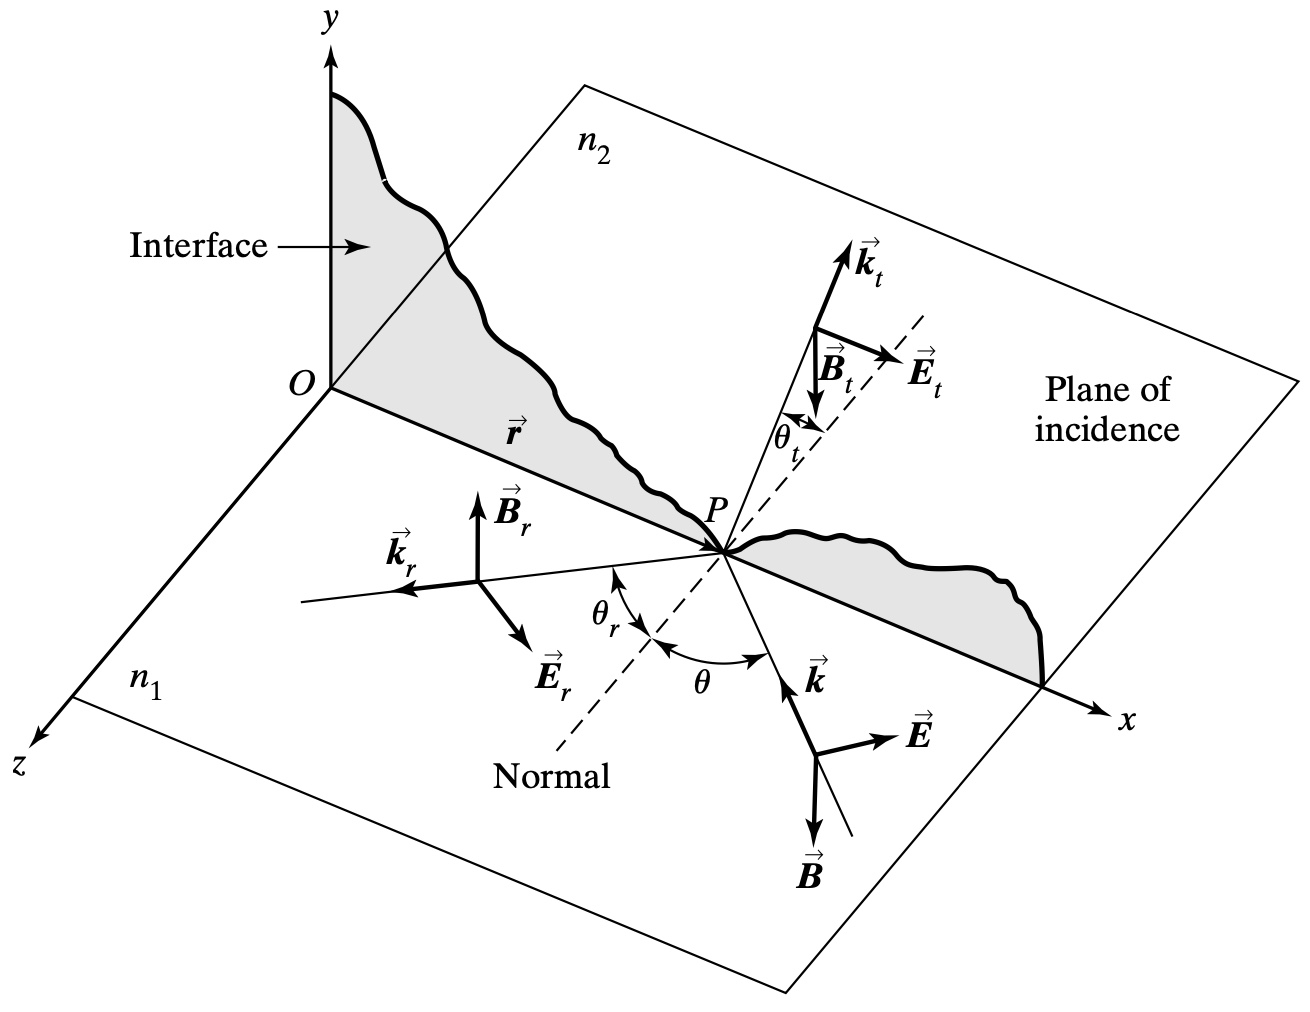
\includegraphics[width=0.8\textwidth]{Chapters/Figures/Incident, Relfected, and Transmitted Ray for TM Mode.jpg}
  \caption{The transverse electric (TM) set-up}
\end{figure}

These equations adhere to the boundary conditions, guaranteeing the continuity of electric field components parallel to the interface, as demonstrated by:
\begin{equation} \label{Magnetic field boundary conditions for TM waves}
-B + B_r = -B_t
\end{equation}

\begin{equation} \label{Electric field boundary conditions for TM waves}
Ecos(\theta) + E_rcos(\theta) = E_tcos(\theta_t)
\end{equation}

% REFLECTION AND TRANSMISSION COEFFICIENTS
\subsection{Reflection and Transmission Coefficients}
To determine the reflectance $R$ and, consequently, the transmittance $T$, it is imperative to define the reflection and transmission coefficients, as follows:
\begin{equation} \label{Definition of the reflection coefficient}
r = \frac{E_r}{E}
\end{equation}
and
\begin{equation} \label{Definition of the transmission coefficient}
t = \frac{E_t}{E}
\end{equation}

However, it is essential to calculate these coefficients for both the TE and TM cases. Recall that the electric and magnetic field amplitudes are linked through the following relation:
\begin{equation} \label{Equation relating the electric and magnetic field amplitudes}
E = \nu B = \left(\frac{c}{n}\right)B
\end{equation}

We can employ \ref{Equation relating the electric and magnetic field amplitudes} to replace every occurrence of \(B\) in the boundary conditions with its corresponding \(E\). Initiating with the TE case, remember the two vital boundary condition equations for the TE mode:
\begin{equation}
TE:
\begin{cases} \label{TE boundary conditions}
  E + E_r = E_t \\
  n_1Ecos(\theta) - n_1E_rcos(\theta) = n_2E_tcos(\theta_t)
\end{cases}
\end{equation}
We can proceed to solve the system of equations above for the TE case to determine $r_{TE}$ (by eliminating all instances of $E_t$). Introducing the concept of the \textit{relative refractive index}, denoted as $n$ and defined as $n \equiv \frac{n_2}{n_1}$, we can derive:

\begin{equation} \label{Reflection coefficient (TE) in terms of n}
r_{TE} = \frac{E_r}{E} = \frac{cos(\theta) - ncos(\theta_t)}{cos(\theta) + ncos(\theta_t)}
\end{equation}
By the law of refraction, $sin(\theta) = nsin(\theta_t)$, we can eliminate $\theta_t$ by noting that:
\begin{equation} \label{Replacing \theta_t using the law of refraction}
ncos(\theta_t) = n \sqrt{cos^{2}(\theta_t)} = n\sqrt{1 - sin^2(\theta_t)} = \sqrt{n^2 - sin^2(\theta)}
\end{equation}
Finally, our $r_{TE}$ is:
\begin{equation} \label{Reflection coefficient (TE) without \theta_t}
r_{TE} = \frac{E_r}{E} = \frac{cos(\theta) - \sqrt{n^2 - sin^2(\theta)}}{cos(\theta) + \sqrt{n^2 - sin^2(\theta)}}
\end{equation}

Likewise, employing our boundary conditions for the TM case along with \ref{Equation relating the electric and magnetic field amplitudes}, we arrive at the reevaluated boundary conditions for the TM mode, which are as follows:
\begin{equation}
TM:
\begin{cases} \label{TM boundary conditions}
  -n_1E + n_1E_r = -n_2E_t \\
  Ecos(\theta) + E_rcos(\theta) = E_tcos(\theta_t)
\end{cases}
\end{equation}
With this revised form of the boundary condition, we can compute $r_{TM}$ in a manner similar to our determination of $r_{TE}$, resulting in:
\begin{equation} \label{Reflection coefficient (TM) without \theta_t}
r_{TE} = \frac{E_r}{E} = \frac{-n^2cos(\theta) + \sqrt{n^2 - sin^2(\theta)}}{n^2cos(\theta) + \sqrt{n^2 - sin^2(\theta)}}
\end{equation}
Similarly, if we follow the same steps we did for evaluating $r_{TM}$ and $r_{TE}$, we can subsequently figure out $t_{TM}$ and $t_{TE}$ (we now eliminate $E_r$ instead of $E_t$ ). We find:
\begin{equation} \label{Reflection coefficient (TM) without \theta_t}
t_{TE} = \frac{E_t}{E} = \frac{2cos(\theta)}{cos(\theta) + \sqrt{n^2 - sin^2(\theta)}}
\end{equation}

\begin{equation} \label{Reflection coefficient (TM) without \theta_t}
t_{TM} = \frac{E_t}{E} = \frac{2ncos(\theta)}{n^2cos(\theta) + \sqrt{n^2 - sin^2(\theta)}}
\end{equation}

Observing, for instance, the interconnection between $t_{TE}$ and $r_{TE}$, it is evident that they share the same denominator, suggesting that one can be expressed in terms of the other. To establish the relationship between the two equations, one can subtract $r_{TE}$ from $t_{TE}$, yielding 1. With some additional manipulation, the corresponding equation linking $t_{TM}$ and $r_{TM}$ can be derived. Ultimately, $r$ can be expressed in terms of $t$ as follows:
\begin{align*}
    t_{TE} &= 1 + r_{TE} \\
    nt_{TM} &= 1 - r_{TM} \\
\end{align*}
The set of equations $r_{TE}$, $r_{TM}$, $t_{TE}$, and $t_{TM}$ constitutes the \textbf{Fresnel Equations}. These equations provide reflection and transmission coefficients that establish the connection between incident and reflected energy field amplitudes in any linear, isotropic, and homogeneous medium. The primary objective of the Fresnel equations is to facilitate the determination of Reflectance $R$ and Transmittance $T$, which will be discussed in the subsequent subsection.

\subsection{Reflectance and Transmittance}
For the sake of energy conservation, it is imperative that, at a specific boundary, the power incident upon the boundary equals the combined power of both the reflected and transmitted energy at that boundary.
\begin{equation} \label{power balance equation at boundary}
P_i = P_r + P_t
\end{equation}
We can preemptively define reflectance $R$ and transmittance $T$ as:
\begin{equation} \label{Reflectance}
R = \frac{P_r}{P_i}
\end{equation}
\begin{equation} \label{Transmittance}
T = \frac{P_t}{P_i}
\end{equation}
Hence, $R$ represents the proportion of reflected power relative to incident power, and transmittance $T$ signifies the proportion of transmitted power in relation to incident power. This implies that \ref{power balance equation at boundary} conforms to the well-known unity equation, under the assumption of zero absorption:
\begin{equation} \label{R+T=1}
R + T = 1
\end{equation}
Power can be defined as the product of the irradiance of the electromagnetic wave and the cross-sectional area through which the wave passes, as demonstrated by:
\begin{equation} \label{power balance equation in terms of irradiance}
I_iA_i = I_rA_r + I_tA_t
\end{equation}

To ascertain $A_i$, $A_r$, and $A_t$, it is essential to calculate the cross-sectional area covered by the incident, reflected, and transmitted electromagnetic waves, respectively. By employing trigonometric relationships, as illustrated in the accompanying figure, we can calculate the cross-sectional areas encompassed by the incident, reflected, and transmitted waves and subsequently substitute them into the equation \ref{power balance equation in terms of irradiance} to be:
\begin{equation} \label{power balance equations after CSA substitution}
I_iAcos(\theta) = I_rAcos(\theta) + I_tAcos(\theta_t)
\end{equation}

% Including the CSA example for the incident, reflected, and transmitted electromagnetic waves
\begin{figure}
  \centering
  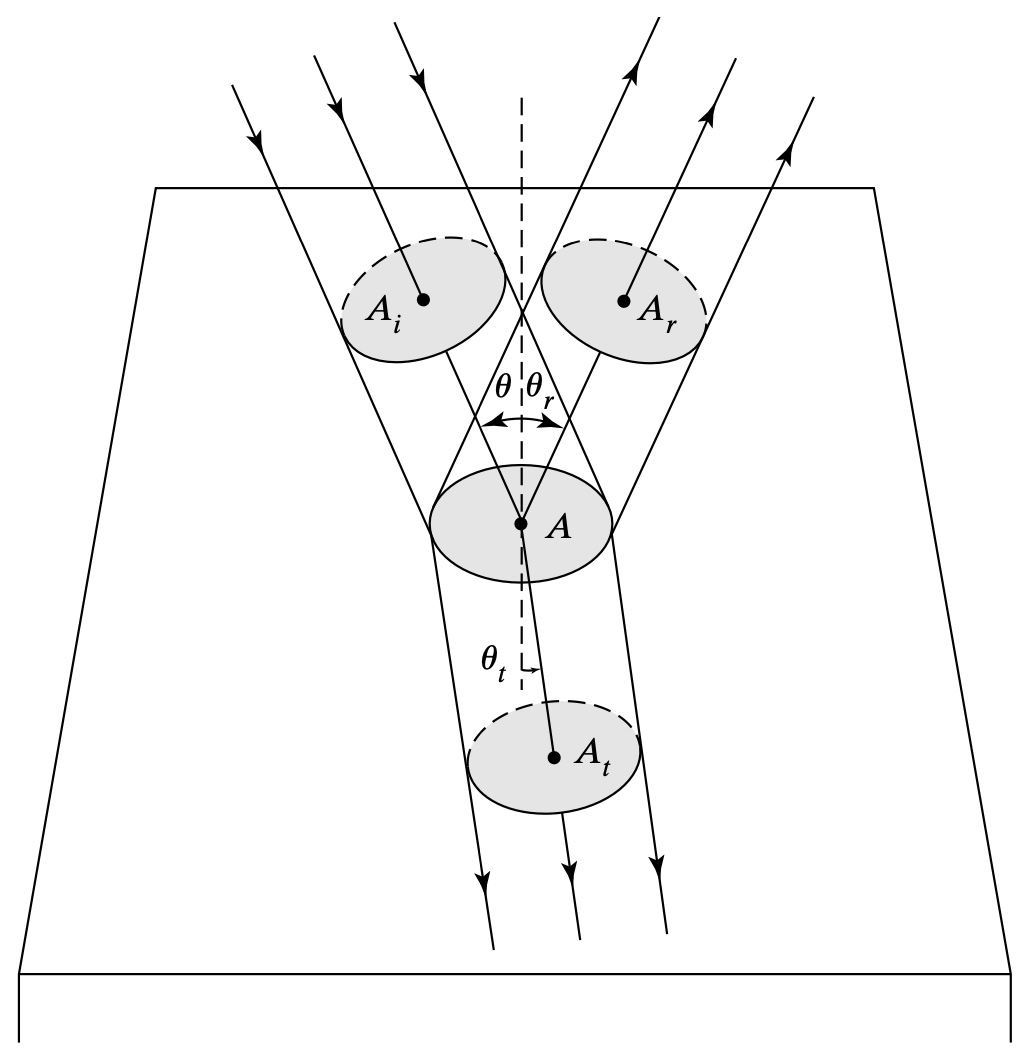
\includegraphics[width=0.8\textwidth]{Chapters/Figures/CSA Example for the Incident, Reflected, and Transmitted Electromagnetic Waves.jpg}
  \caption{Cross sections of the incident, reflected, and transmitted beams}
\end{figure}

Using the relation between irradiance and electrical field amplitude, 
\begin{equation}
I = E_{0}^2(\frac{\varepsilon \nu}{2})
\end{equation}
and that $\nu_i = \nu_r$ and $\varepsilon_i = \varepsilon_r$ since they correspond to the same medium, we can rephrase the power balance equation to be:
\begin{equation}
E_{0i}^2 = E_{0r}^2 + E_{0t}^2\left(\frac{\nu_t\varepsilon_t}{\nu_i\varepsilon_i}\right) \left(\frac{cos(\theta_t)}{cos(\theta)} \right)
\end{equation}
$\frac{\nu_t\varepsilon_t}{\nu_i\varepsilon_i}$ is a complicated way of expressing $n$ - the relative refractive index. Using the facts that $\mu_i = \mu_t = \mu_0$ (for nonmagnetic materials) and the relation that $\nu^2 = \frac{1}{\mu\varepsilon}$:
\begin{equation}
\frac{\nu_t\varepsilon_t}{\nu_i\varepsilon_i} = \frac{\nu_i^2\mu_i}{\nu_t^2\mu_t} \frac{\nu_t}{\nu_i} = \frac{\nu_i}{\nu_t} = n
\end{equation}
Thus we can include $n$ in the power balance equations:
\begin{equation}
E_{0i}^2 = E_{0r}^2 + n E_{0t}^2 \left(\frac{cos(\theta_t)}{cos(\theta)} \right)
\end{equation}
Dividing through by $E_{0i}^2$, we get:
\begin{equation} \label{power balance equation with r^2 and t^2}
1 = r^2 + n t^2 \left(\frac{cos(\theta_t)}{cos(\theta)} \right)
\end{equation}
Note that equations \ref{Definition of the reflection coefficient} and \ref{Definition of the transmission coefficient} allow us to make the substitutions for $r$ and $t$ above. Note that \ref{power balance equation with r^2 and t^2} certify that:

\begin{equation} \label{definition of R}
R = \frac{P_r}{P_i} = \frac{I_r}{I_i} = r^2
\end{equation}
Consequently,
\begin{equation} \label{definition of T}
T =  n t^2 \left(\frac{cos(\theta_t)}{cos(\theta)} \right)
\end{equation}

It's worth noting that $T$ is not merely $t^2$, as we must consider the altered speed of the electromagnetic wave when it enters a medium with a different refractive index. This change in speed impacts the rate of energy propagation and, consequently, the power of the beam.

%------------- FROM THE THEORY OF MULTILAYER FILMS ------------
\section{Multilayer films}
In the development of Passive Daytime Radiative Cooling Devices (PDRCs), we intend to employ multiple stacks comprising diverse materials with distinct refractive indices, arranged in layers to enhance the overall reflection coefficient and consequently increase reflectance. It is crucial to comprehend the electromagnetic wave interaction and optimal layer stacking physics to maximize reflectance. We again need a rigorous consideration of boundary conditions as dictated by Maxwell's equations. %R

\subsection{Transfer Matrix}
Consider the set-up above where the electric field amplitude is perpendicular to the plane of incidence (a transverse electric (TE) wave).

% inserting the multilayer film set-up
\begin{figure}
  \centering
  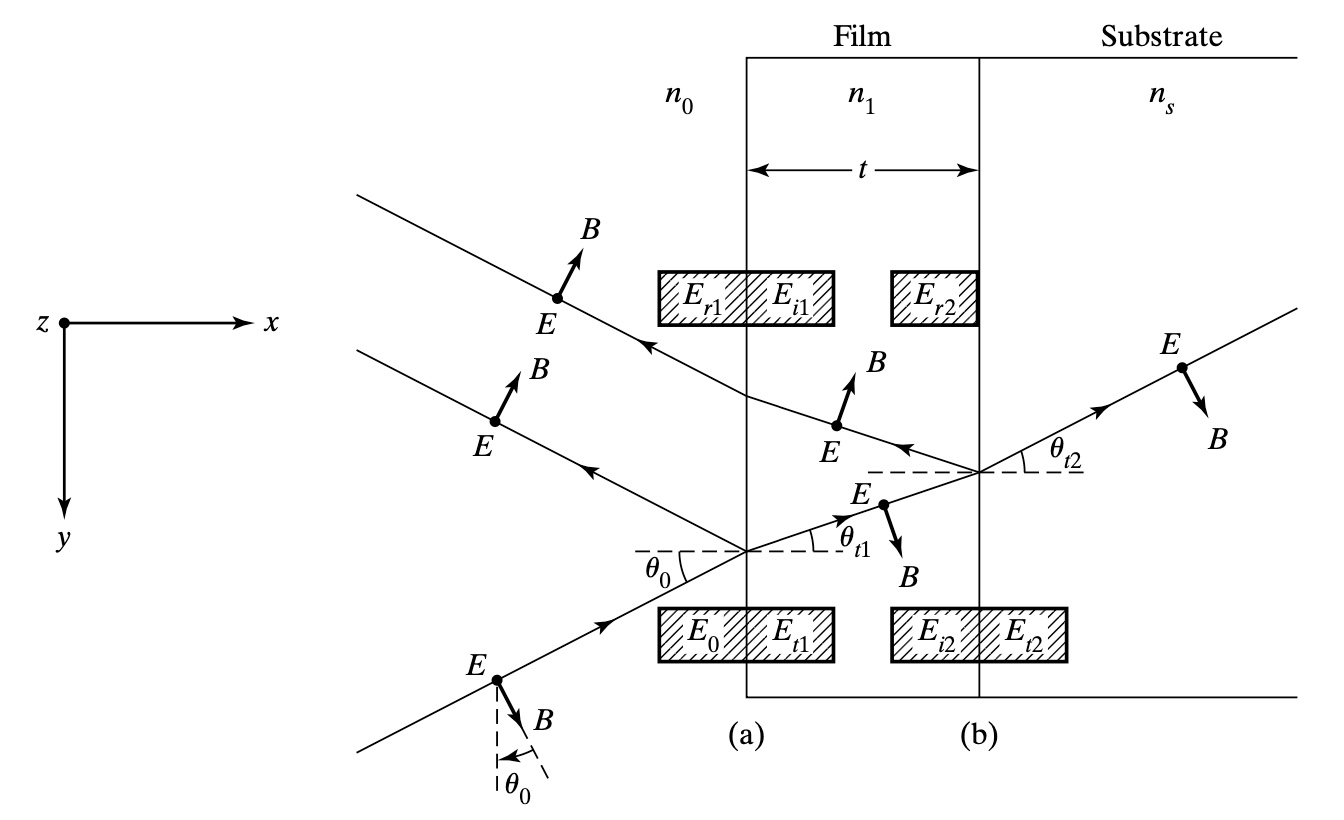
\includegraphics[width=0.8\textwidth]{Chapters/Figures/Multilayer Film Set-Up.jpeg}
  \caption{Multilayer Film Set-Up}
\end{figure}

A TE wave travels from air and makes it way to the air-film boundary. A portion of the beam is transmitted some of it is reflected. Subsequently, the transmitted beam is then incident on the film-substrate interface where a portion is further transmitted and another is reflected. This reflected bit then becomes incident on the film-air interface where some of it is transmitted and some is reflected and so on and so forth. One can imagine this at a larger scale where we could have multiple films. Notice that the film and substrate have different refractive indices, $n_1$ and $n_s$ respectively.

To capture the intricate interplay of reflected and transmitted beams, we develop a convenient notation as clearly evident on the set-up image. For example, $E_{r1}$ represents the sum of all the multiply reflected beams at interface (a). $E_{i2}$ represents the sum of all the multiple beams incident at interface (b) and going toward the substrate.

Again, we hold true to our assumptions that the film is both homogeneous (has the same properties at every point) and isotropic (the physical properties do not differ regardless of the direction or orientation in which it is examined). Moreover, we assume further that the thickness of the film is on the order of wavelength of light.

The boundary conditions for the electric and magnetic fields of plane waves, which follow from Maxwell's equation, dictate that the tangential components of the electric and magnetic fields should be continuous across the interface, that is, equal on either side. Notice that the electric field component is everywhere tangent to the interfaces but since the magnetic field vector has to be tangential to the electric field vector, we need to find the consequent tangential magnetic field vectors so that we can properly invoke the boundary conditions.

\begin{equation} \label{E_a - Multilayer films electric field boundary equations}
E_a = E_0 + E_{r1} = E_{t1} + E_{i1}
\end{equation}

\begin{equation} \label{E_b - Multilayer films electric field boundary equations}
E_b = E_{i2} + E_{r2} = E_{t2}
\end{equation}

To figure out the tangential magnetic field vectors, we can employ trigonometry to find the following boundary conditions:

\begin{equation} \label{B_a - Multilayer films magnetic field boundary equations}
B_a = B_0cos(\theta_0) - B_{r1}cos(\theta_0) = B_{t1}cos(\theta_{t1}) - B_{i1}cos(\theta_{t1})
\end{equation}

\begin{equation} \label{B_b - Multilayer films magnetic field boundary equations}
B_b = B_{i2}cos(\theta_{t1}) - B_{r2}cos(\theta_{t1}) = B_{t2}cos(\theta_{t2})
\end{equation}

We can build on equation \ref{Equation relating the electric and magnetic field amplitudes} to notice that we can express B in terms of E by doing this:
\begin{equation} \label{Alternative B and E representation}
B = n\sqrt{\varepsilon_0\mu_0}E
\end{equation}
and since $c=\frac{1}{\sqrt{\varepsilon_0\mu_0}}$, we can rewrite \ref{B_a - Multilayer films magnetic field boundary equations} and \ref{B_b - Multilayer films magnetic field boundary equations} in terms of \ref{Alternative B and E representation}.

\begin{equation} \label{Alternative B_a - Multilayer films magnetic field boundary equations}
B_a = \gamma_0(E_0 - E_{r1}) = \gamma_1(E_{t1} - E_{i1})
\end{equation}

\begin{equation} \label{Alternative B_b - Multilayer films magnetic field boundary equations}
B_b = \gamma_1(E_{i2} - E_{r2}) = \gamma_sE_{t2}
\end{equation}

\chapter{Computational Methods}
COMSOL Multiphysics\textsuperscript{TM} is a comprehensive software suite for finite element analysis, solving, and simulation across a wide array of physics and engineering disciplines, particularly focusing on coupled phenomena and multiphysics interactions. It enables the creation and simulation of physics-based models and applications in an intuitive, interactive workspace.

COMSOL software supports a broad spectrum of applications, from electromagnetics and structural mechanics to acoustics, fluid dynamics, heat transfer, and chemical engineering. COMSOL features an extensive array of modules, including the Wave Optics module for optical applications simulations like wave propagation in fiber optics and photonics, the Semiconductor module for the analysis of semiconductor devices such as diodes and transistors, and the AC/DC module for examining electric and magnetic fields in static and low-frequency scenarios. For my thesis, which involves analyzing ray paths in optical systems, I will be utilizing the Ray Optics module.

% ----- THE MODELLING WORKFLOW -----
\section{The COMSOL Modelling Workflow}
Briefly the modelling workflow consists of the following steps, if you start a model completely from scratch:

\begin{enumerate}
    \item \textbf{Initialization of the Model Environment}: Preparing the foundational settings for the simulation.
    \item \textbf{Geometry Construction}: Designing the model's physical layout.
    \item \textbf{Material Property Specification}: Assigning specific materials to the model components.
    \item \textbf{Physics Boundary Conditions Definition}: Establishing the physical constraints and conditions.
    \item \textbf{Mesh Generation}: Creating the computational grid over the model.
    \item \textbf{Simulation Execution}: Performing the actual computational analysis.
    \item \textbf{Results Post-Processing}: Analyzing and visualizing the simulation outcomes.
\end{enumerate}

In this context, I will demonstrate this workflow first through a simple project, illustrating COMSOL's robust capabilities and the straightforwardness of applying this workflow across various projects. It's important to recognize that this workflow remains consistent across different physics simulations, which will guide the development of subsequent models for my thesis.

This demonstration will focus on simulating Joule heating within a busbar, a process where electric current passing through metal results in heating due to electrical resistance.

The busbar in question will incorporate three titanium bolts, with electrical current flowing from a single bolt on one end to a pair of bolts at the opposite end. The objective is to observe the resulting temperature distribution as the busbar undergoes heating.

% Busbar image
\begin{figure}[ht!]
  \centering
  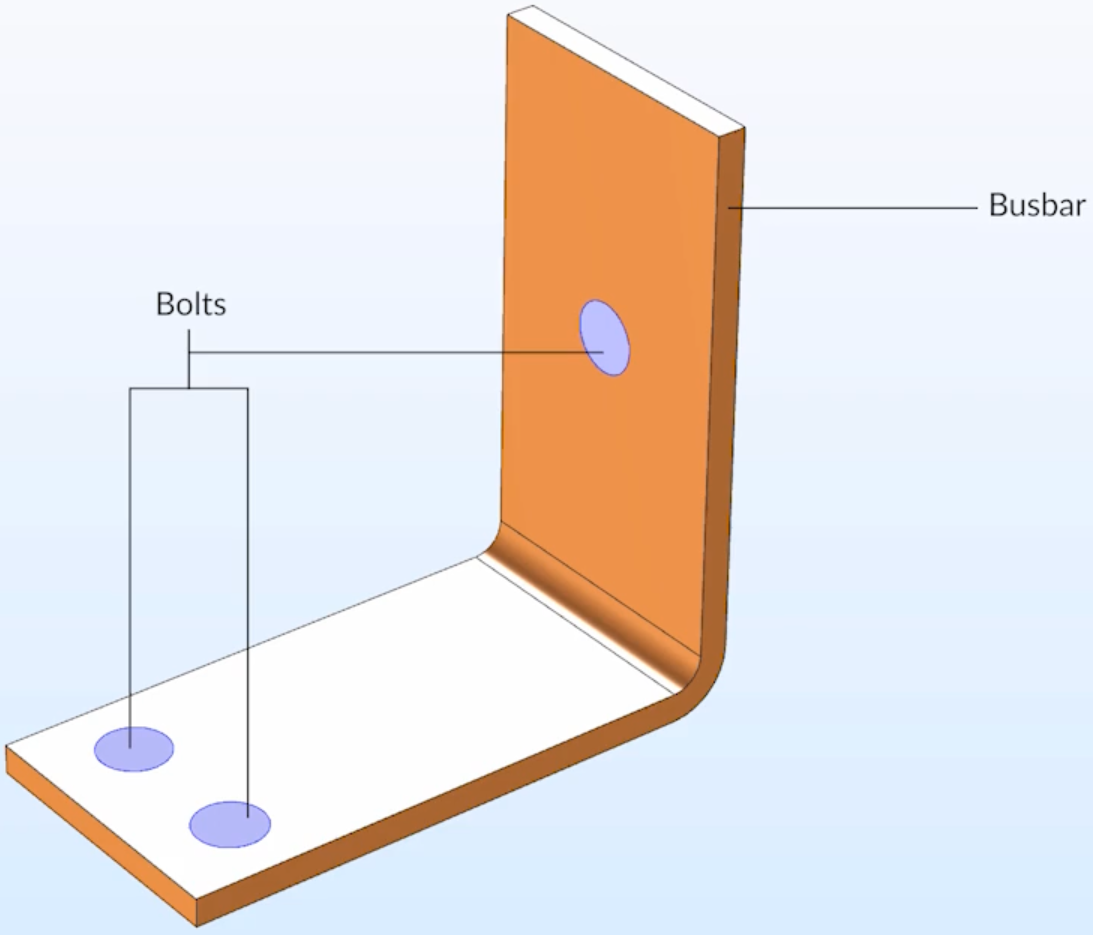
\includegraphics[width=0.4\textwidth]{Chapters/Figures/Chapter 3 Figures/Busbar.png}
  \caption{ Source: \cite{}}
  \label{}
\end{figure}

% SUBSECTION --- Setting up the model environment ---
\subsection{Setting Up the Model Environment}.
% TODO: Add set-up screen image
\begin{figure}[ht!]
  \centering
  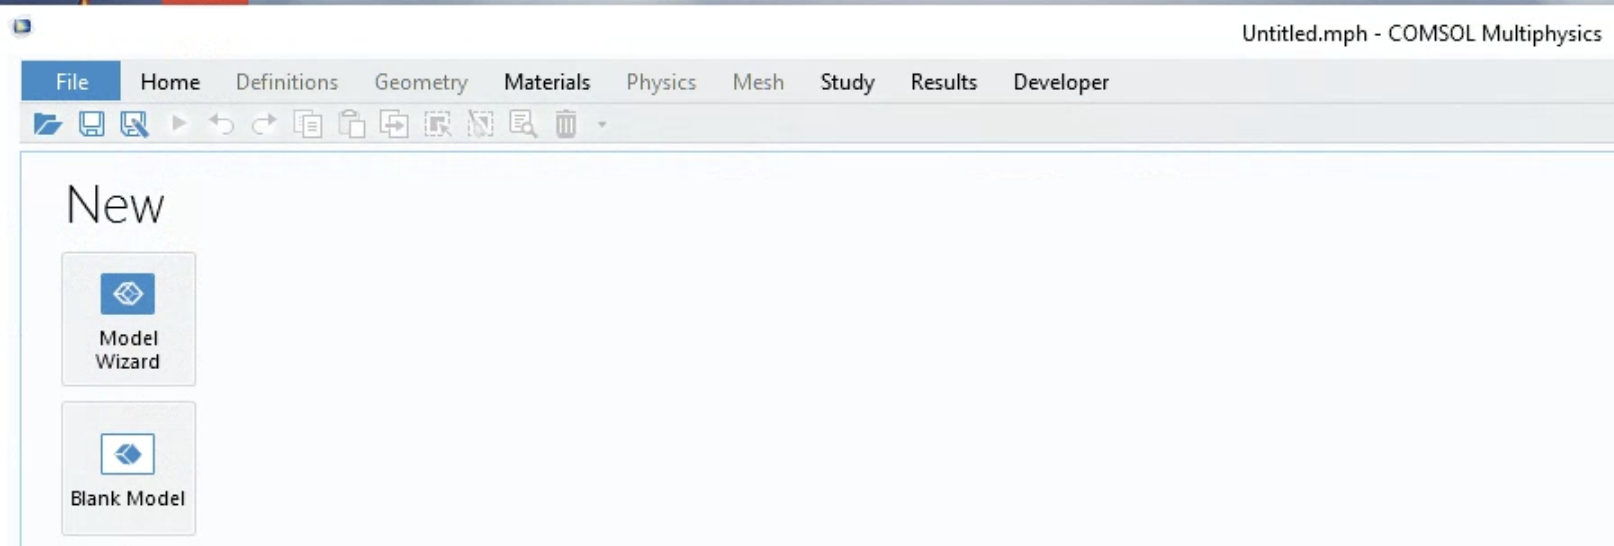
\includegraphics[width=0.4\textwidth]{Chapters/Figures/Chapter 3 Figures/Set-up Screen.png}
  \caption{ Source: \cite{}}
  \label{}
\end{figure}

Upon launching COMSOL, you are presented with an option to initiate a new project: selecting a Blank Model for starting anew or opting for the Model Wizard for a guided setup. The Model Wizard is advisable for its structured selection process integral to configuring your model. Conversely, choosing a Blank Model grants immediate access to the COMSOL desktop interface, bypassing the preliminary selections required by the Model Wizard.

% TODO: Add "Select Space Dimension" image
\begin{figure}[ht!]
  \centering
  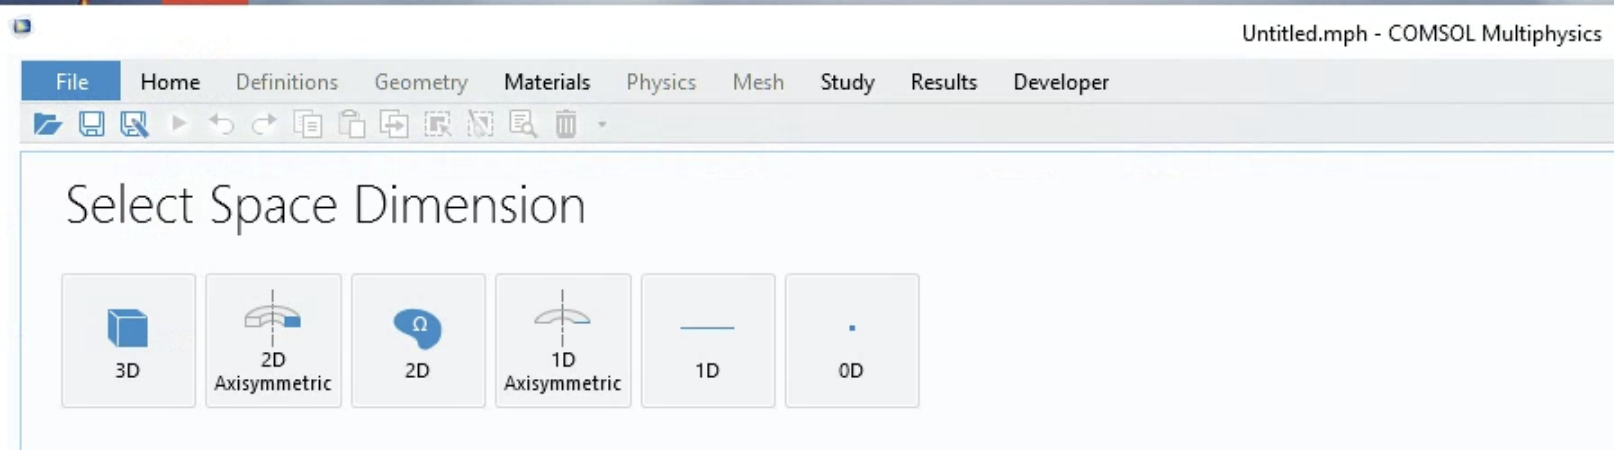
\includegraphics[width=0.4\textwidth]{Chapters/Figures/Chapter 3 Figures/Select Space Dimension.png}
  \caption{ Source: \cite{}}
  \label{}
\end{figure}

Since our busbar model requires a three-dimensional framework, we select the ``3D'' option.

% TODO: Add "Select Physics" image
\begin{figure}[ht!]
  \centering
  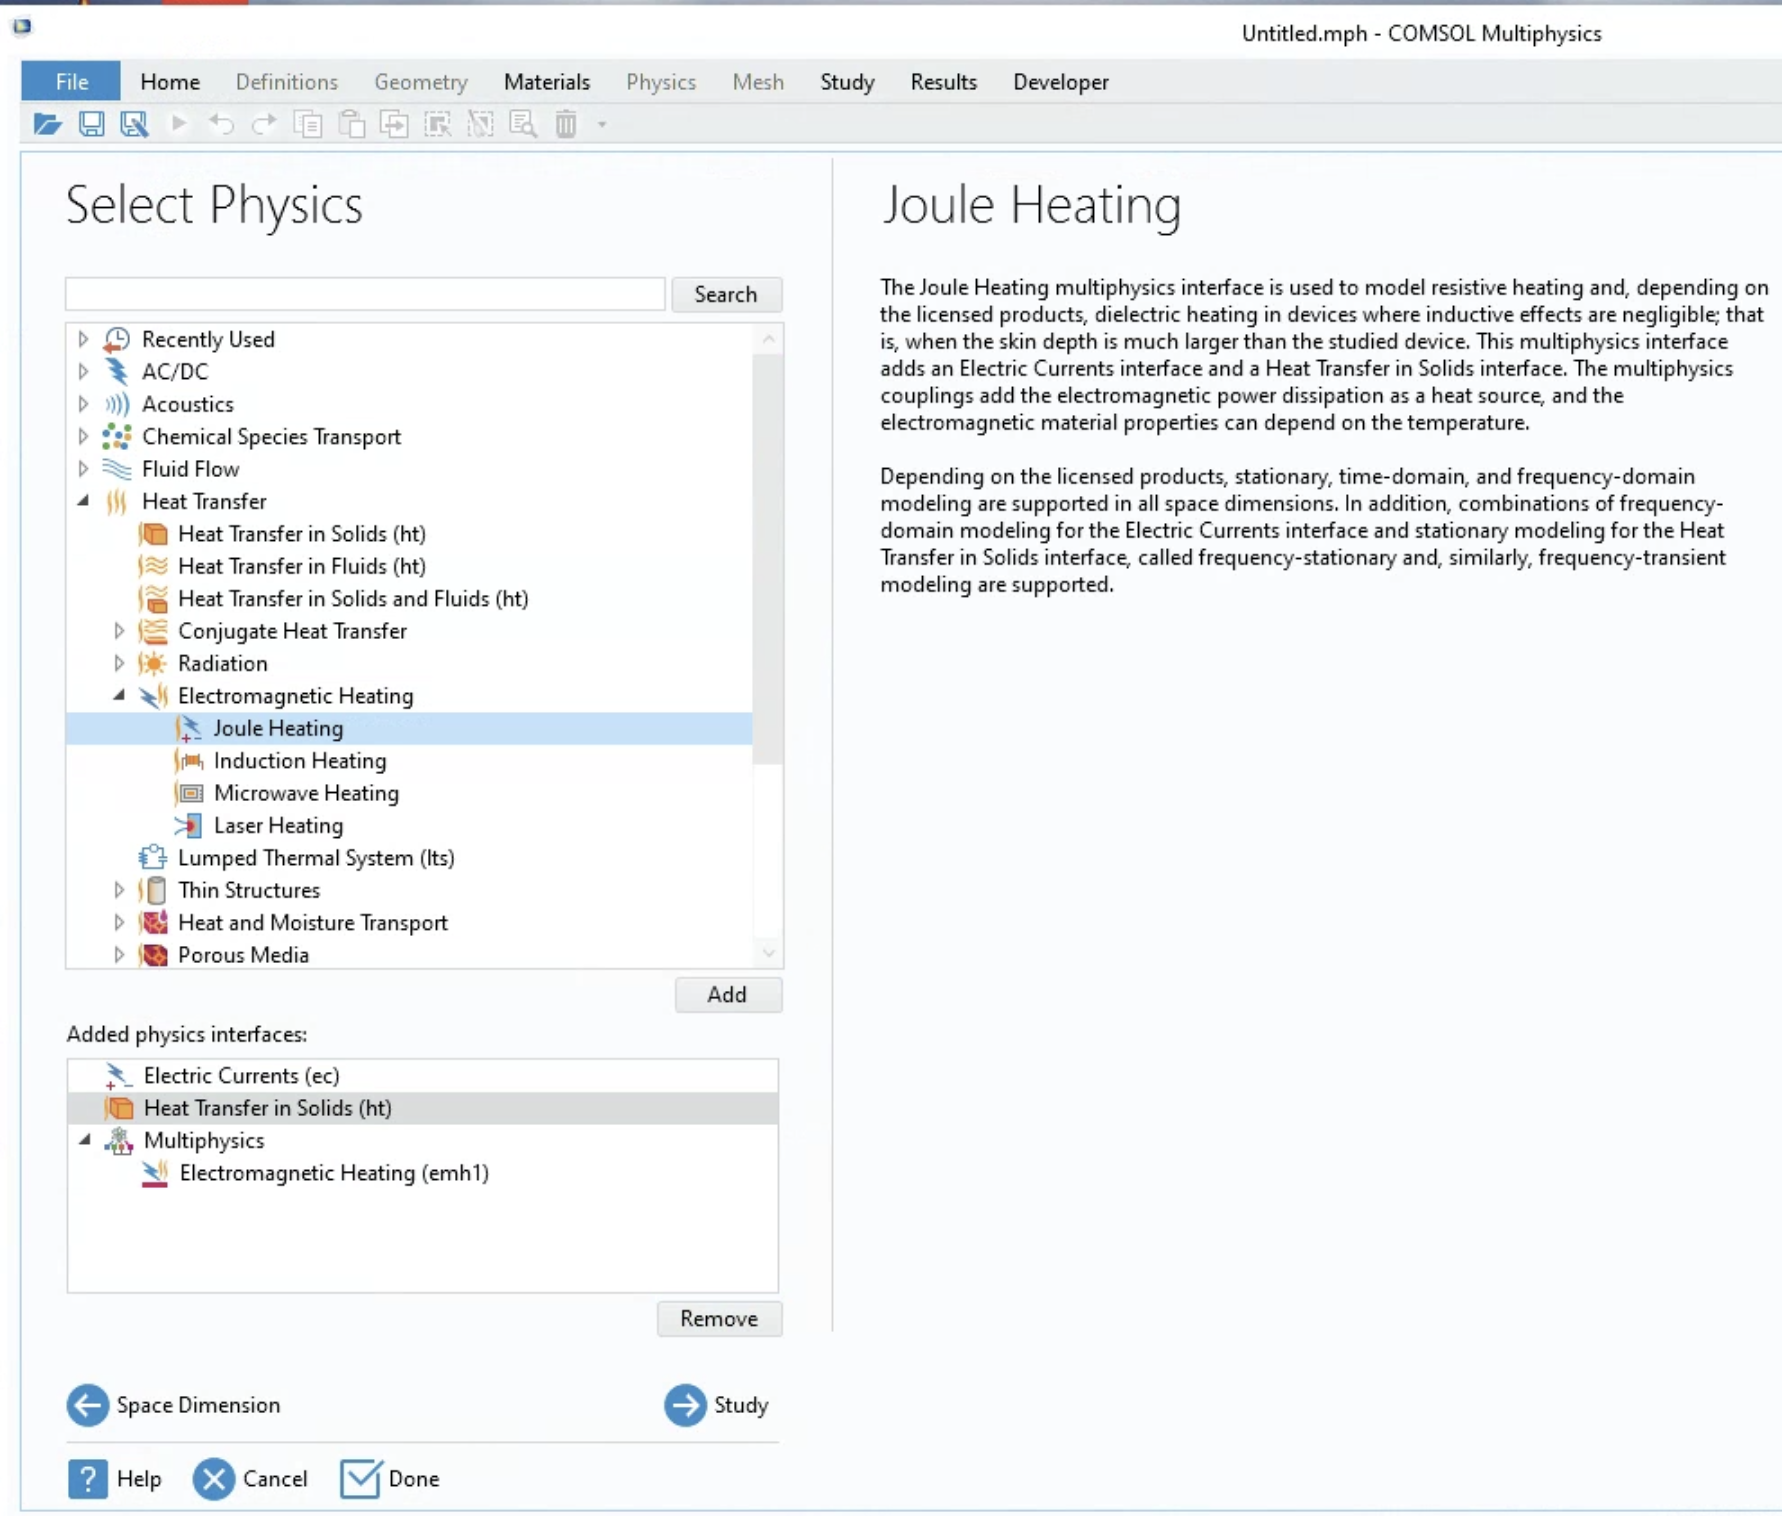
\includegraphics[width=0.4\textwidth]{Chapters/Figures/Chapter 3 Figures/Select Physics.png}
  \caption{ Source: \cite{}}
  \label{}
\end{figure}

Subsequently, we arrive at a prompt to select the desired physics for the model. In our case, we opt for Joule heating. In another scenario, for instance, if one's project was on thin-film fluid flow, navigating to the ``Fluid Flow'' node and selecting ``Thin-Film Flow'' would be the procedure. Adding ``Joule Heating'' automatically associates it with related physics categories like ``Electric Currents (ec)'' and ``Heat Transfer in Solids (ht),'' indicating that ``Joule Heating'' encompasses a composite interface with multiple physics elements integrated.

The selection of physics for exploration significantly hinges on the project's specific requirements and the level of access provided by your COMSOL subscription. For example, acquiring the ``Ray Optics'' module necessary for my thesis entailed a waiting period due to initial subscription limitations. Therefore, early verification of the required physics for your project is recommended.

To proceed, we select ``Study''.

% TODO: Add "Select Study" image
\begin{figure}[ht!]
  \centering
  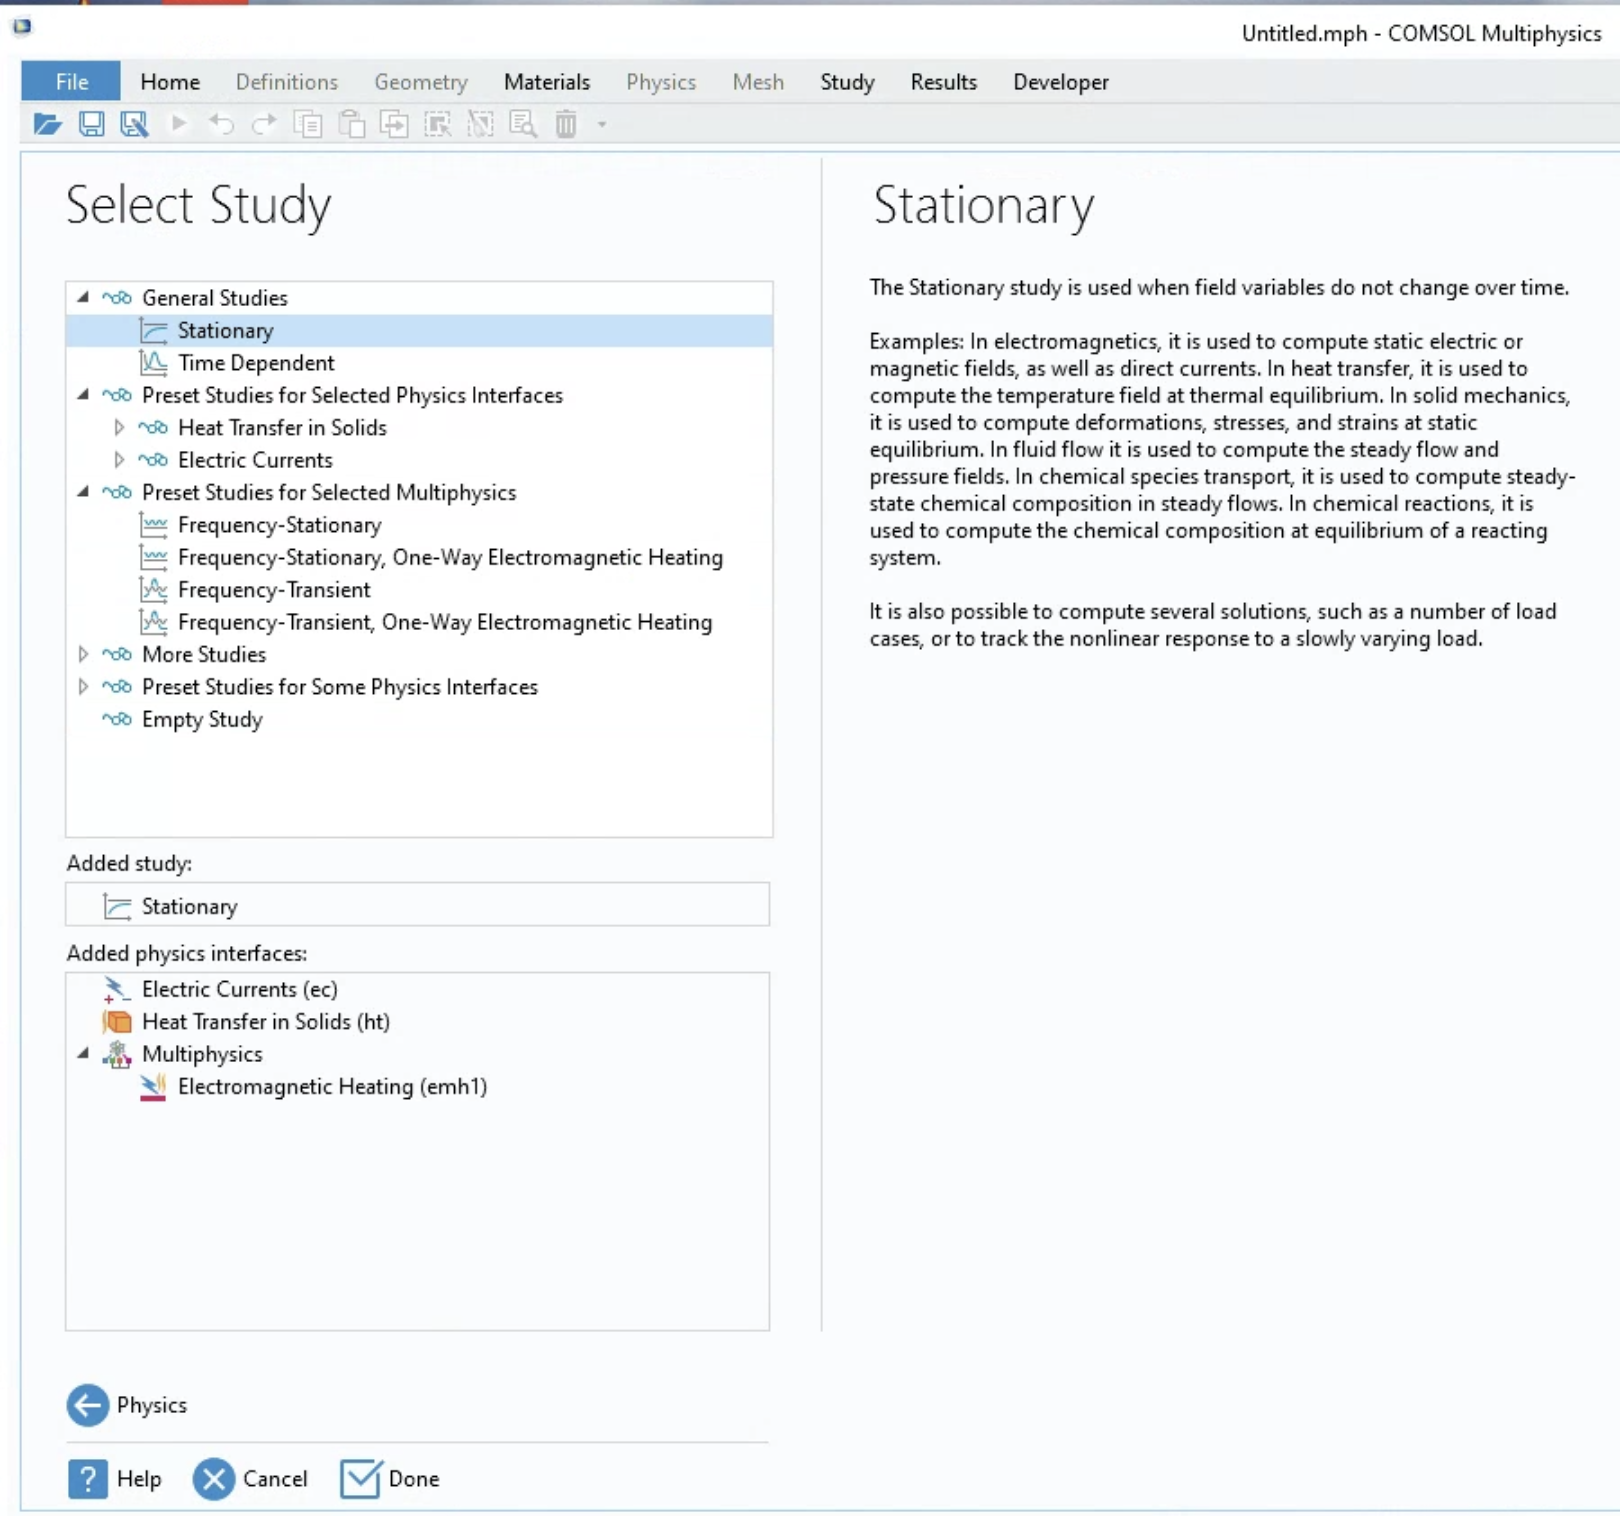
\includegraphics[width=0.4\textwidth]{Chapters/Figures/Chapter 3 Figures/Select Study.png}
  \caption{ Source: \cite{}}
  \label{}
\end{figure}

Upon accessing this interface, we are presented with an assortment of study options, determined by our earlier selections regarding the model's spatial dimensions and physics. For our busbar analysis, the ``Stationary'' study suffices, given its static nature. After selecting ``Done'', we transition to the COMSOL desktop environment.


% TODO: Add "COMSOL Desktop" image
\begin{figure}[ht!]
  \centering
  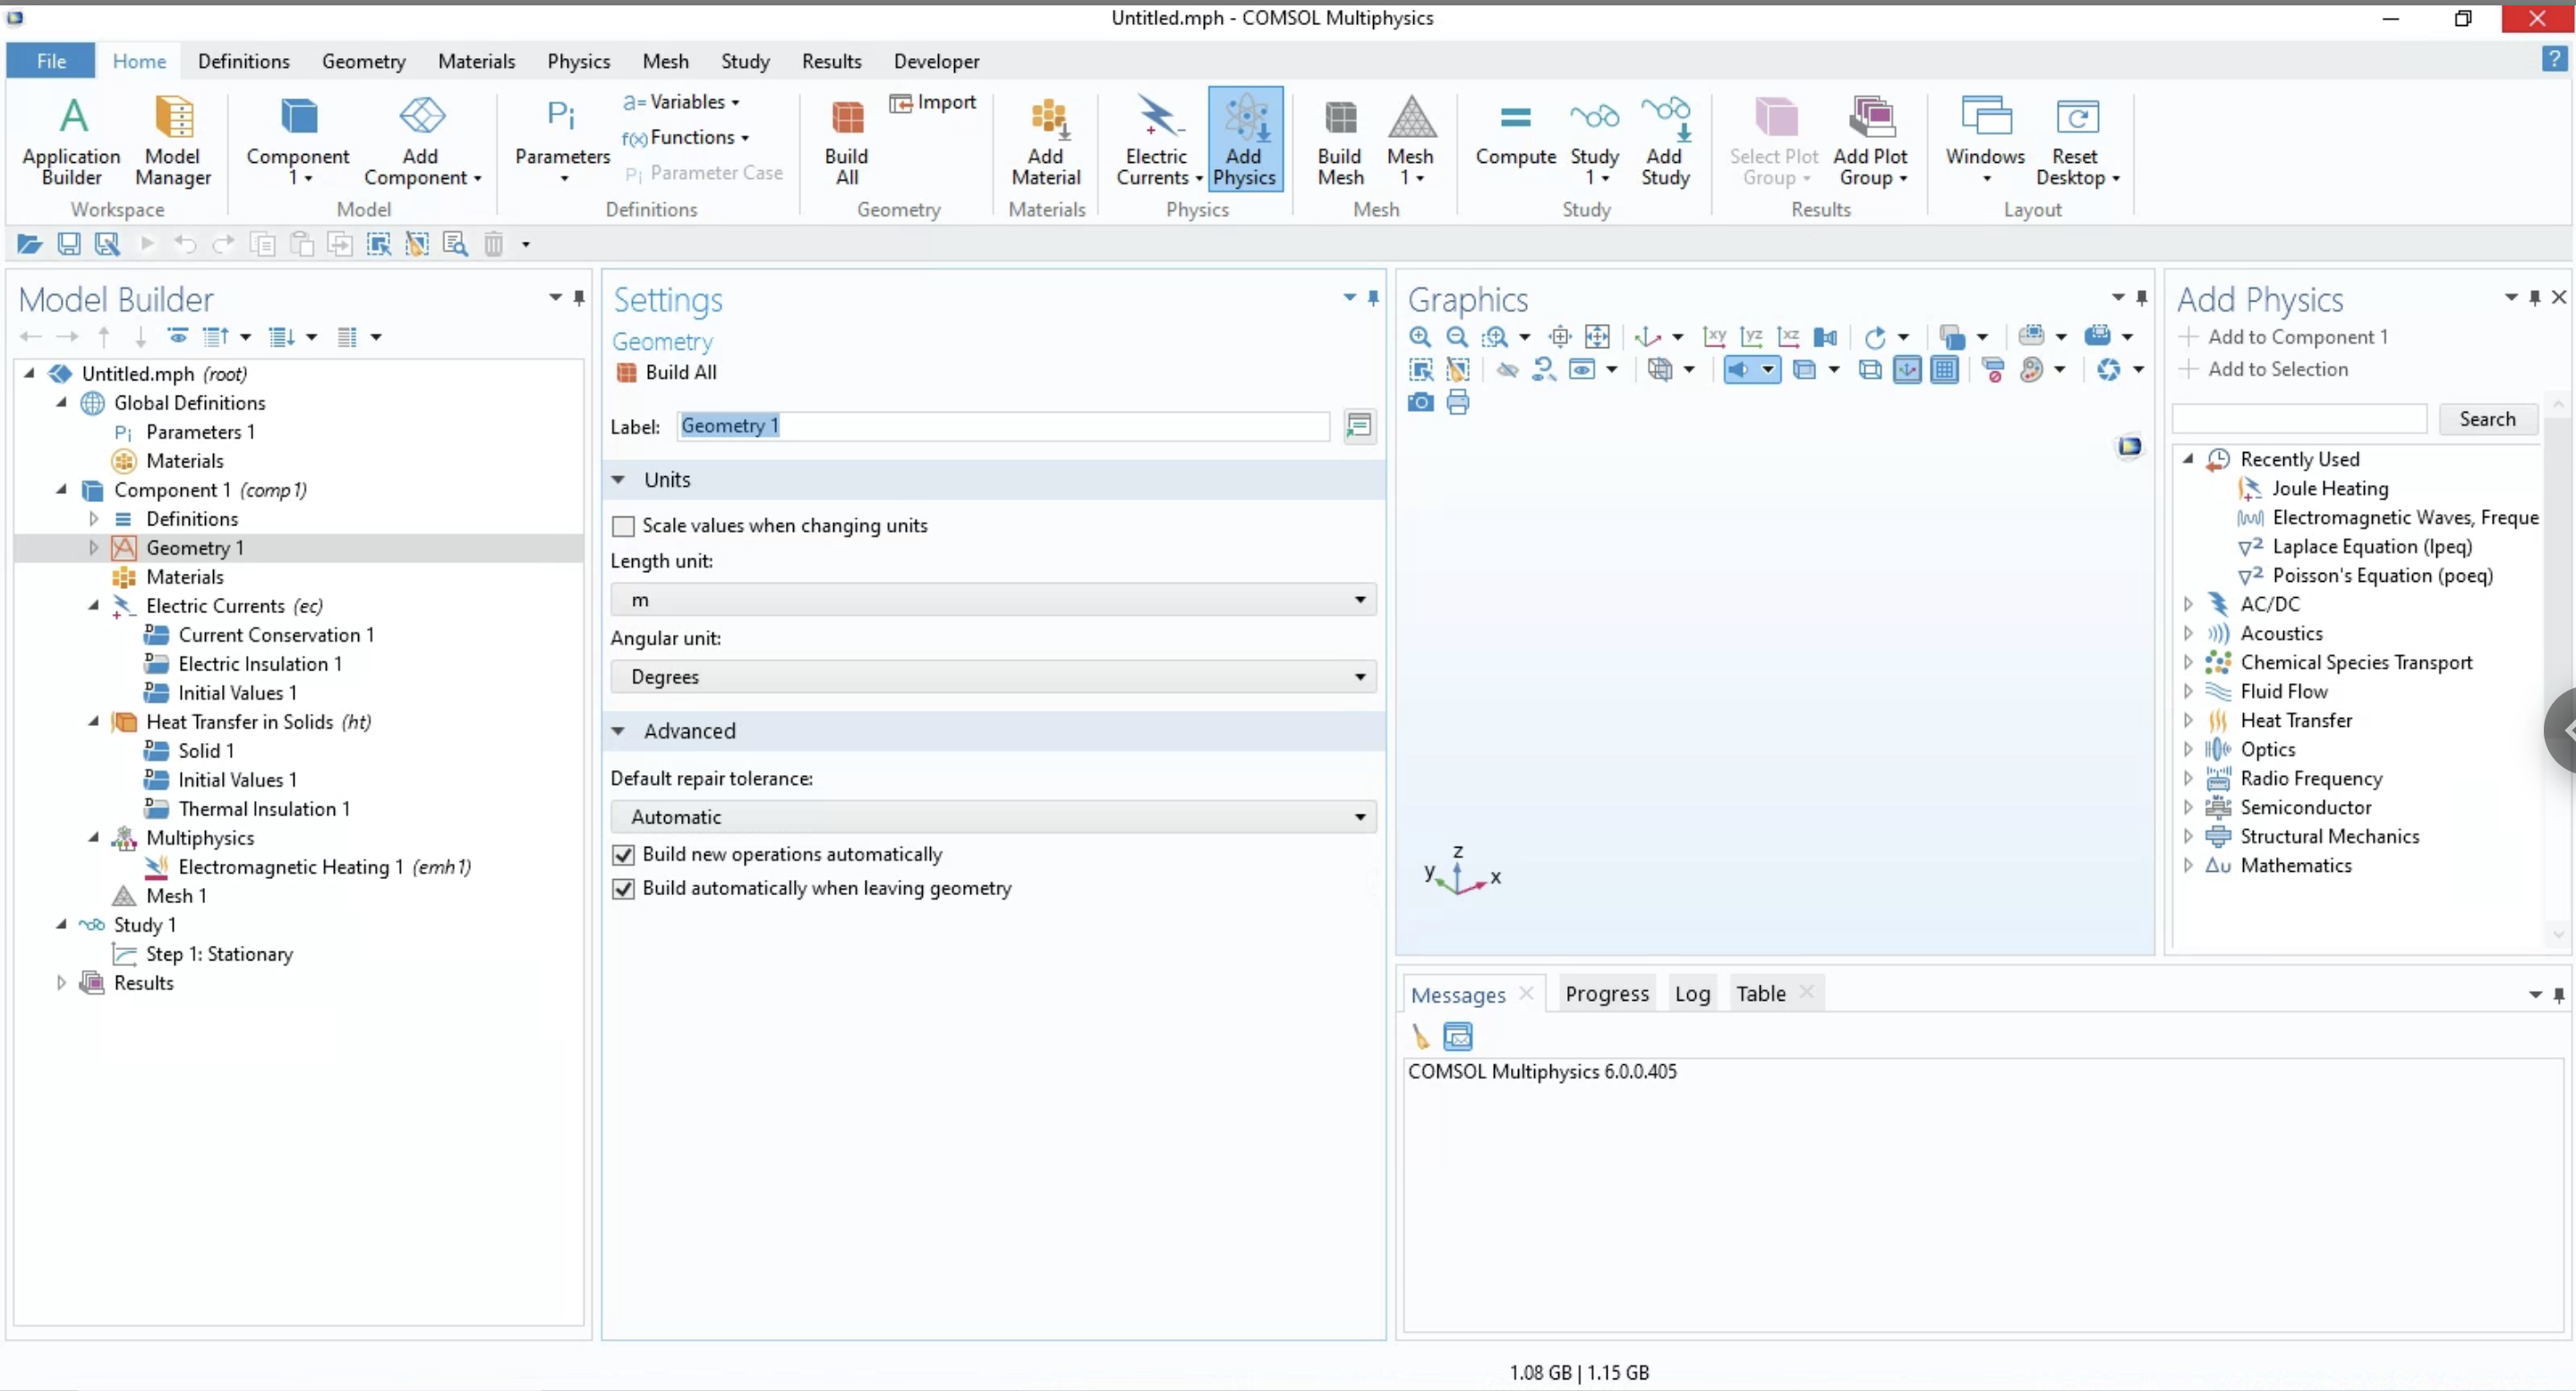
\includegraphics[width=0.4\textwidth]{Chapters/Figures/Chapter 3 Figures/Initial COMSOL Desktop.png}
  \caption{ Source: \cite{}}
  \label{}
\end{figure}

The COMSOL desktop serves as the central hub for constructing and engaging with your model from the ground up. It is designed with an intuitive interface, featuring buttons and ribbons aligned with the modeling process steps. Within the Model Builder window, you'll find the modeling hierarchy, where you have the capability to define your model's dimensions and select specific physics equations for adherence. Additionally, the layout of the COMSOL desktop windows can be customized to suit your preferences.


% SUBSECTION --- Building the Geometry ---
\subsection{Building the Geometry}.
When developing the geometry of your model, multiple pathways are available. You may opt to utilize the drawing tools or geometric shapes provided by COMSOL or import a geometry from an external source.

% TODO: Add "Geometry Button" image
\begin{figure}[ht!]
  \centering
  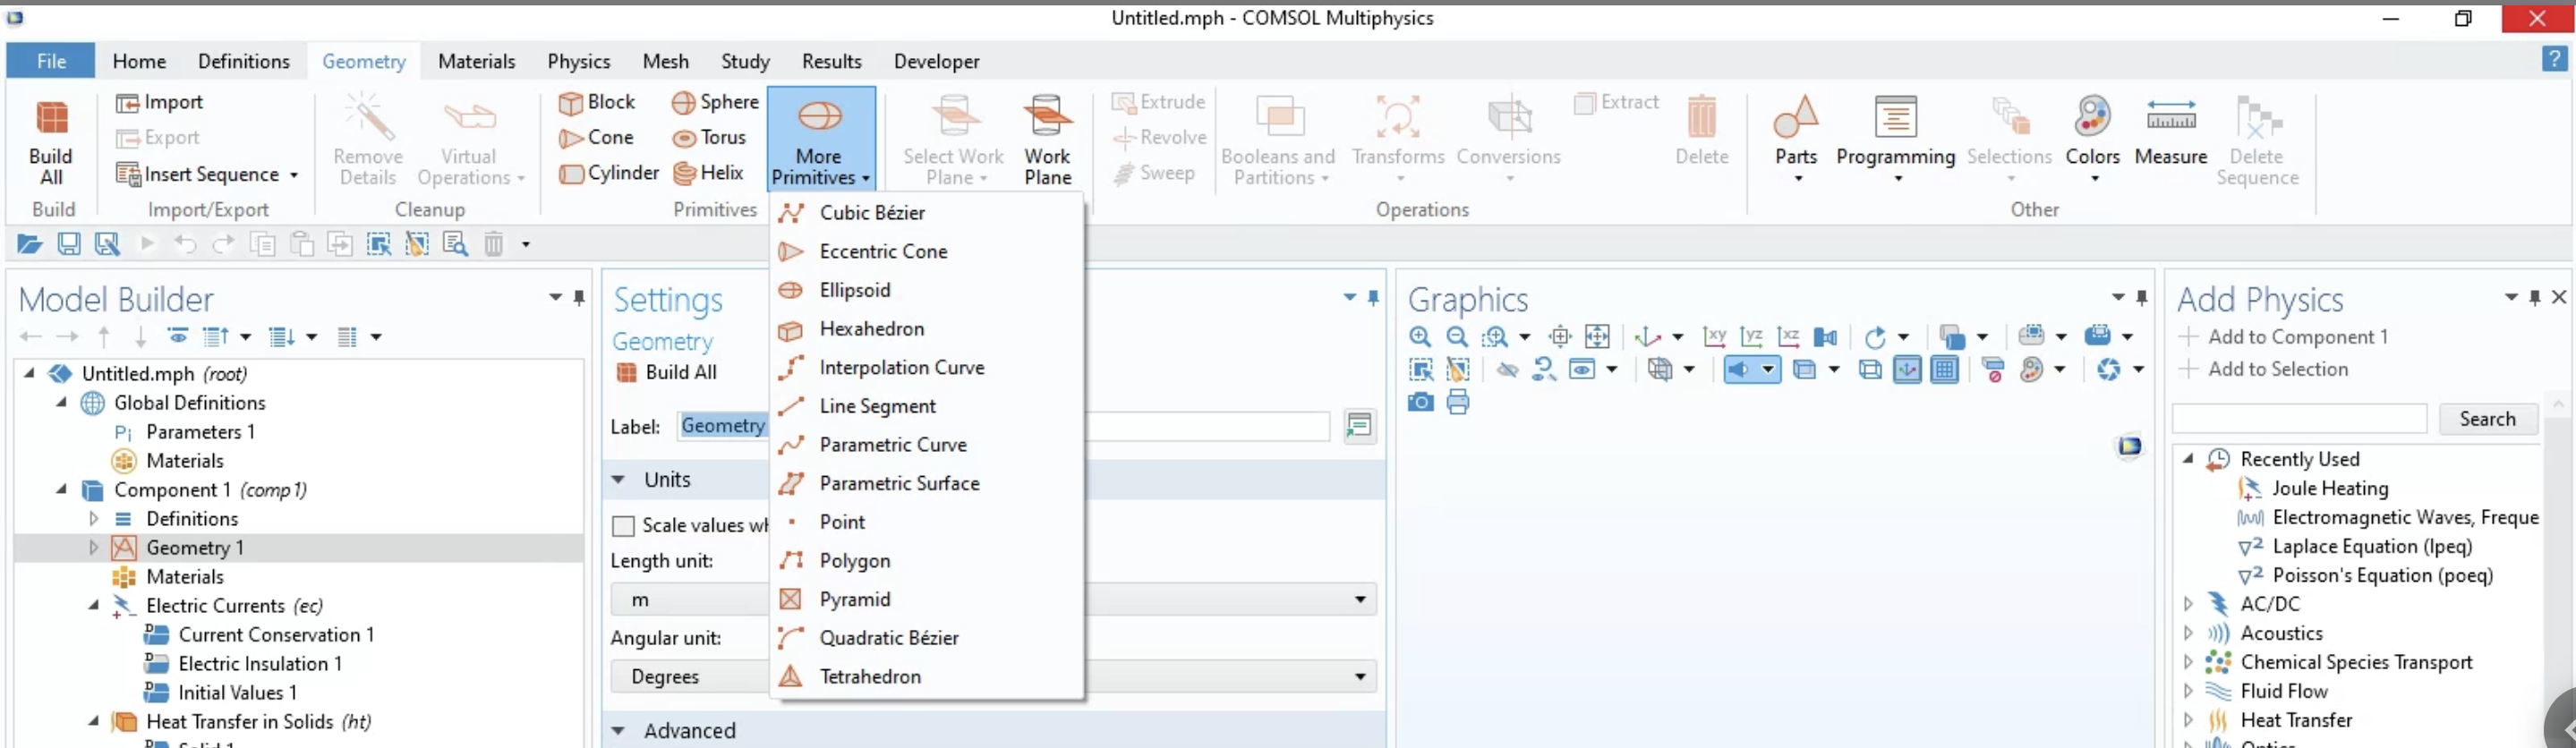
\includegraphics[width=0.4\textwidth]{Chapters/Figures/Chapter 3 Figures/Geometry Tab.png}
  \caption{ Source: \cite{}}
  \label{}
\end{figure}

For this instance, given that the busbar geometry already exists within COMSOL's comprehensive library of pre-configured geometries, accessing this resource simplifies the process. This is achieved by navigating to the File menu and selecting Application Libraries.

% TODO: Add image containing "application libraries" selection
\begin{figure}[ht!]
  \centering
  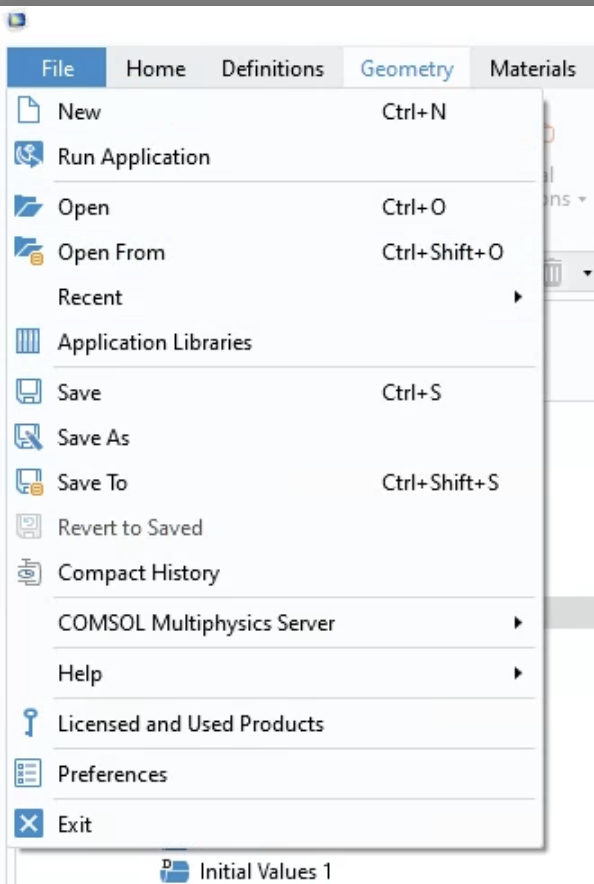
\includegraphics[width=0.4\textwidth]{Chapters/Figures/Chapter 3 Figures/Application Libraries Button.png}
  \caption{ Source: \cite{}}
  \label{}
\end{figure}

Within the Application Libraries, proceed to the COMSOL Multiphysics section, locate the 'busbar\_geom' file, open it, and proceed to save your project accordingly.


% TODO: Add "Application Libraries" image
\begin{figure}[ht!]
  \centering
  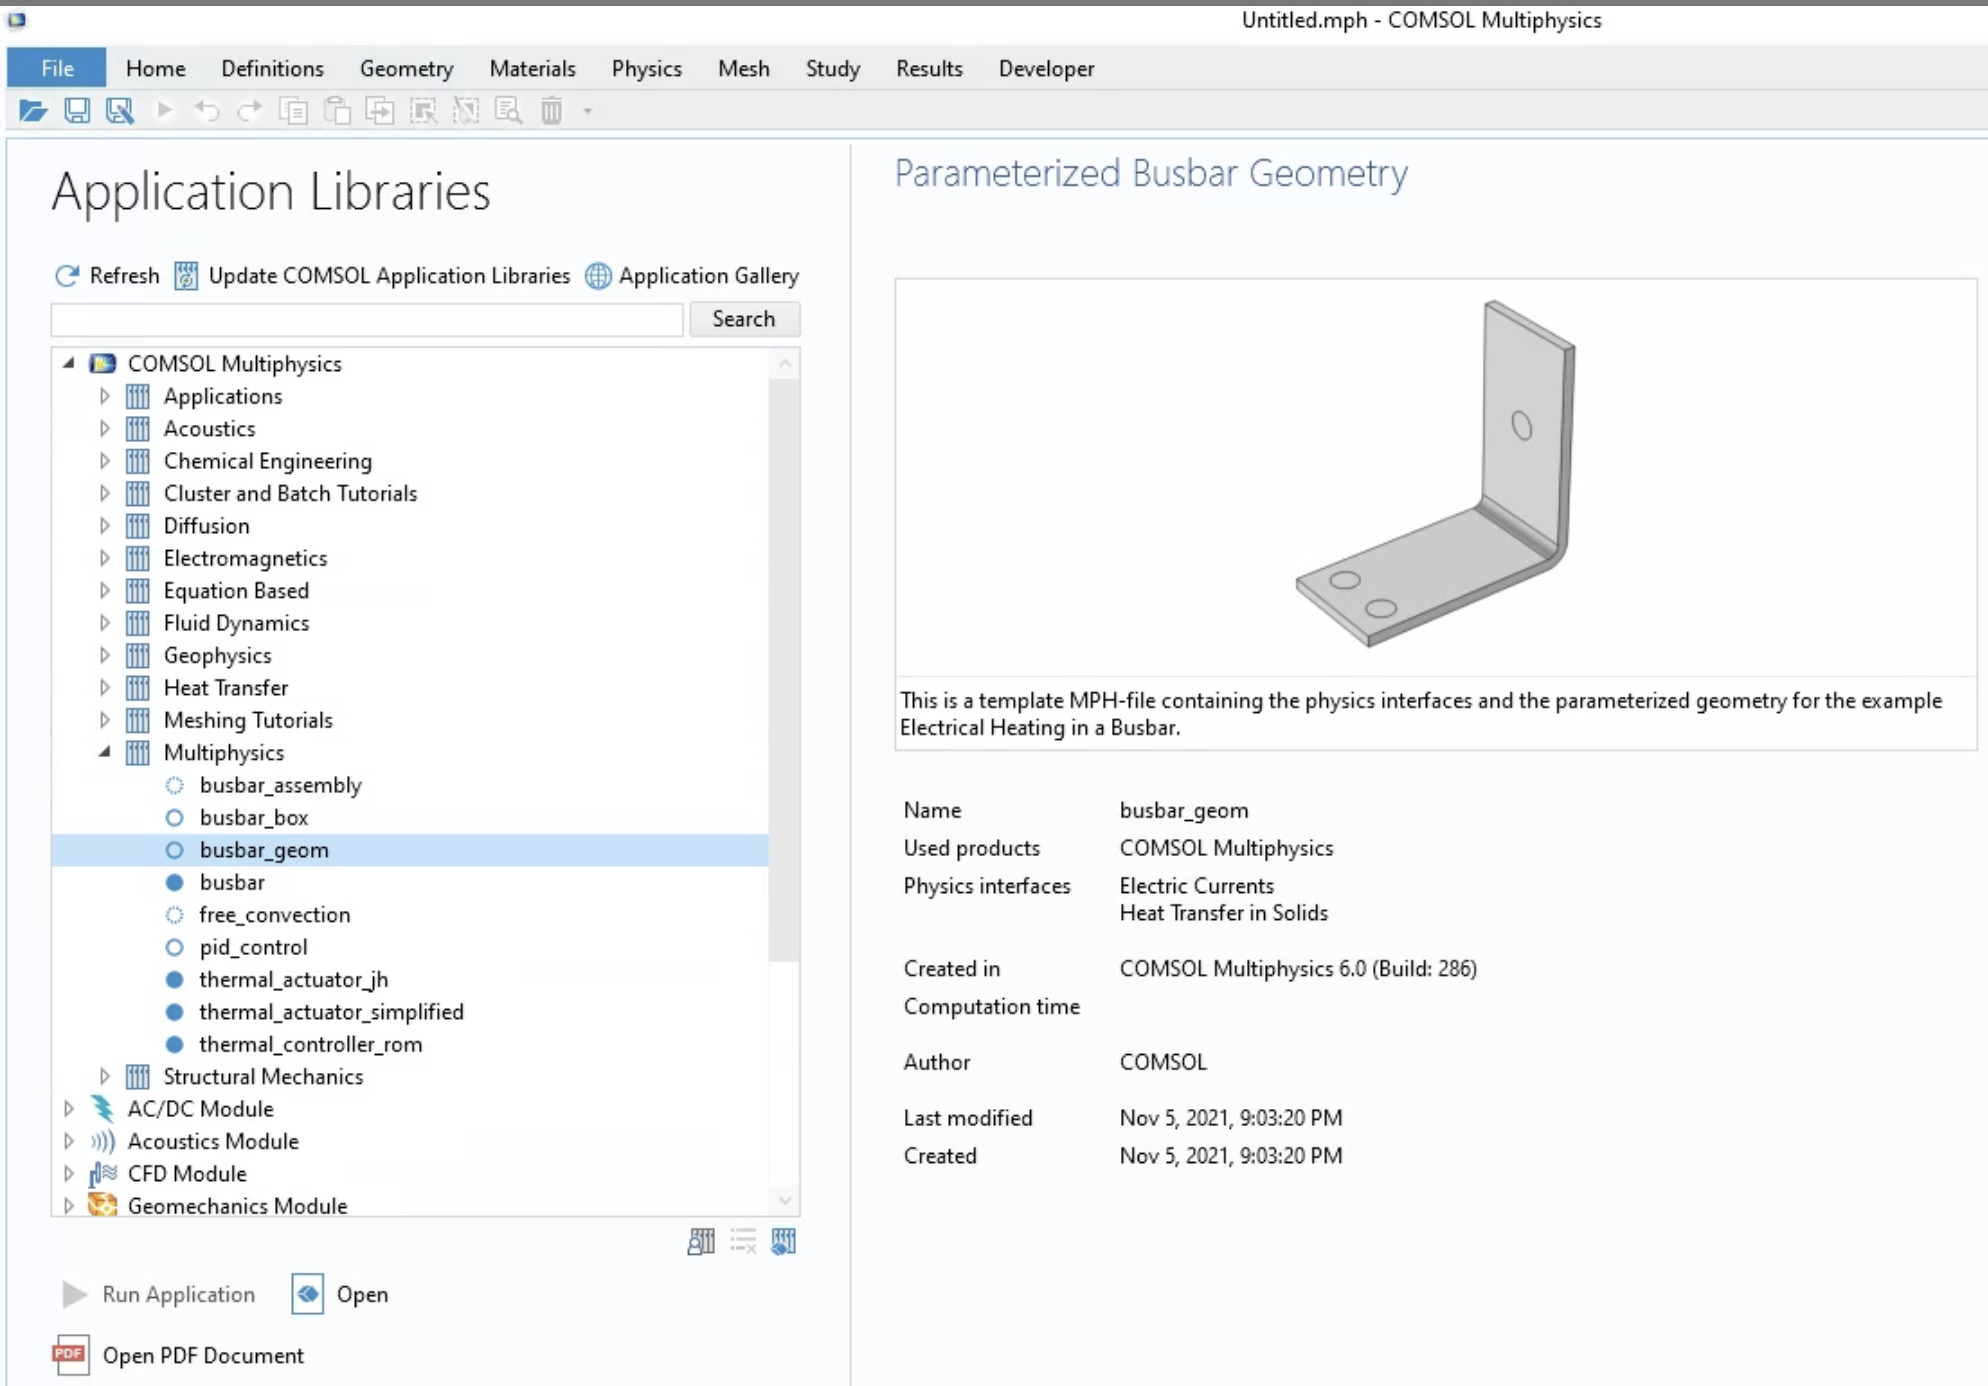
\includegraphics[width=0.4\textwidth]{Chapters/Figures/Chapter 3 Figures/Application Libraries.png}
  \caption{ Source: \cite{}}
  \label{}
\end{figure}

The geometry will now appear in the Graphics window, allowing for zoom and rotational exploration to closely inspect the model. The alteration in the Geometry node within the Model Builder window reflects the sequence of actions executed to construct the busbar geometry. On closer inspection, it becomes evident that specific parameters were employed in crafting this geometry. These parameters are accessible within the ``Parameters 1'' node, which contains a table detailing the adjustable parameters utilized in the geometry's creation.

% TODO: Add image after when you add default busbar geom to model
\begin{figure}[ht!]
  \centering
  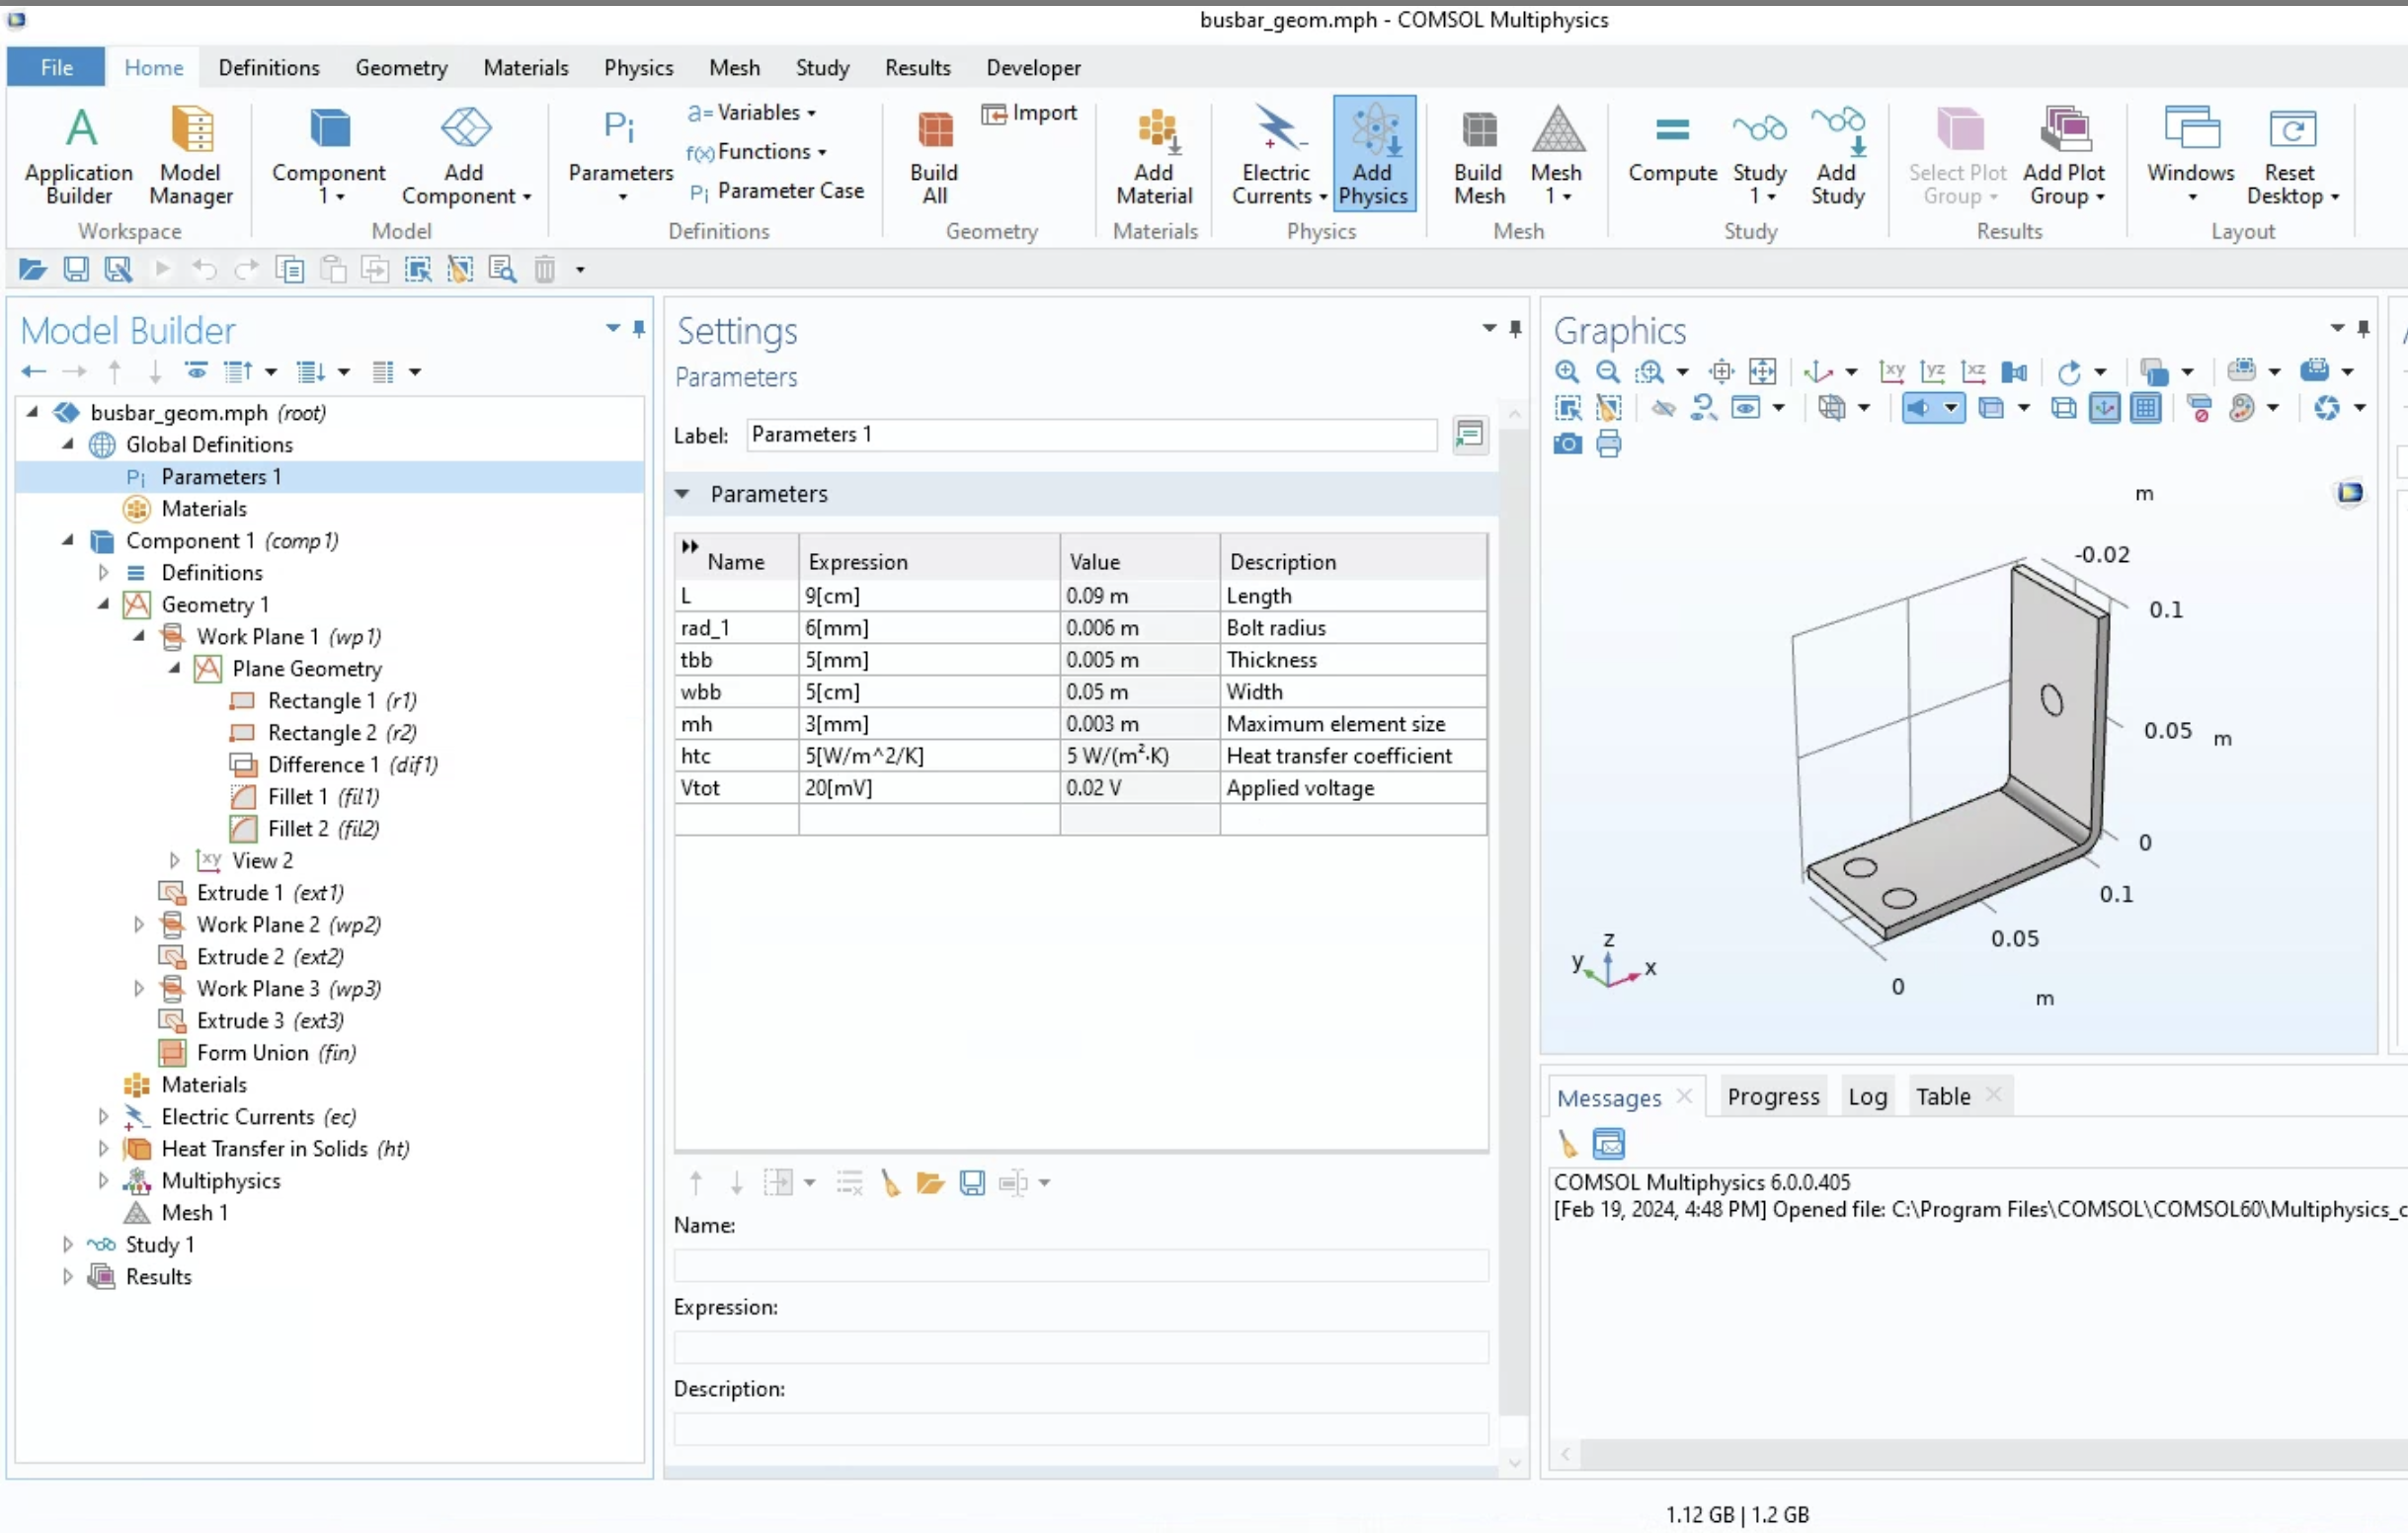
\includegraphics[width=0.4\textwidth]{Chapters/Figures/Chapter 3 Figures/Initial Busbar Geom.png}
  \caption{ Source: \cite{}}
  \label{}
\end{figure}

% SUBSECTION --- Specifying the Material Properties ---
\subsection{Specifying the Material Properties}.

Our busbar comprises various components each requiring distinct materials, necessitating batch assignment of materials to selected parts rather than individual allocation. To commence, access the Definitions tab and opt for the Explicit selection.

% TODO: Add explicit choice selection from Definitions tab
\begin{figure}[ht!]
  \centering
  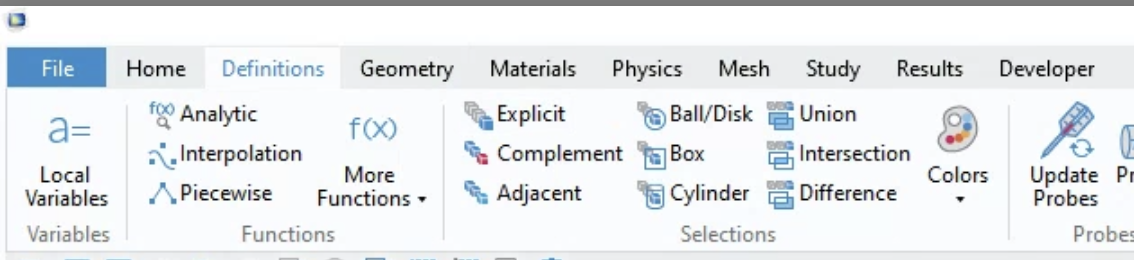
\includegraphics[width=0.4\textwidth]{Chapters/Figures/Chapter 3 Figures/Explicit Choice Selection from Definitions Tab.png}
  \caption{ Source: \cite{}}
  \label{}
\end{figure}

Following this, in the Graphics window, we identify and select the bolts, ensuring both their front and back sides are chosen due to their differing material composition from the busbar's main body.

% TODO: Add bolt selections after selections
\begin{figure}[ht!]
  \centering
  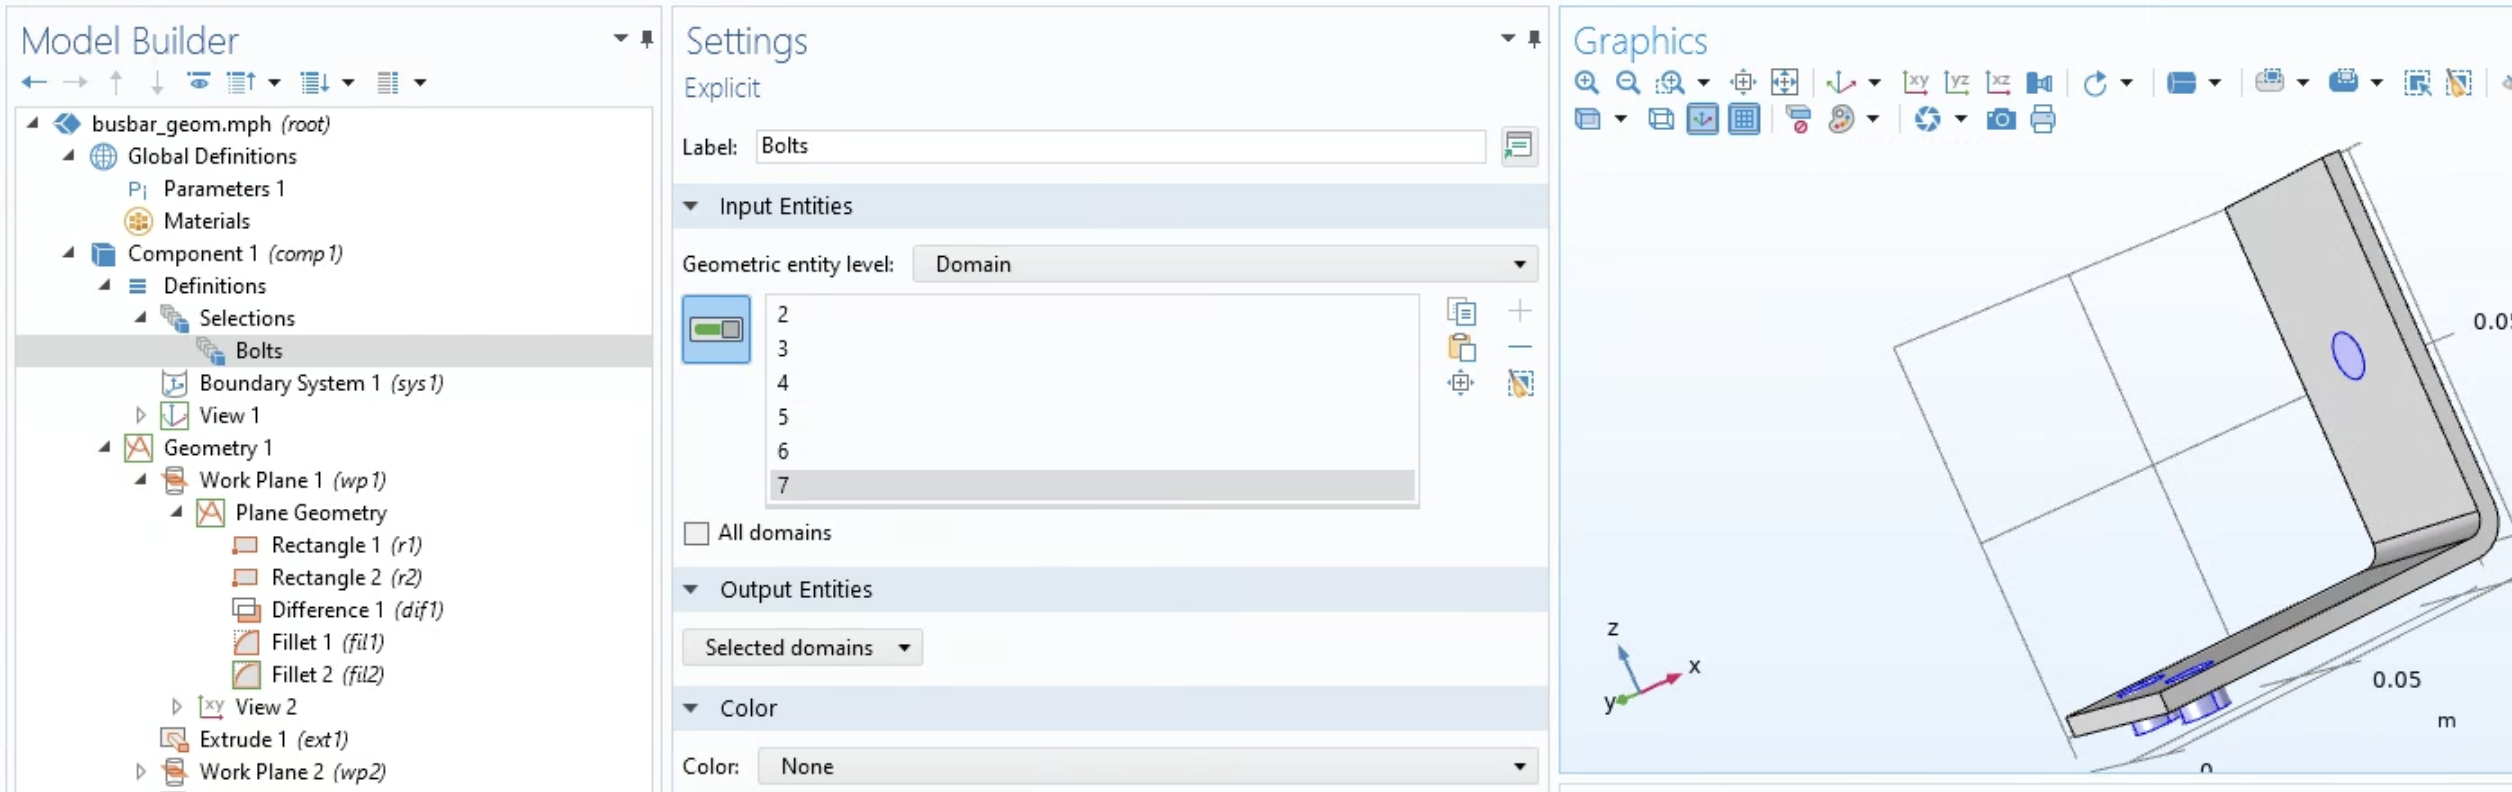
\includegraphics[width=0.4\textwidth]{Chapters/Figures/Chapter 3 Figures/Bolts Selection.png}
  \caption{ Source: \cite{}}
  \label{}
\end{figure}

Proceeding to material assignment, we move to the Materials ribbon and select the Add Materials feature. This action opens the ``Add Material'' window, offering a selection of materials to apply to the chosen components.

% TODO: Add the Add Materials image
\begin{figure}[ht!]
  \centering
  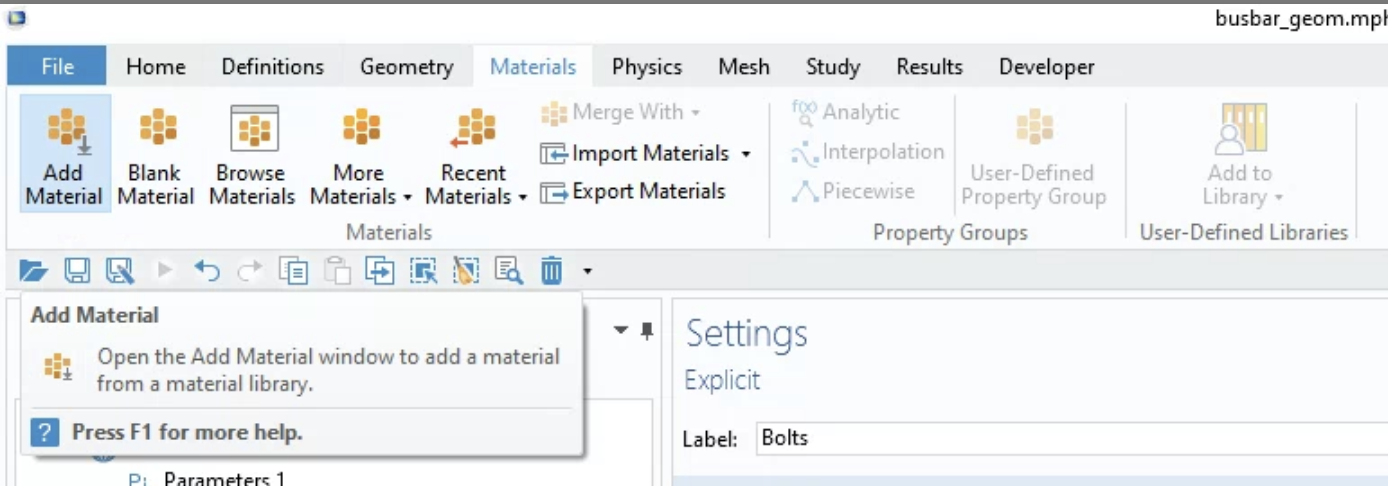
\includegraphics[width=0.4\textwidth]{Chapters/Figures/Chapter 3 Figures/Add Material Button.png}
  \caption{Source: \cite{}}
  \label{}
\end{figure}

Select the Built-In option and opt for Titanium (for the bolts) and Copper as the materials.

% TODO: Add the Add Materials window image
\begin{figure}[ht!]
  \centering
  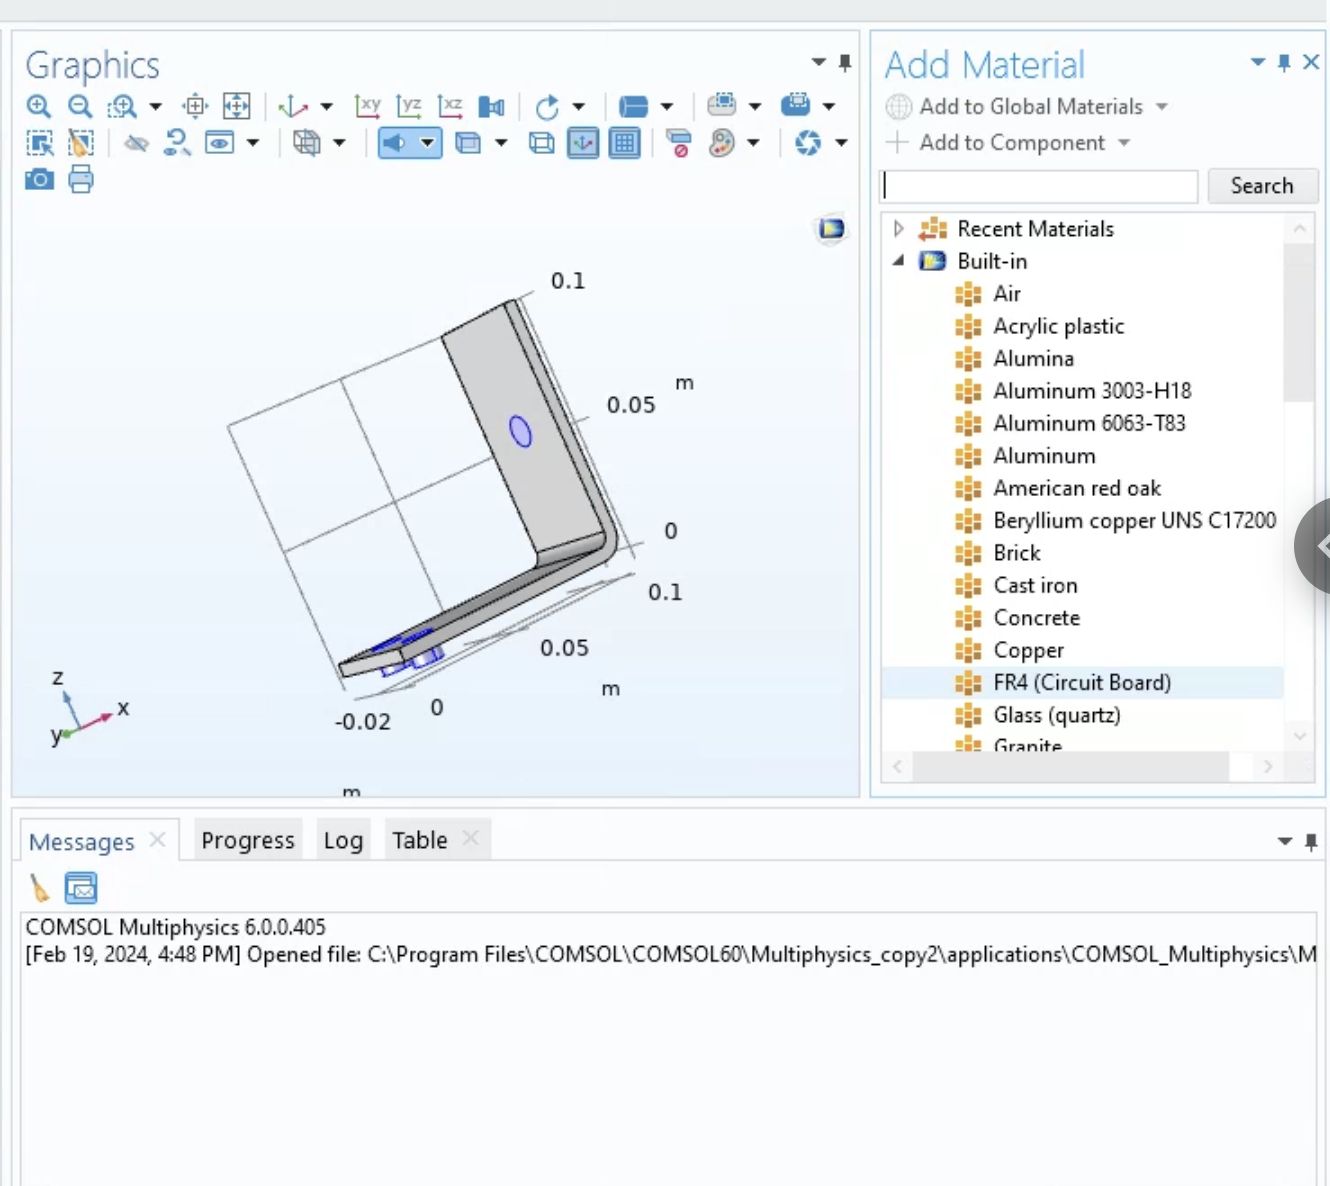
\includegraphics[width=0.4\textwidth]{Chapters/Figures/Chapter 3 Figures/Add Material Window.png}
  \caption{Source: \cite{}}
  \label{}
\end{figure}

The earlier defined selection for Bolts proves useful now as we assign Titanium to each bolt by selecting the Bolts option, as illustrated below.

% TODO: Add the bolts for titanium material selection
\begin{figure}[ht!]
  \centering
  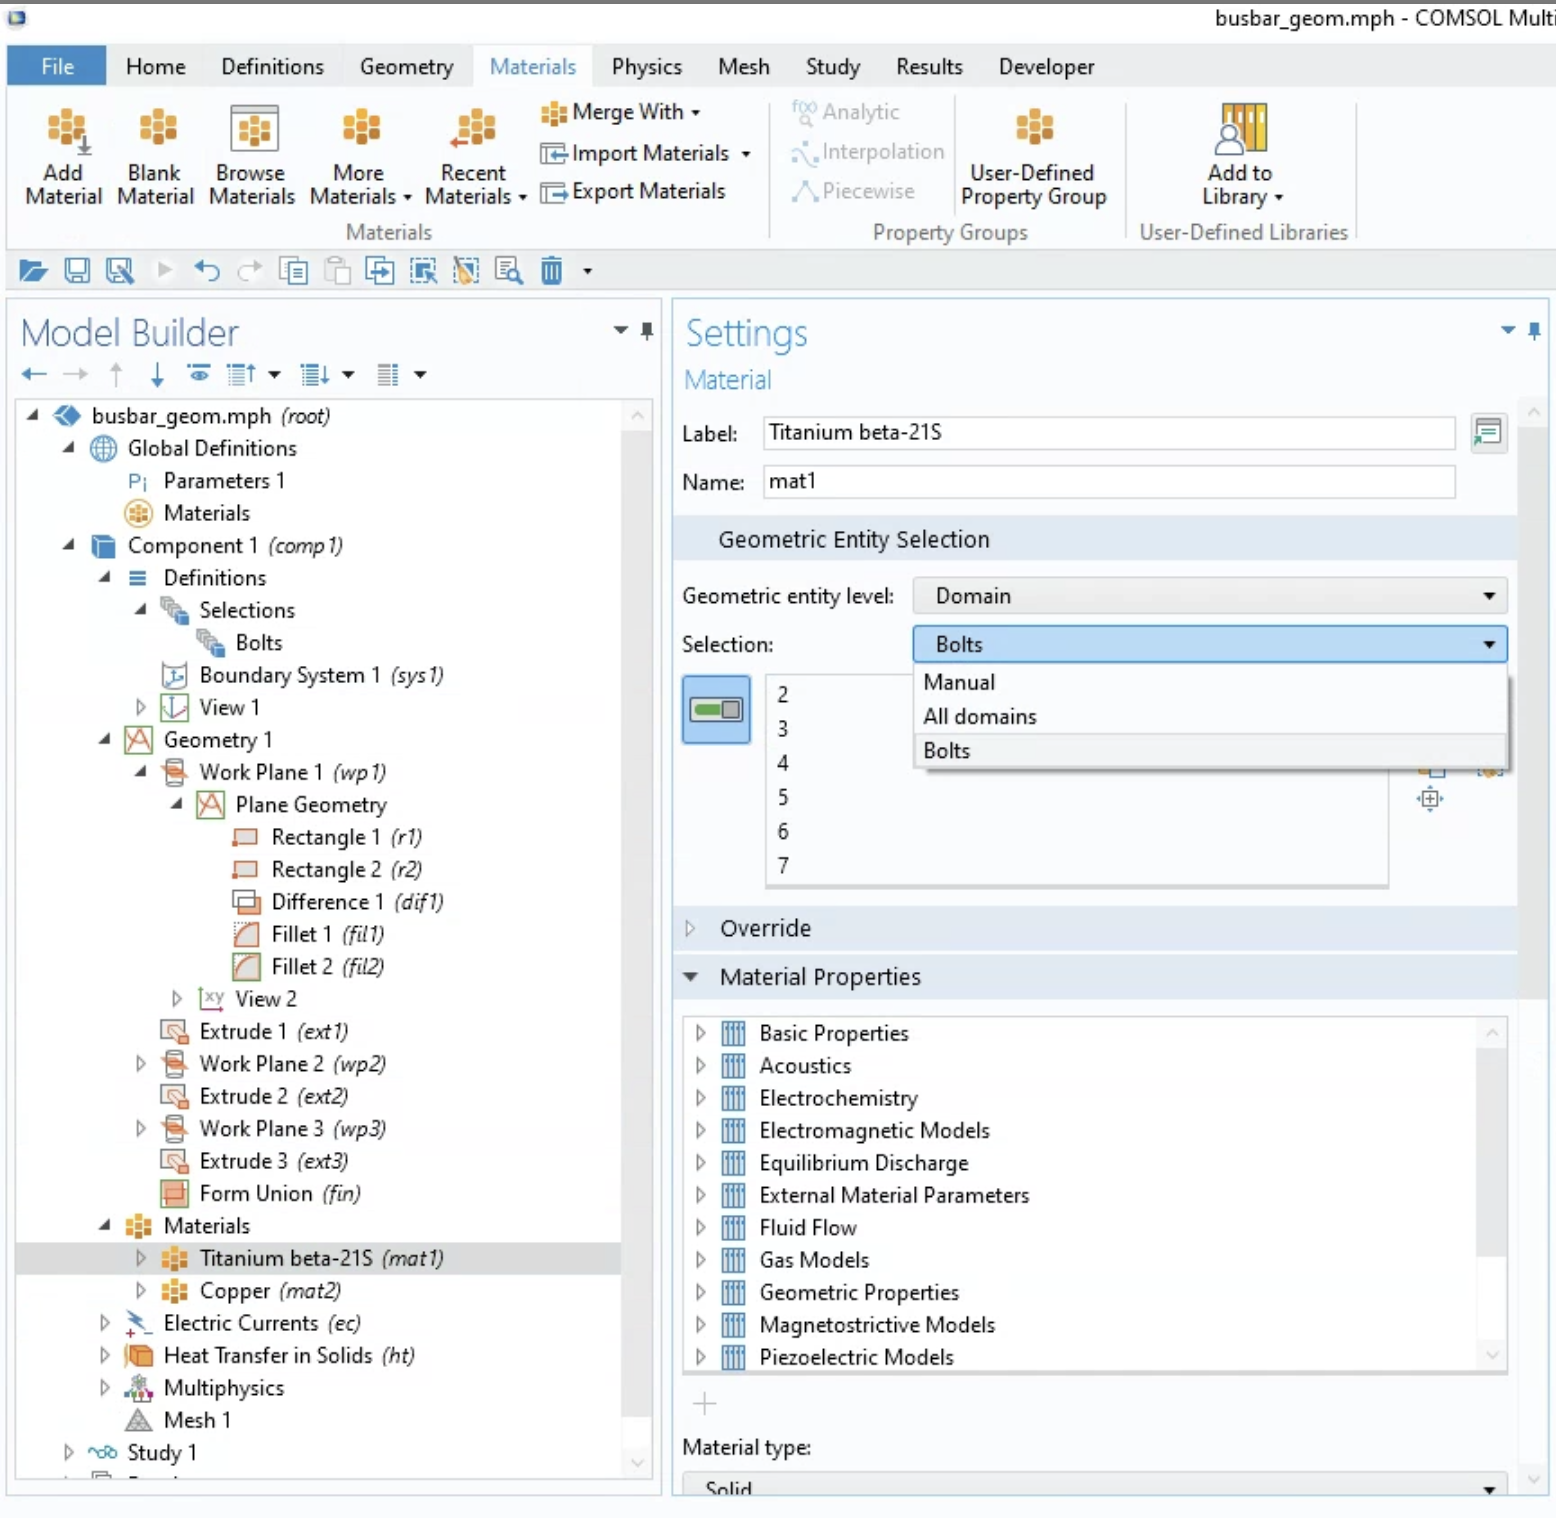
\includegraphics[width=0.4\textwidth]{Chapters/Figures/Chapter 3 Figures/Bolts Selection Choice.png}
  \caption{Source: \cite{}}
  \label{}
\end{figure}

Every time a material is added, and consequently, a material node is introduced in the Model Builder window, a table appears in the Settings window under Material Contents. This table details the physical properties of the respective materials, including Electrical Conductivity, Heat Capacity, and more.

% TODO: Add image showing material contents (properties)
\begin{figure}[ht!]
  \centering
  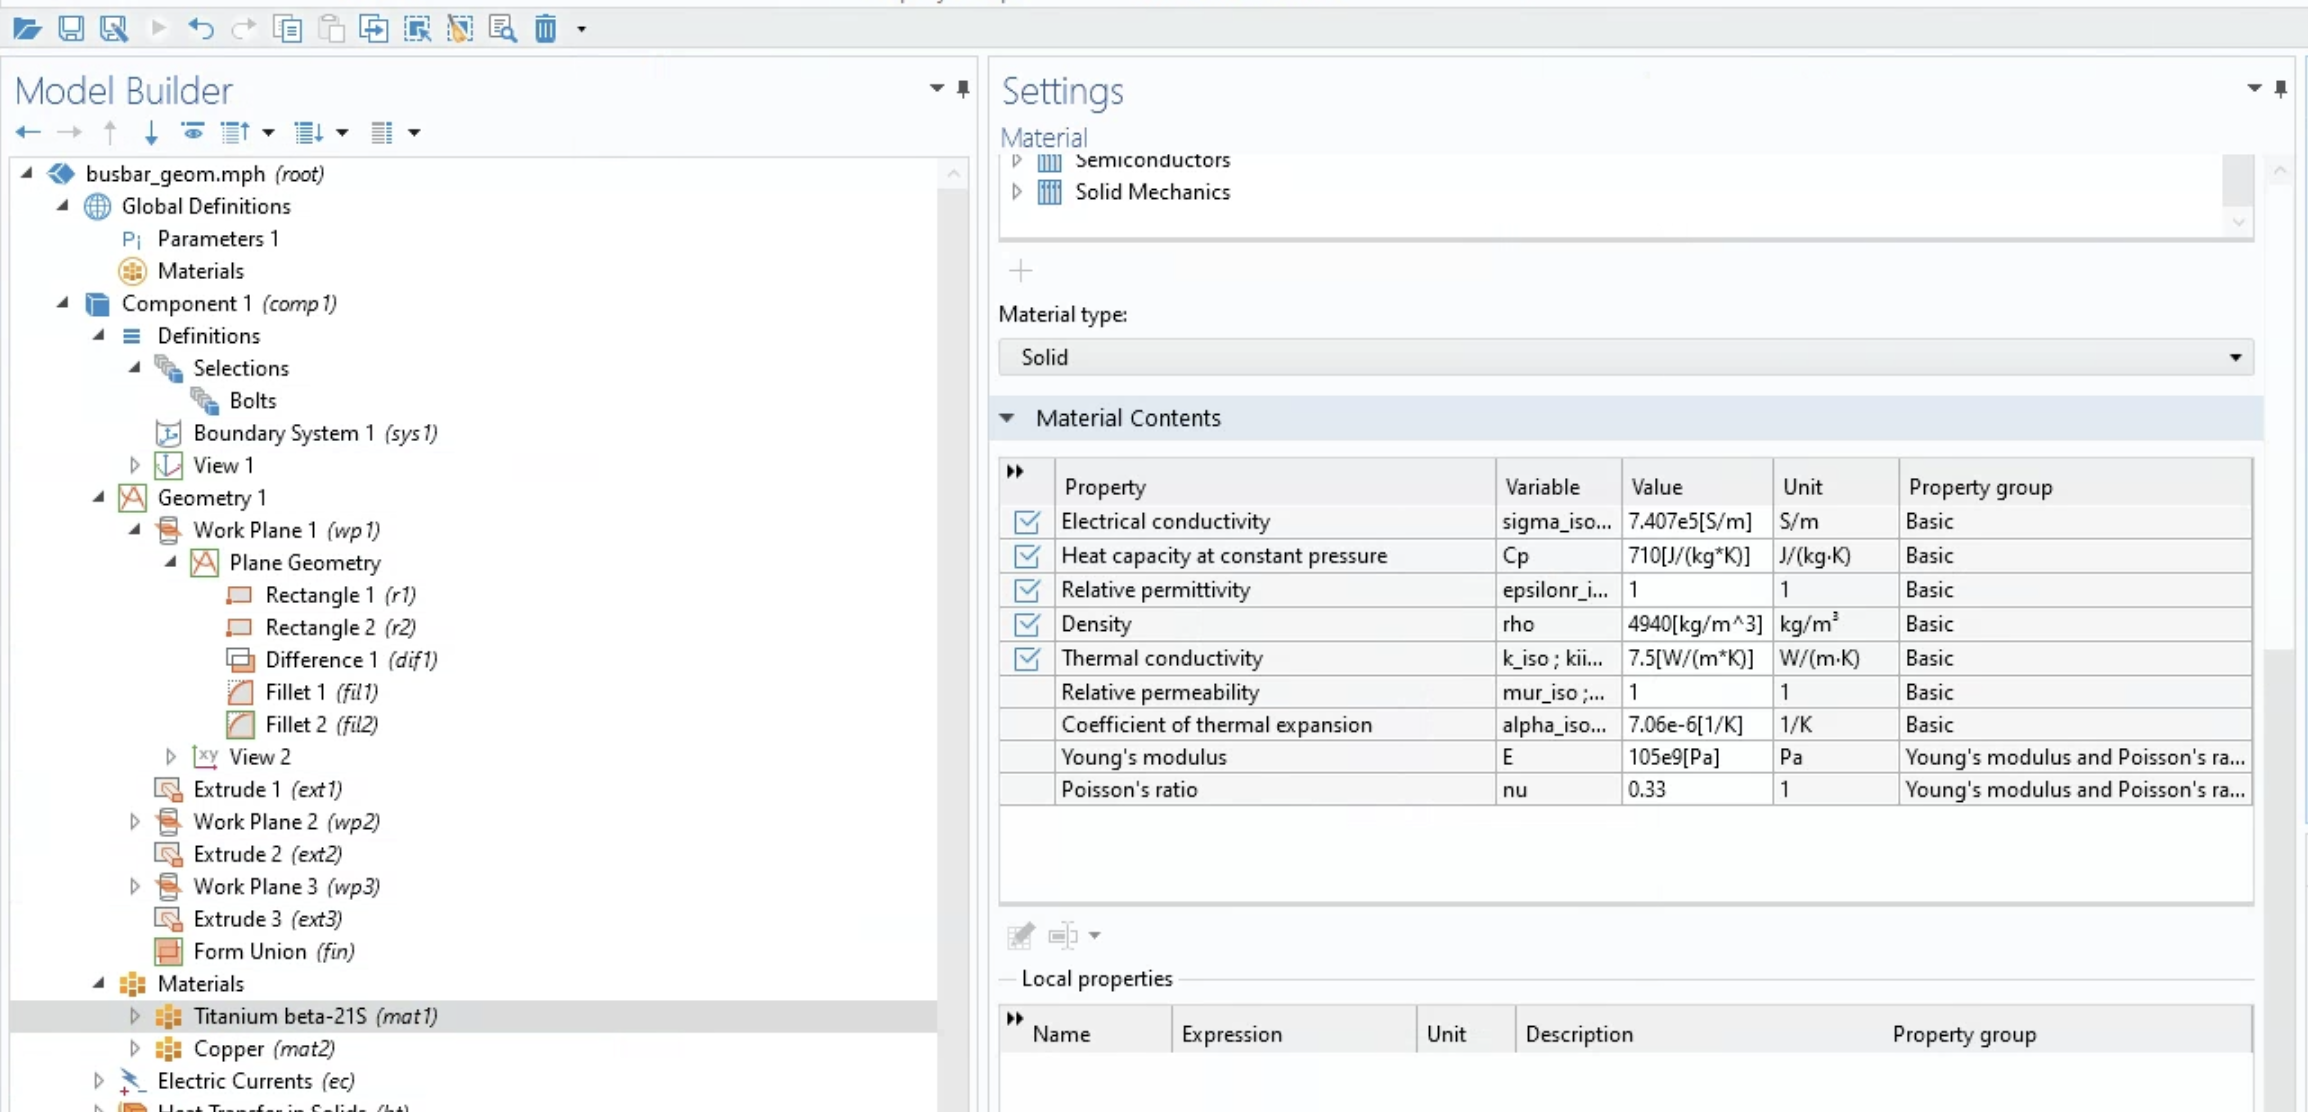
\includegraphics[width=0.4\textwidth]{Chapters/Figures/Chapter 3 Figures/Material Contents in Settings Window.png}
  \caption{Source: \cite{}}
  \label{}
\end{figure}


% SUBSECTION --- Defining the Physics Boundary Conditions ---
\subsection{Defining the Physics Boundary Conditions}.
It's time to apply mathematical formulas across various sections of our model to replicate the intended physics. This involves highlighting specific segments of the geometry and imposing relevant formulas and physical parameters that accurately represent those segments.

We'll begin by setting up the physics for the electric current interface, aiming to model the flow of electricity from a singular bolt across to the twin bolts at the opposite end of the busbar. The specific physics chosen during the initial model setup might already have certain equations predefined within their physics nodes. For example, within the ``Electric Currents (ec)'' node, the settings window reveals equations pertinent to this physics. A key equation presented is the fundamental one linking the electric field with electric potential, expressed as $\mathbf{E} = -\nabla V$.

% TODO: Add image showing equation
\begin{figure}[ht!]
  \centering
  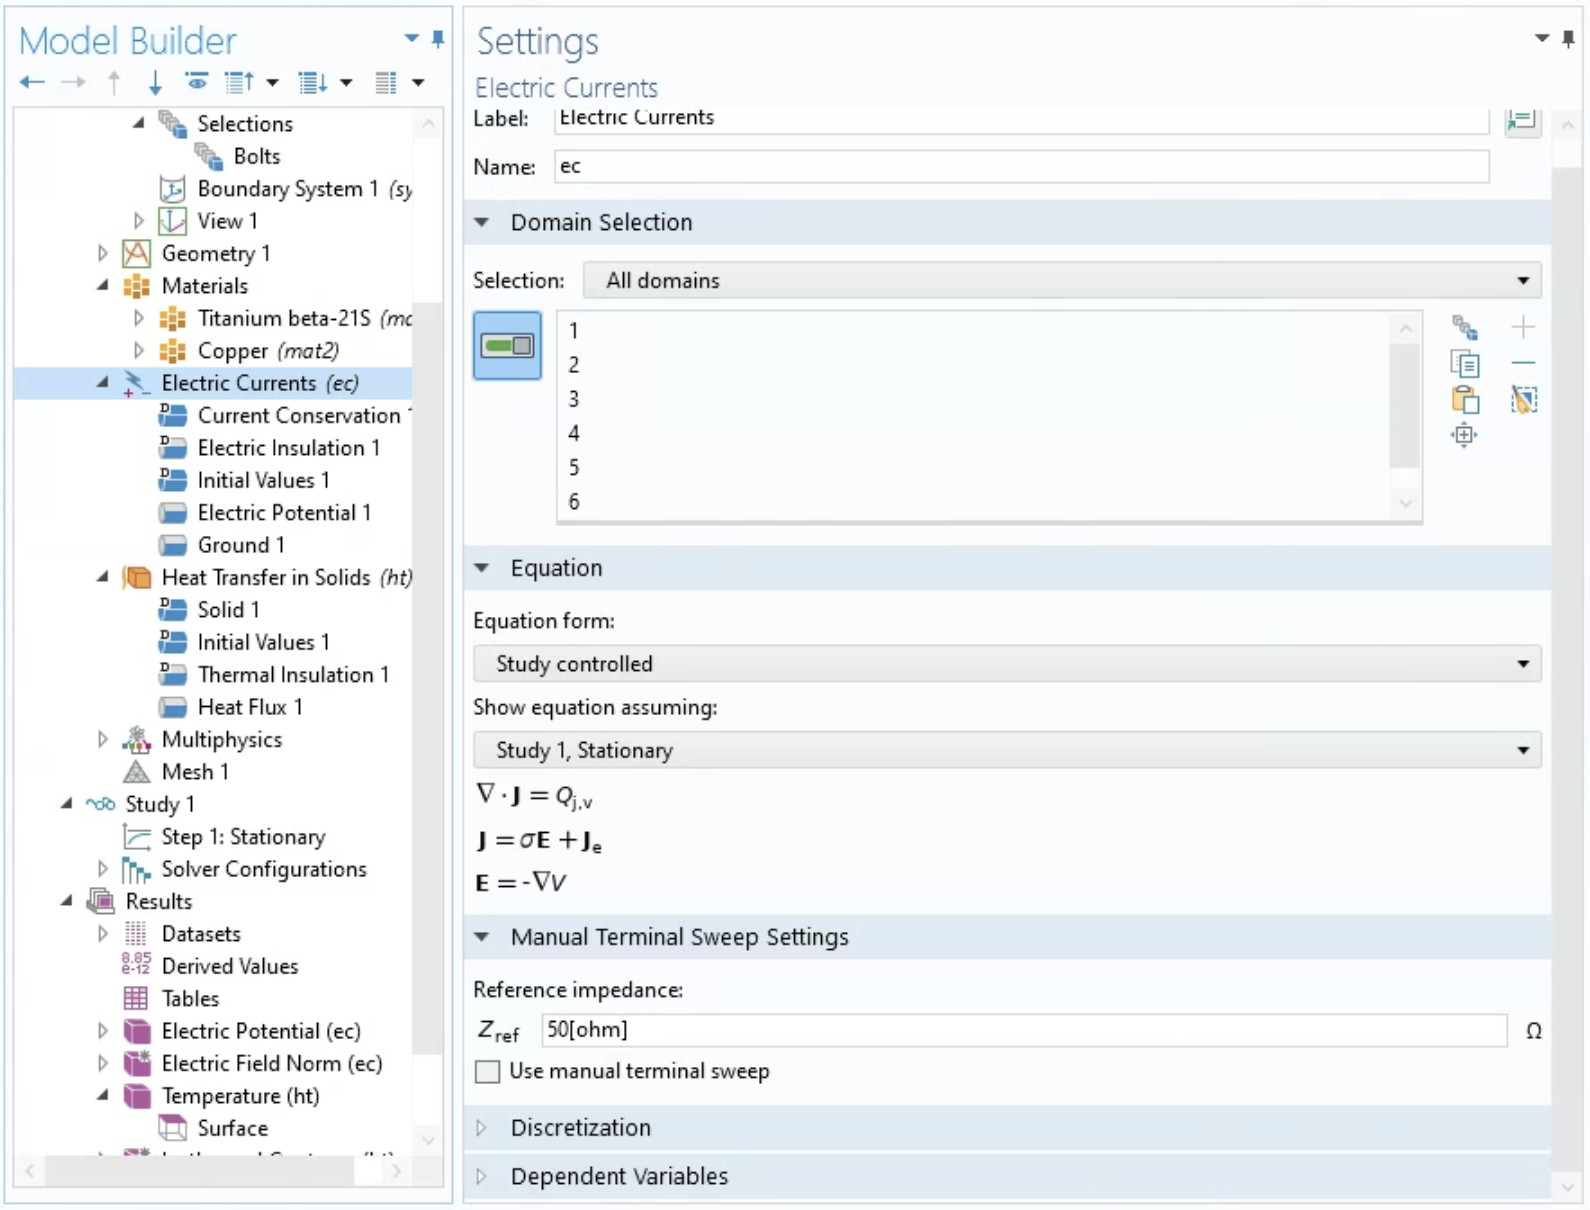
\includegraphics[width=0.4\textwidth]{Chapters/Figures/Chapter 3 Figures/Electrical Currents Physics Equation.png}
  \caption{Source: \cite{}}
  \label{}
\end{figure}

COMSOL Multiphysics operates transparently, allowing users to fully grasp the software's actions and methodologies.

Upon integrating physics into our model, several default nodes were automatically established within each physics category. We add specific boundary conditions and constraints only if they deviate from these defaults. For example, the ``Electric Currents (ec)'' physics automatically applies the ``Electric Insulation 1'' condition to all boundaries, which may not suit our model's requirements.

For our purpose, we aim to impose a voltage on the bottom surface of the single bolt. This is achieved by navigating to the Physics tab, selecting Boundaries, and then choosing Electric Potential. This action adds an ``Electric Potential 1'' node. The next step is to identify and select the geometry segment this potential will affect. To specify the electric potential value, we input 20 mV, denoted as 20[mV], with the brackets indicating unit specification.

To simplify the process, remember that the ``Parameters 1'' node contains a predefined variable, Vtot, representing the applied voltage. Utilizing this variable instead of inputting 20[mV] directly facilitates the setup of parametric studies in the future.

Finally, to complete our setup, we establish a ground boundary condition on the bottom surfaces of the two bolts at the busbar's opposite end. This is accomplished by selecting Ground from the Physics tab's boundaries options, then choosing the relevant geometry segments.

% TODO: Add image showing "Electric Currents" boundary conditions
\begin{figure}[ht!]
  \centering
  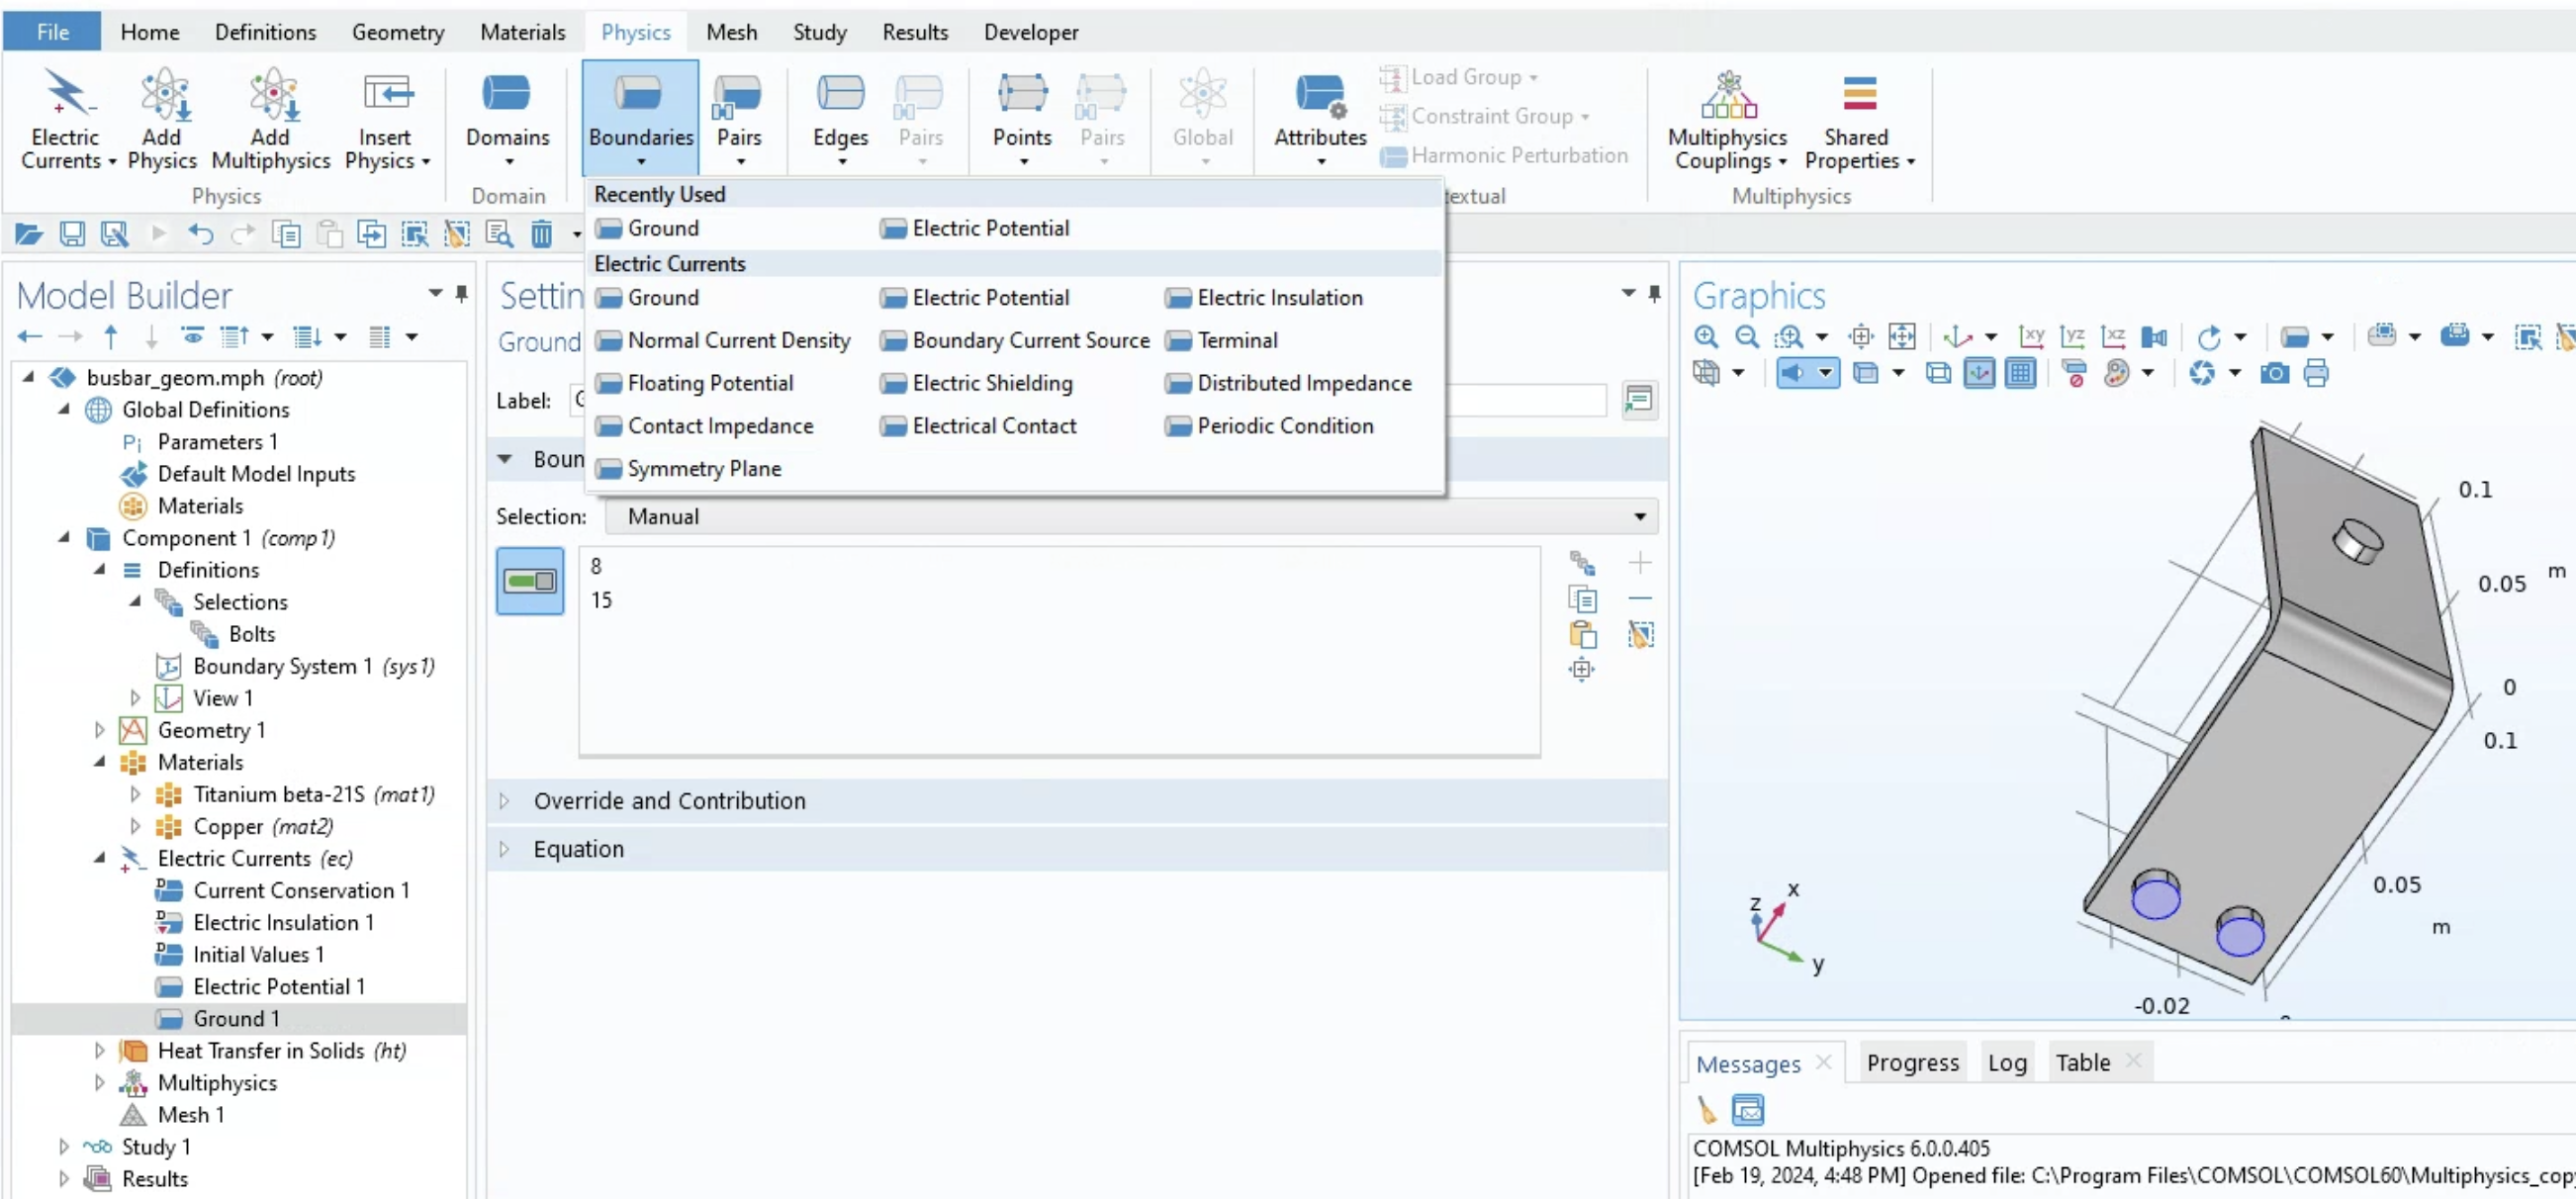
\includegraphics[width=0.4\textwidth]{Chapters/Figures/Chapter 3 Figures/Electric Currents Boundary Conditions.png}
  \caption{Source: \cite{}}
  \label{}
\end{figure}

Given the selection of Joule Heating as a coupled physics in our model, it's essential to define the thermal boundary conditions as well. The default ``Thermal Insulation 1'' condition, which applies universally across our model, does not suit our specific needs. To address this, proceed to the Physics tab, access Boundaries, and opt for Heat Flux. Within the settings, under Boundary Selection, choose ``All Boundaries'' but exclude the previously selected bolt surfaces for the Electric Currents boundaries—namely, boundaries 8, 15, and 43—by deselecting these numbers using the ``Remove from Selection'' option.

For the Heat Flux settings, opt for the ``Convective heat flux'' under the Flux Type category, entering a value of 5 $W/(m^2\cdot K)$. Similar to our approach with the electric potential, revert to the Parameters 1 node and input htc, which denotes the value of 5 $W/(m^2\cdot K)$.

% TODO: Add image showing Heat Flux boundary conditions
\begin{figure}[ht!]
  \centering
  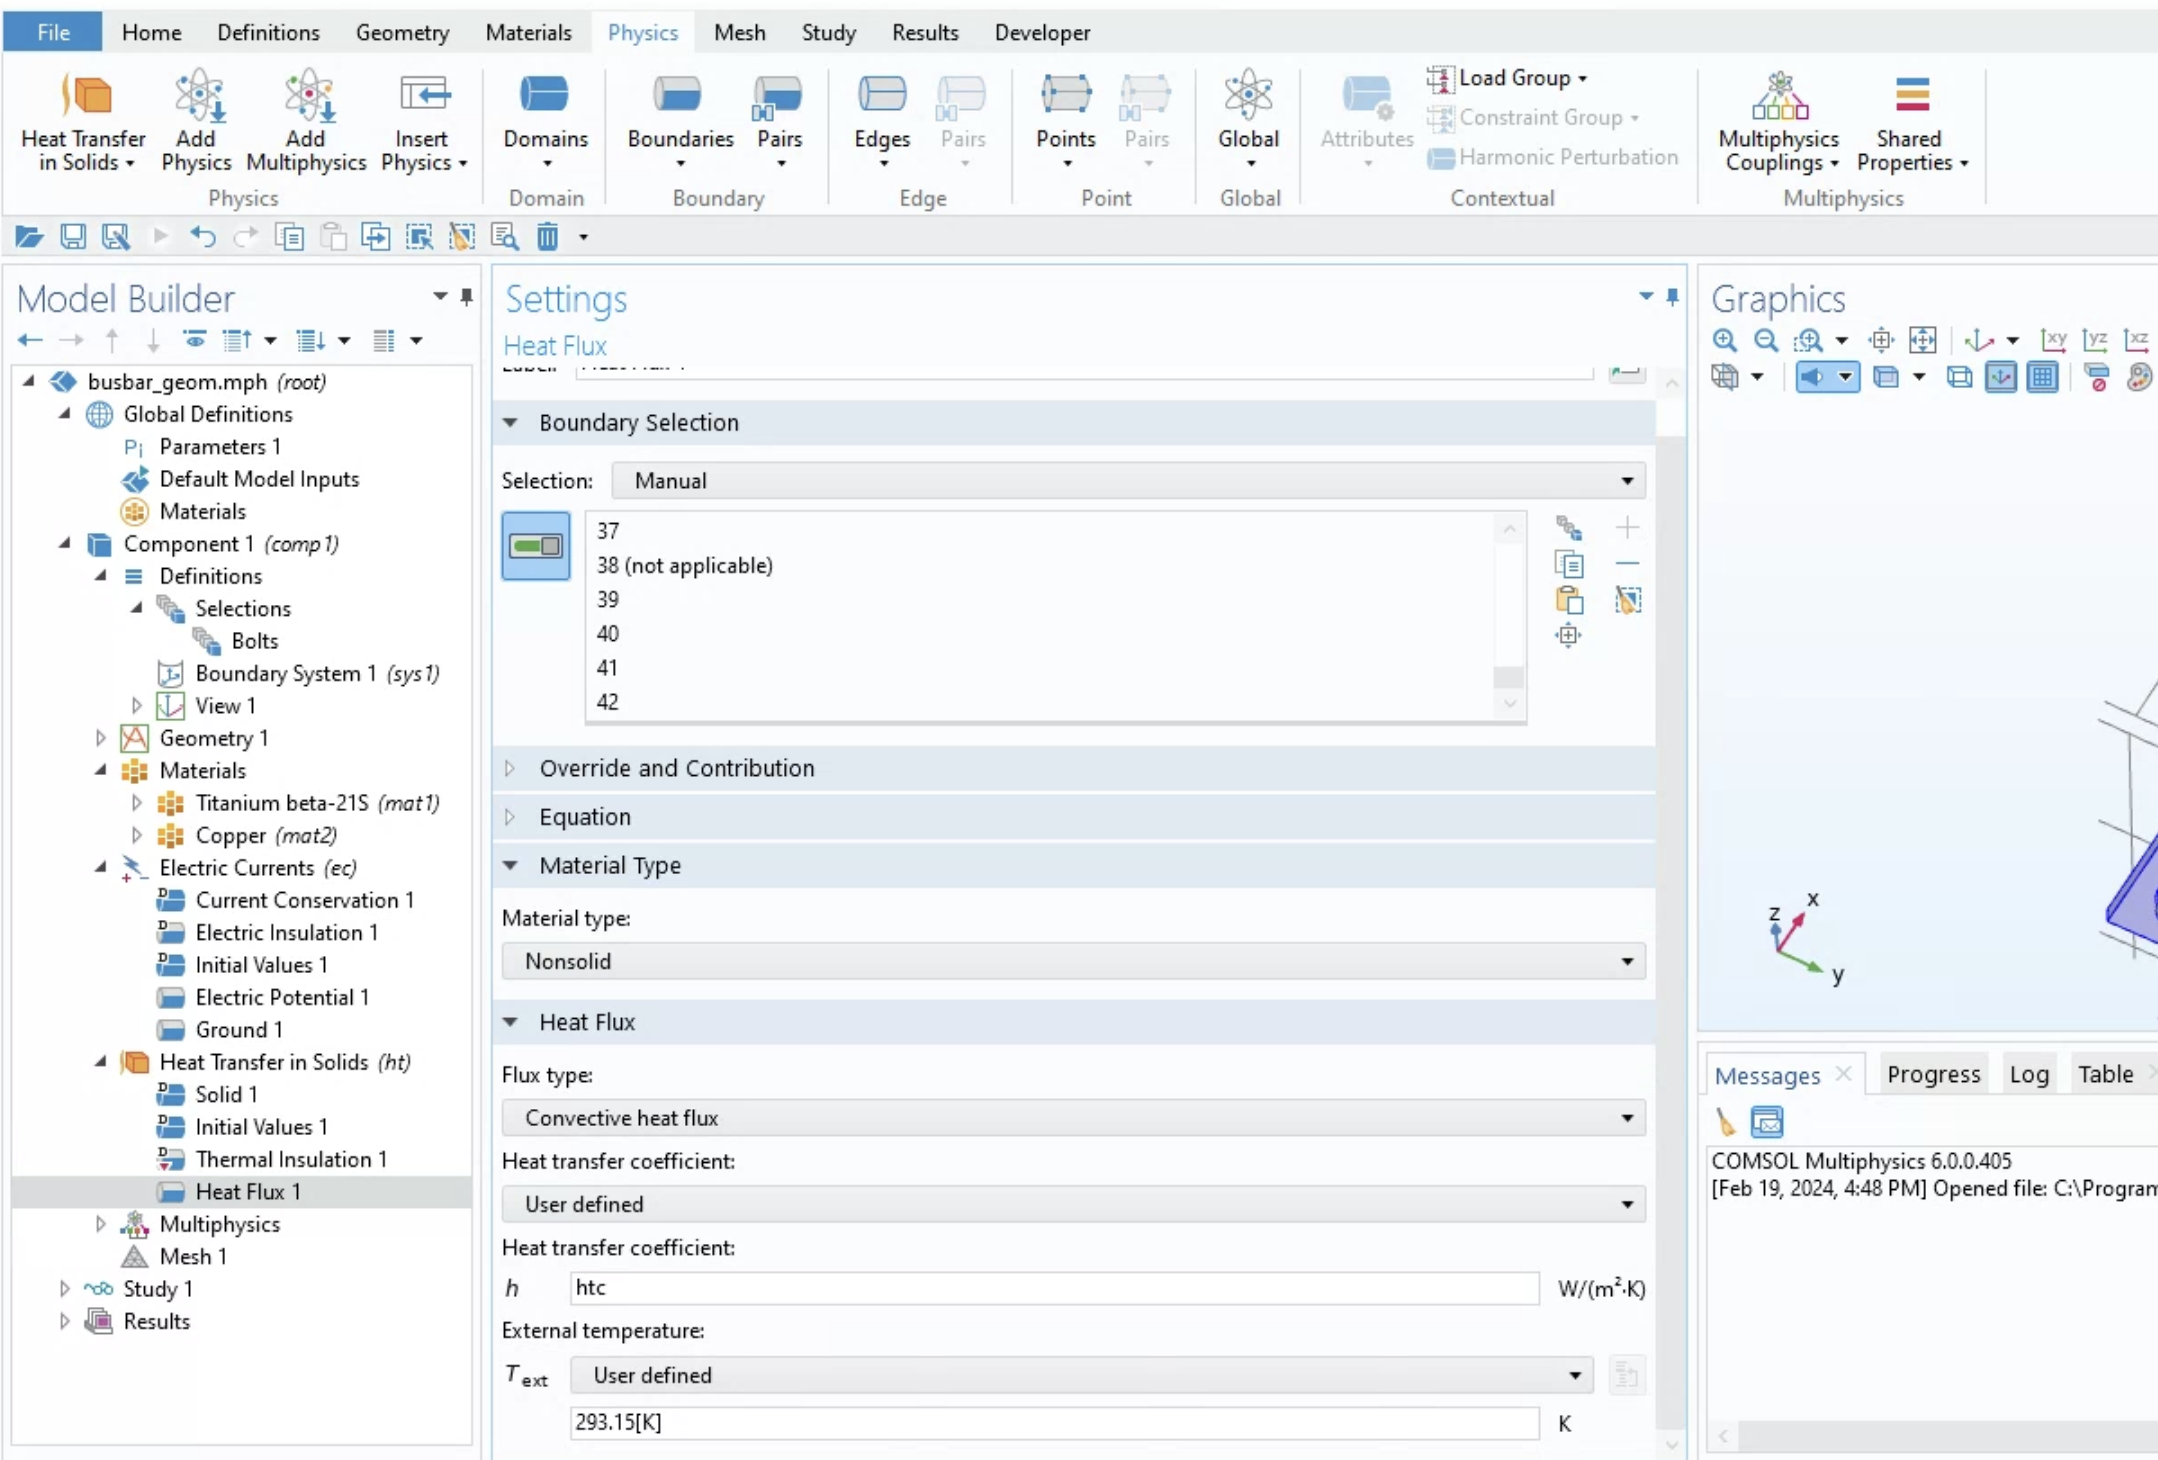
\includegraphics[width=0.4\textwidth]{Chapters/Figures/Chapter 3 Figures/Heat Flux Boundary Conditions.png}
  \caption{Source: \cite{}}
  \label{}
\end{figure}

In our busbar model, the two physics components we've incorporated, namely Electric Currents and Heat Transfer in solids, are universally applicable throughout the model.

% SUBSECTION --- Build the Mesh ---
\subsection{Build the Mesh}.
Navigate to the Mesh ribbon and initiate mesh configuration by selecting ``Mesh 1.'' Within the Settings, under Mesh Setting, accessing the Sequence Type menu presents two alternatives: the default Physics-controlled mesh, which automatically tailors the mesh to the model's physics requirements, and the user-controlled mesh, granting manual oversight over mesh granularity and enabling the use of diverse element types.

COMSOL Multiphysics accommodates a variety of 2D and 3D element shapes, including pyramids, triangles, and prisms. The software offers nine predefined element size settings, ranging from extremely fine to extremely coarse. To construct the mesh, simply press the ``Build All'' button.

% TODO: Add image showing the mesh of the busbar under "fine"
\begin{figure}[ht!]
  \centering
  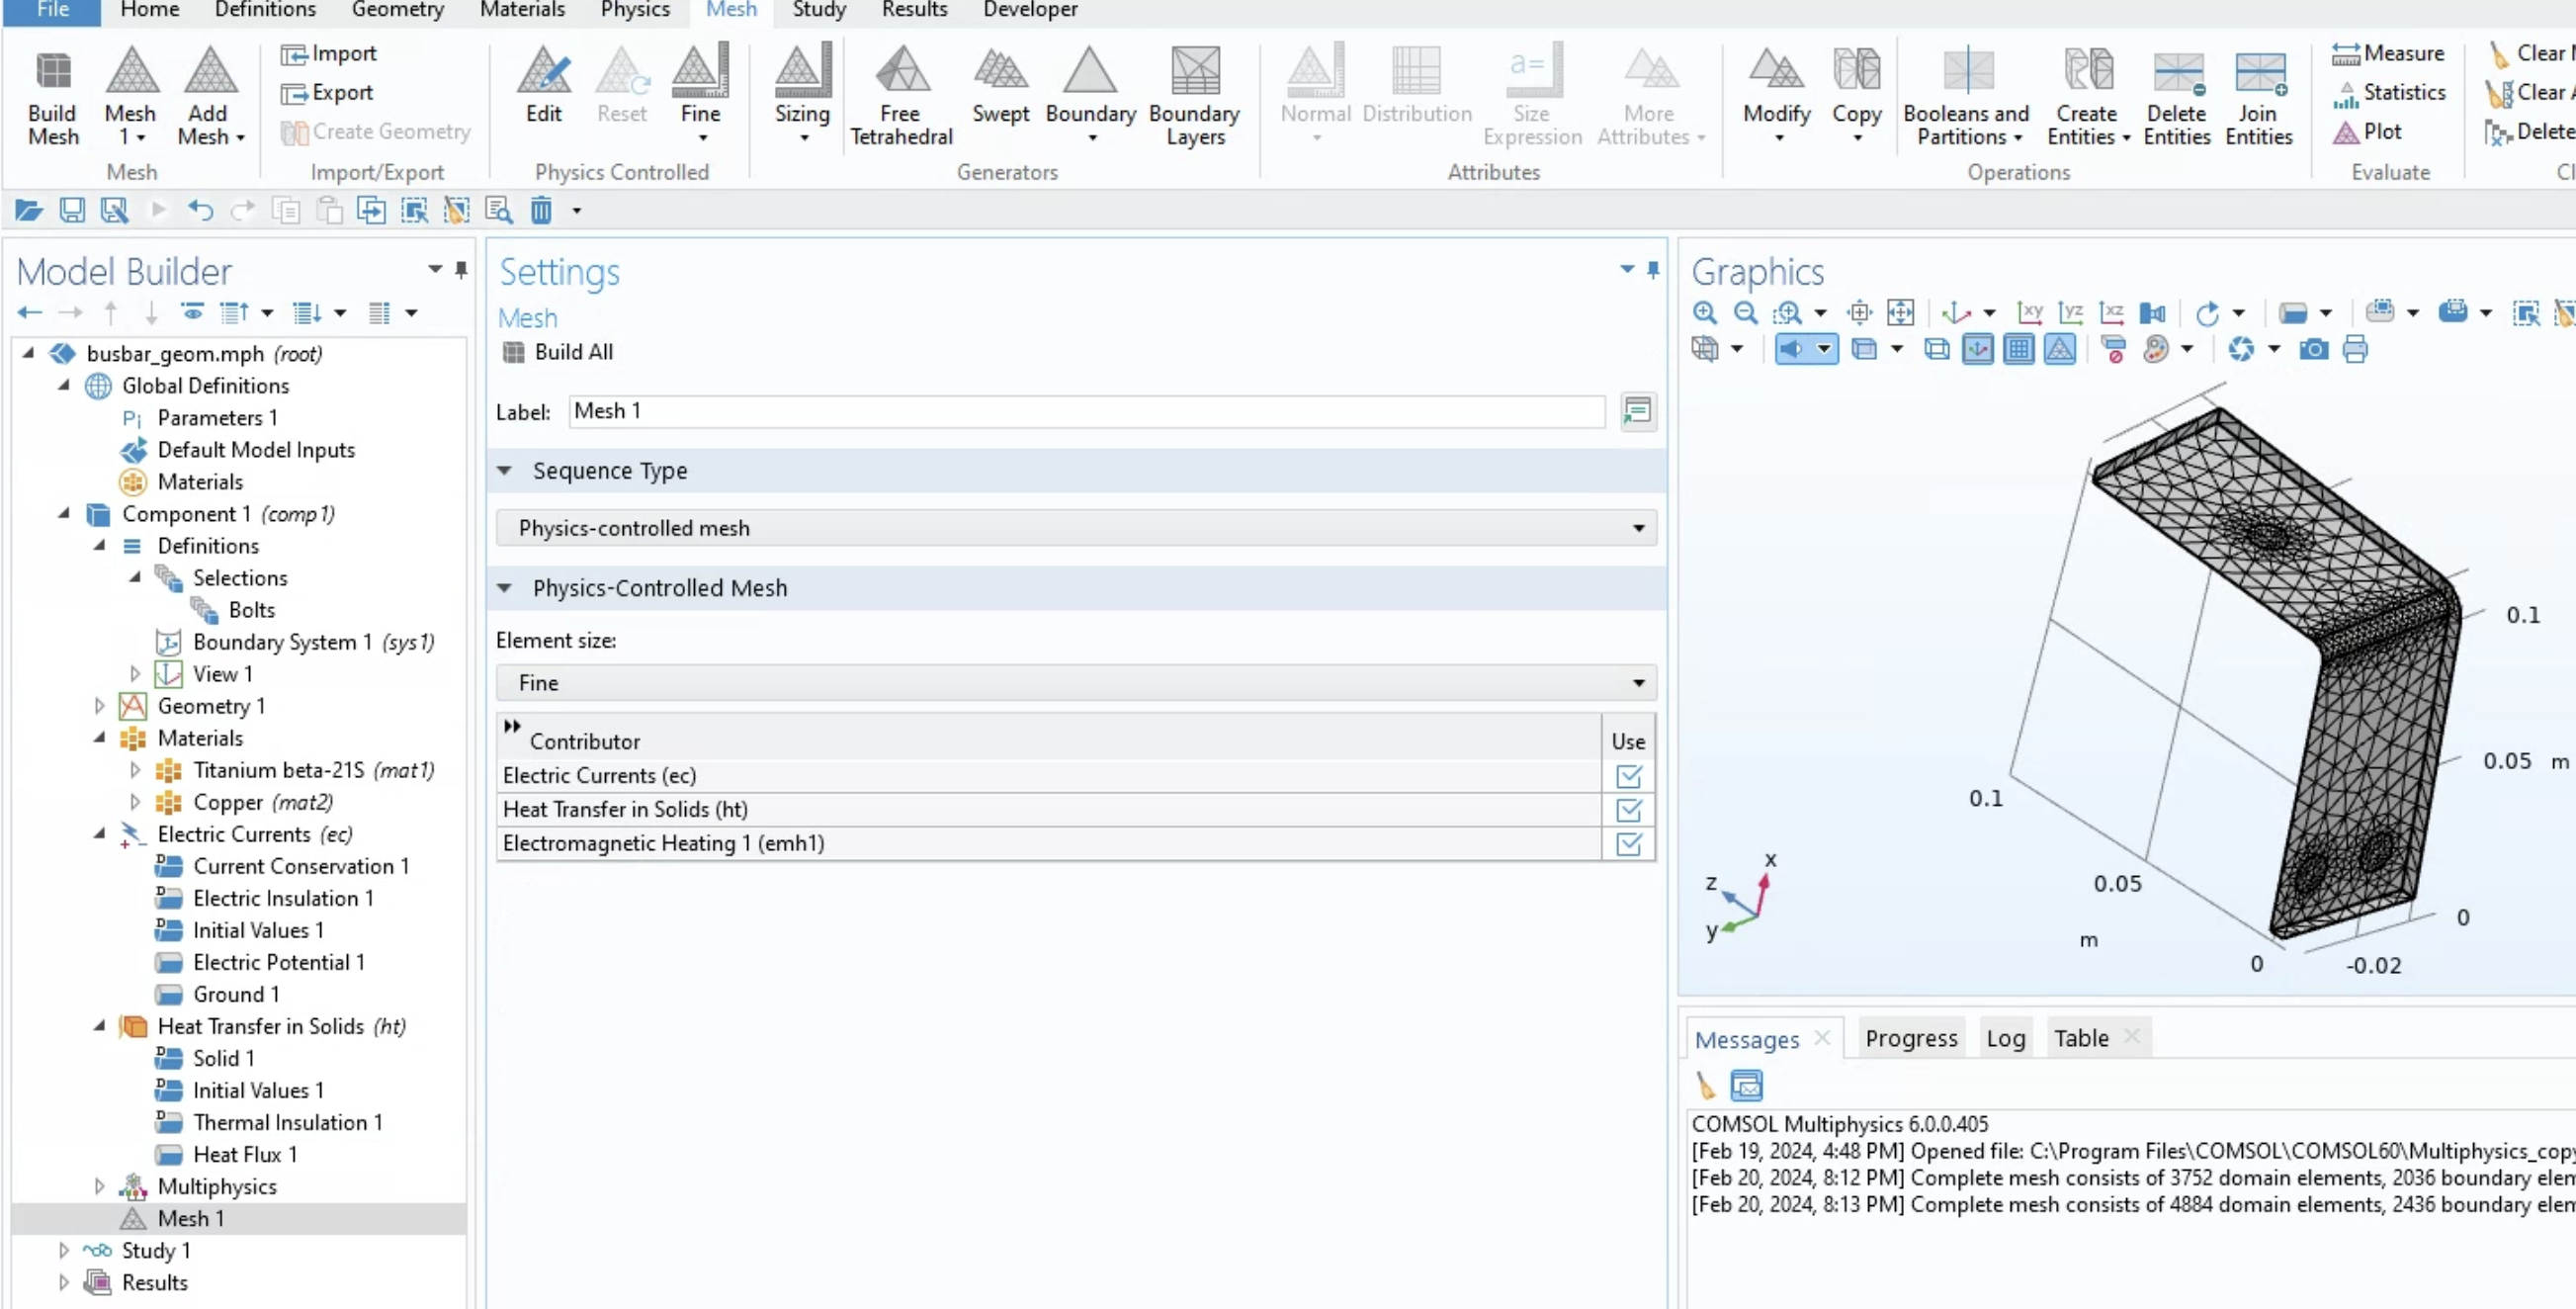
\includegraphics[width=0.4\textwidth]{Chapters/Figures/Chapter 3 Figures/Fine Mesh.png}
  \caption{Source: \cite{}}
  \label{}
\end{figure}

% SUBSECTION --- Run the Study ---
\subsection{Run the Study}.
By selecting and expanding the ``Study 1'' node within the Settings, there's an option to ``Generate default plots'', which automatically creates visual representations tailored to the physics defined in the model. Given our focus on electric currents and heat transfer, this function will produce plots detailing both the electric potential and the temperature distribution within the busbar.

Under the ``Step 1: Stationary'' sub-node, found in the ``Physics and Variables'' dropdown, the integration of the multiphysics problem within the ``Solve For'' section becomes visible. Proceed by clicking the ``Compute'' button to perform the simulation. Once computation is complete, the process advances to the next phase, which involves the post-processing of the generated results.

% TODO: Add image showing computed results.
\begin{figure}[ht!]
  \centering
  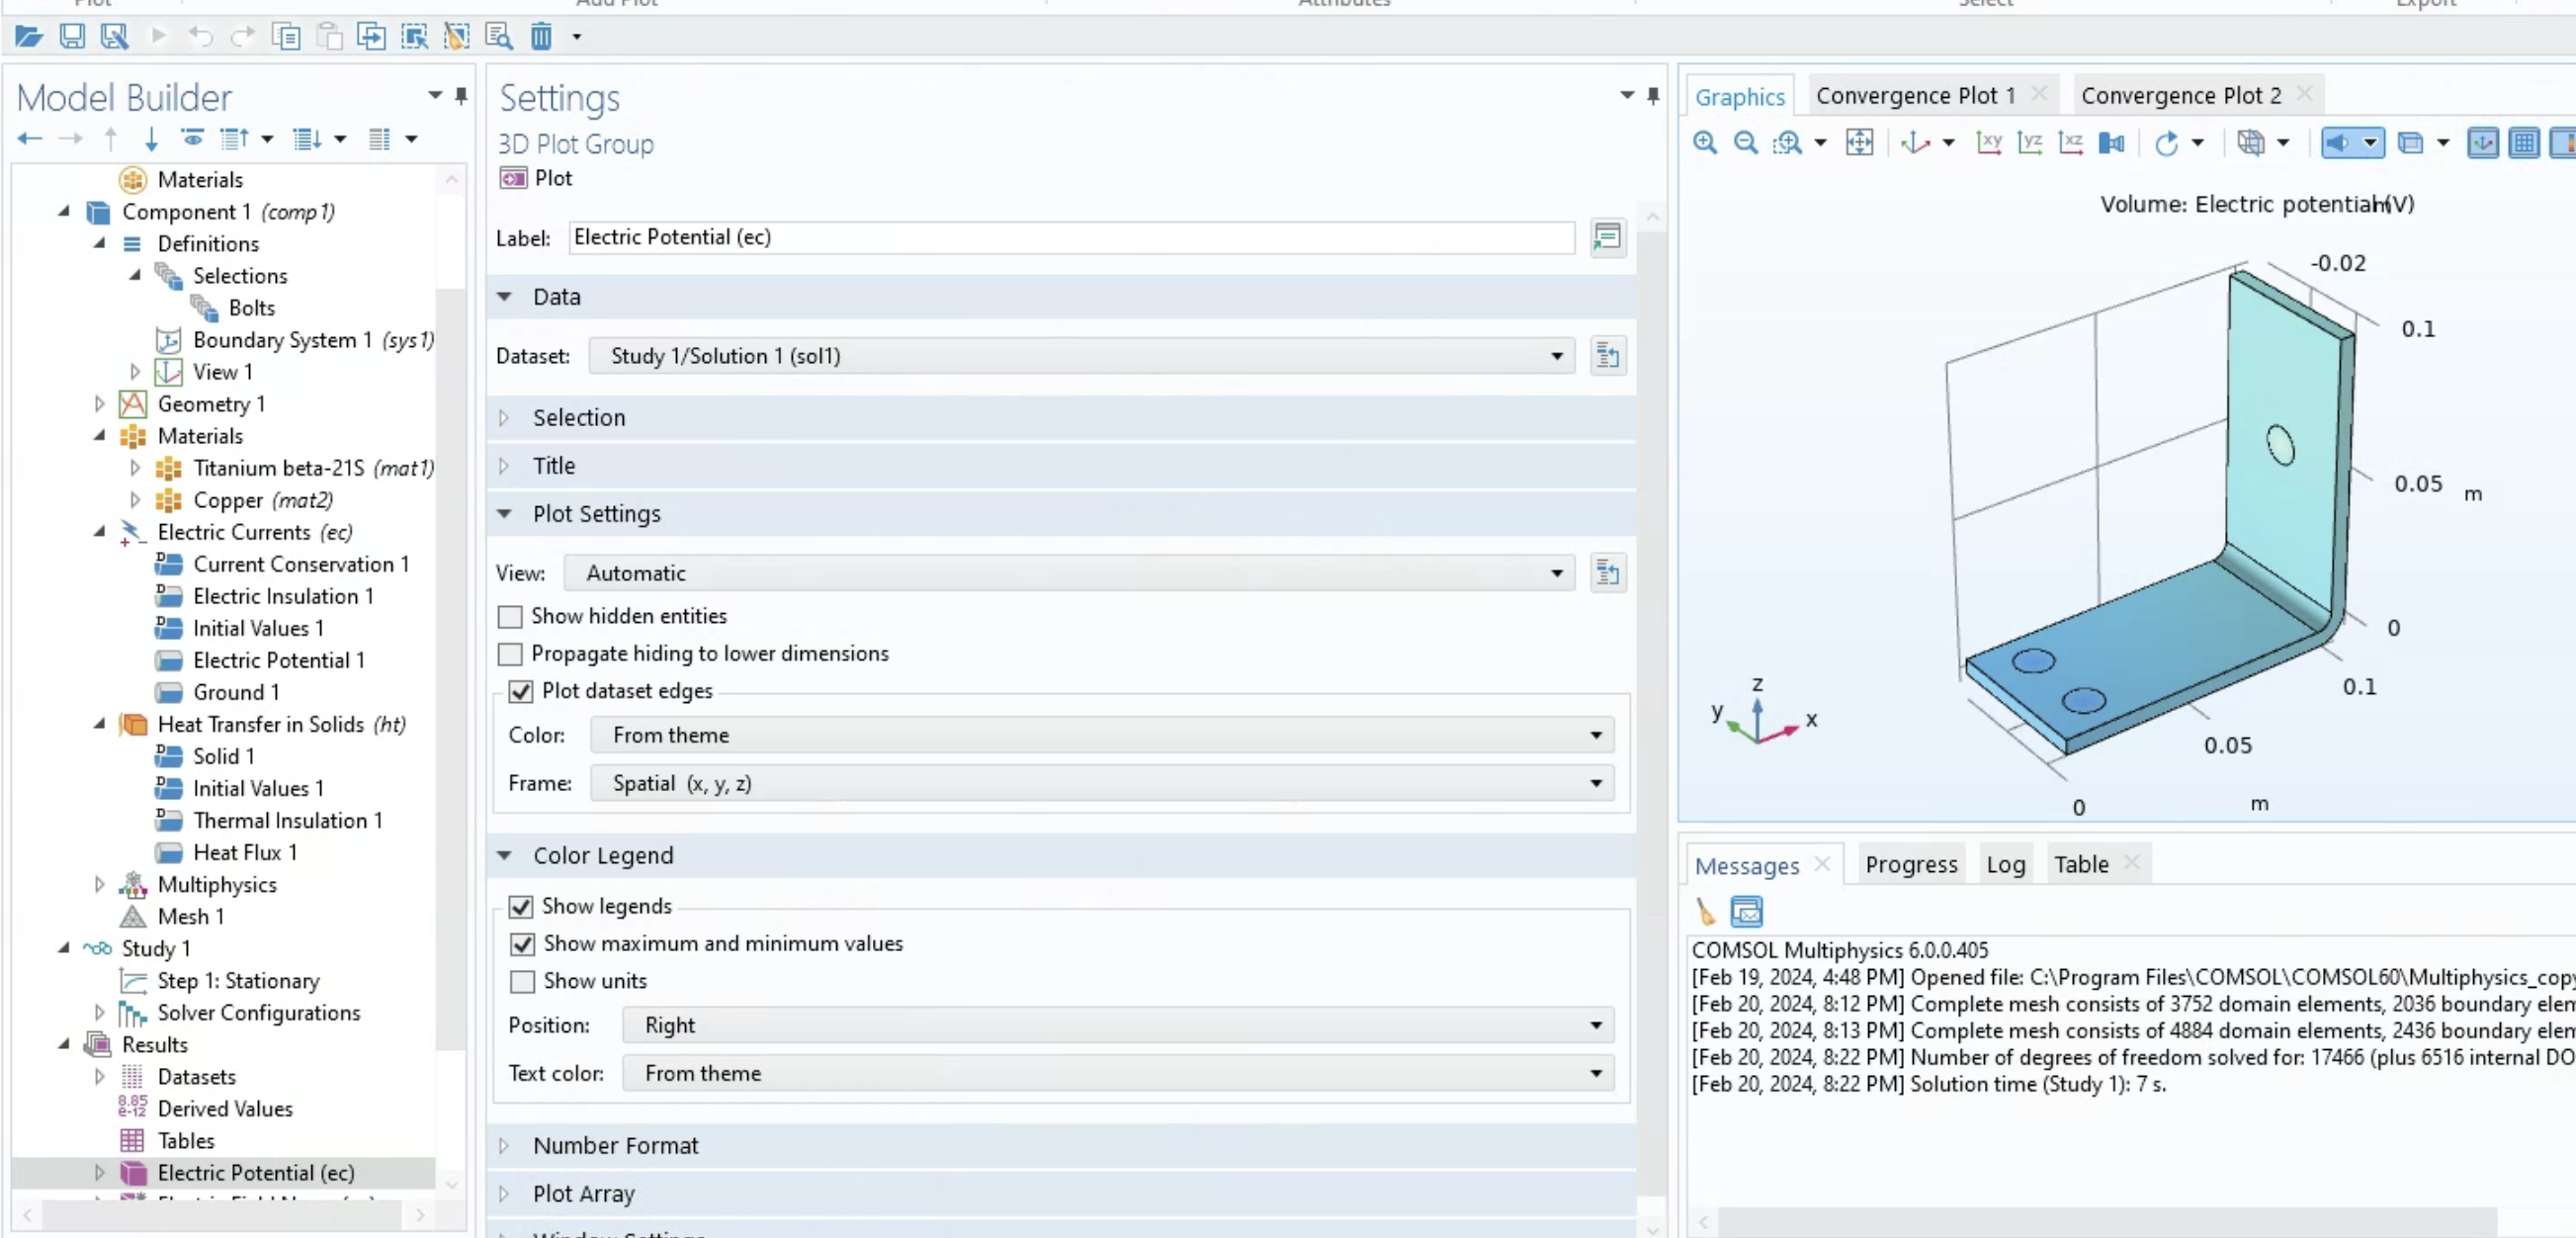
\includegraphics[width=0.4\textwidth]{Chapters/Figures/Chapter 3 Figures/Computed Results.png}
  \caption{Source: \cite{}}
  \label{}
\end{figure}

% SUBSECTION --- Post-Processing the Results ---
\subsection{Post-Processing the Results}.
Upon finalizing the model construction process, the next step involves encapsulating it into a simulation application, achievable via the Application Builder. This tool enables the transformation of the busbar model into an interactive application, providing the flexibility to manipulate specific parameter values.

The Application Builder is readily accessible from the home toolbar.

% TODO: Add image showing application builder button
\begin{figure}[ht!]
  \centering
  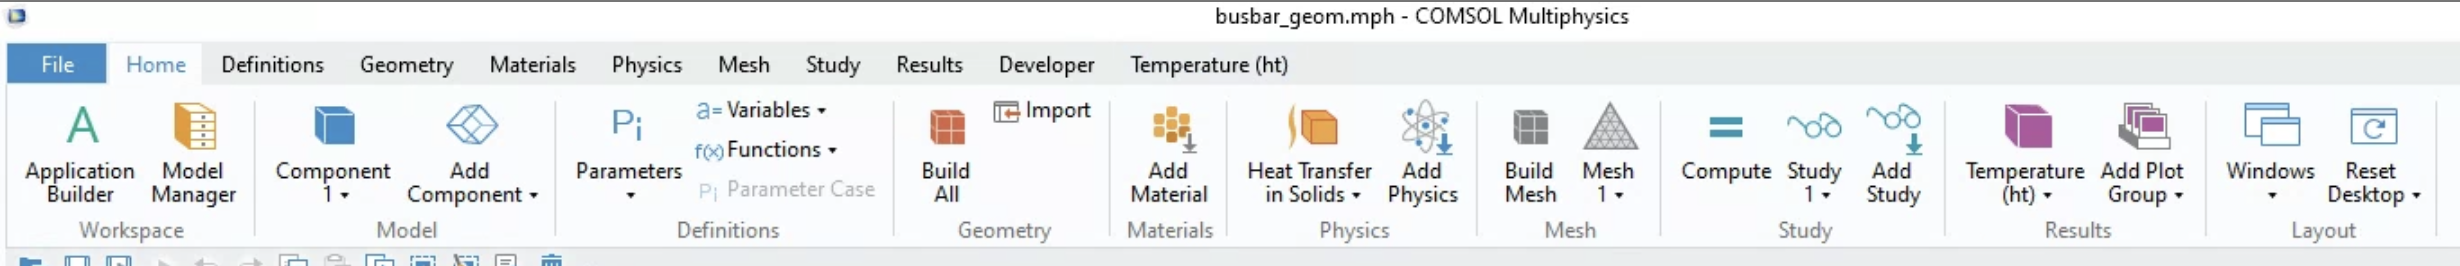
\includegraphics[width=0.4\textwidth]{Chapters/Figures/Chapter 3 Figures/Application Builder Button.png}
  \caption{Source: \cite{}}
  \label{}
\end{figure}

The quick and easy way to create an app is to use the New Form Wizard.

% TODO: Add image showing New Form Wizard button
\begin{figure}[ht!]
  \centering
  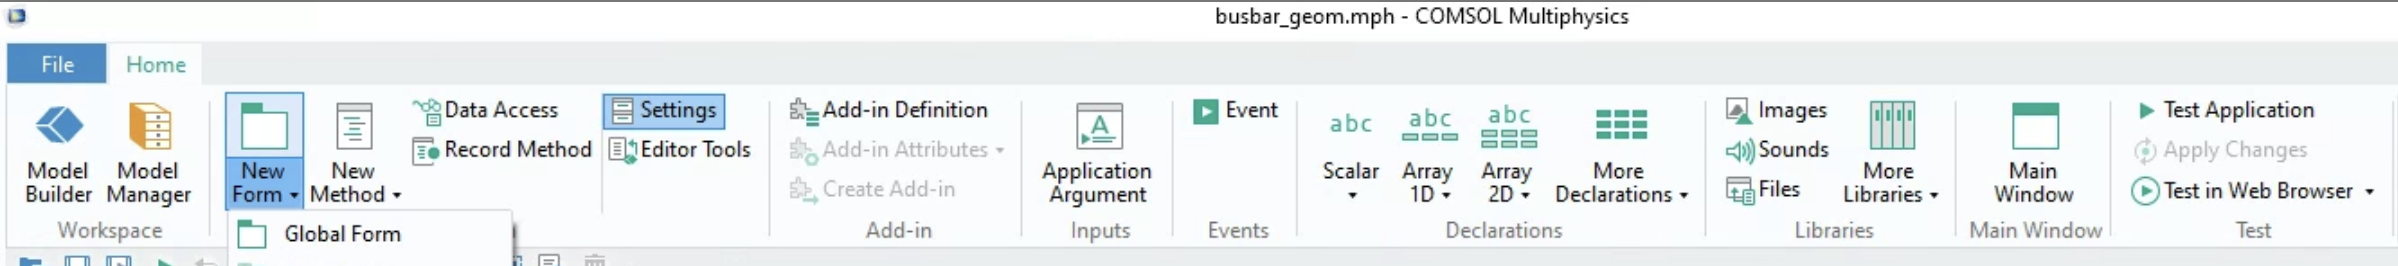
\includegraphics[width=0.4\textwidth]{Chapters/Figures/Chapter 3 Figures/New Form Wizard Button.png}
  \caption{Source: \cite{}}
  \label{}
\end{figure}

From our model, we select parameters whose values can be adjusted, serving as input variables for our simulation application. We opt for the busbar's length, width, and applied voltage as these inputs. Following this, we move to the graphics tab to specify which visuals will be shown in the app. In the subsequent Buttons tab, it's crucial to add the ``Compute Study'' button to initiate simulations.

Upon clicking ``Done'', the Form Editor is launched, allowing us to refine the app's user interface. This includes customizing its look, structuring the display through various forms, and implementing methods to extend its functionality significantly.

% TODO: Add image showing Form Editor
\begin{figure}[ht!]
  \centering
  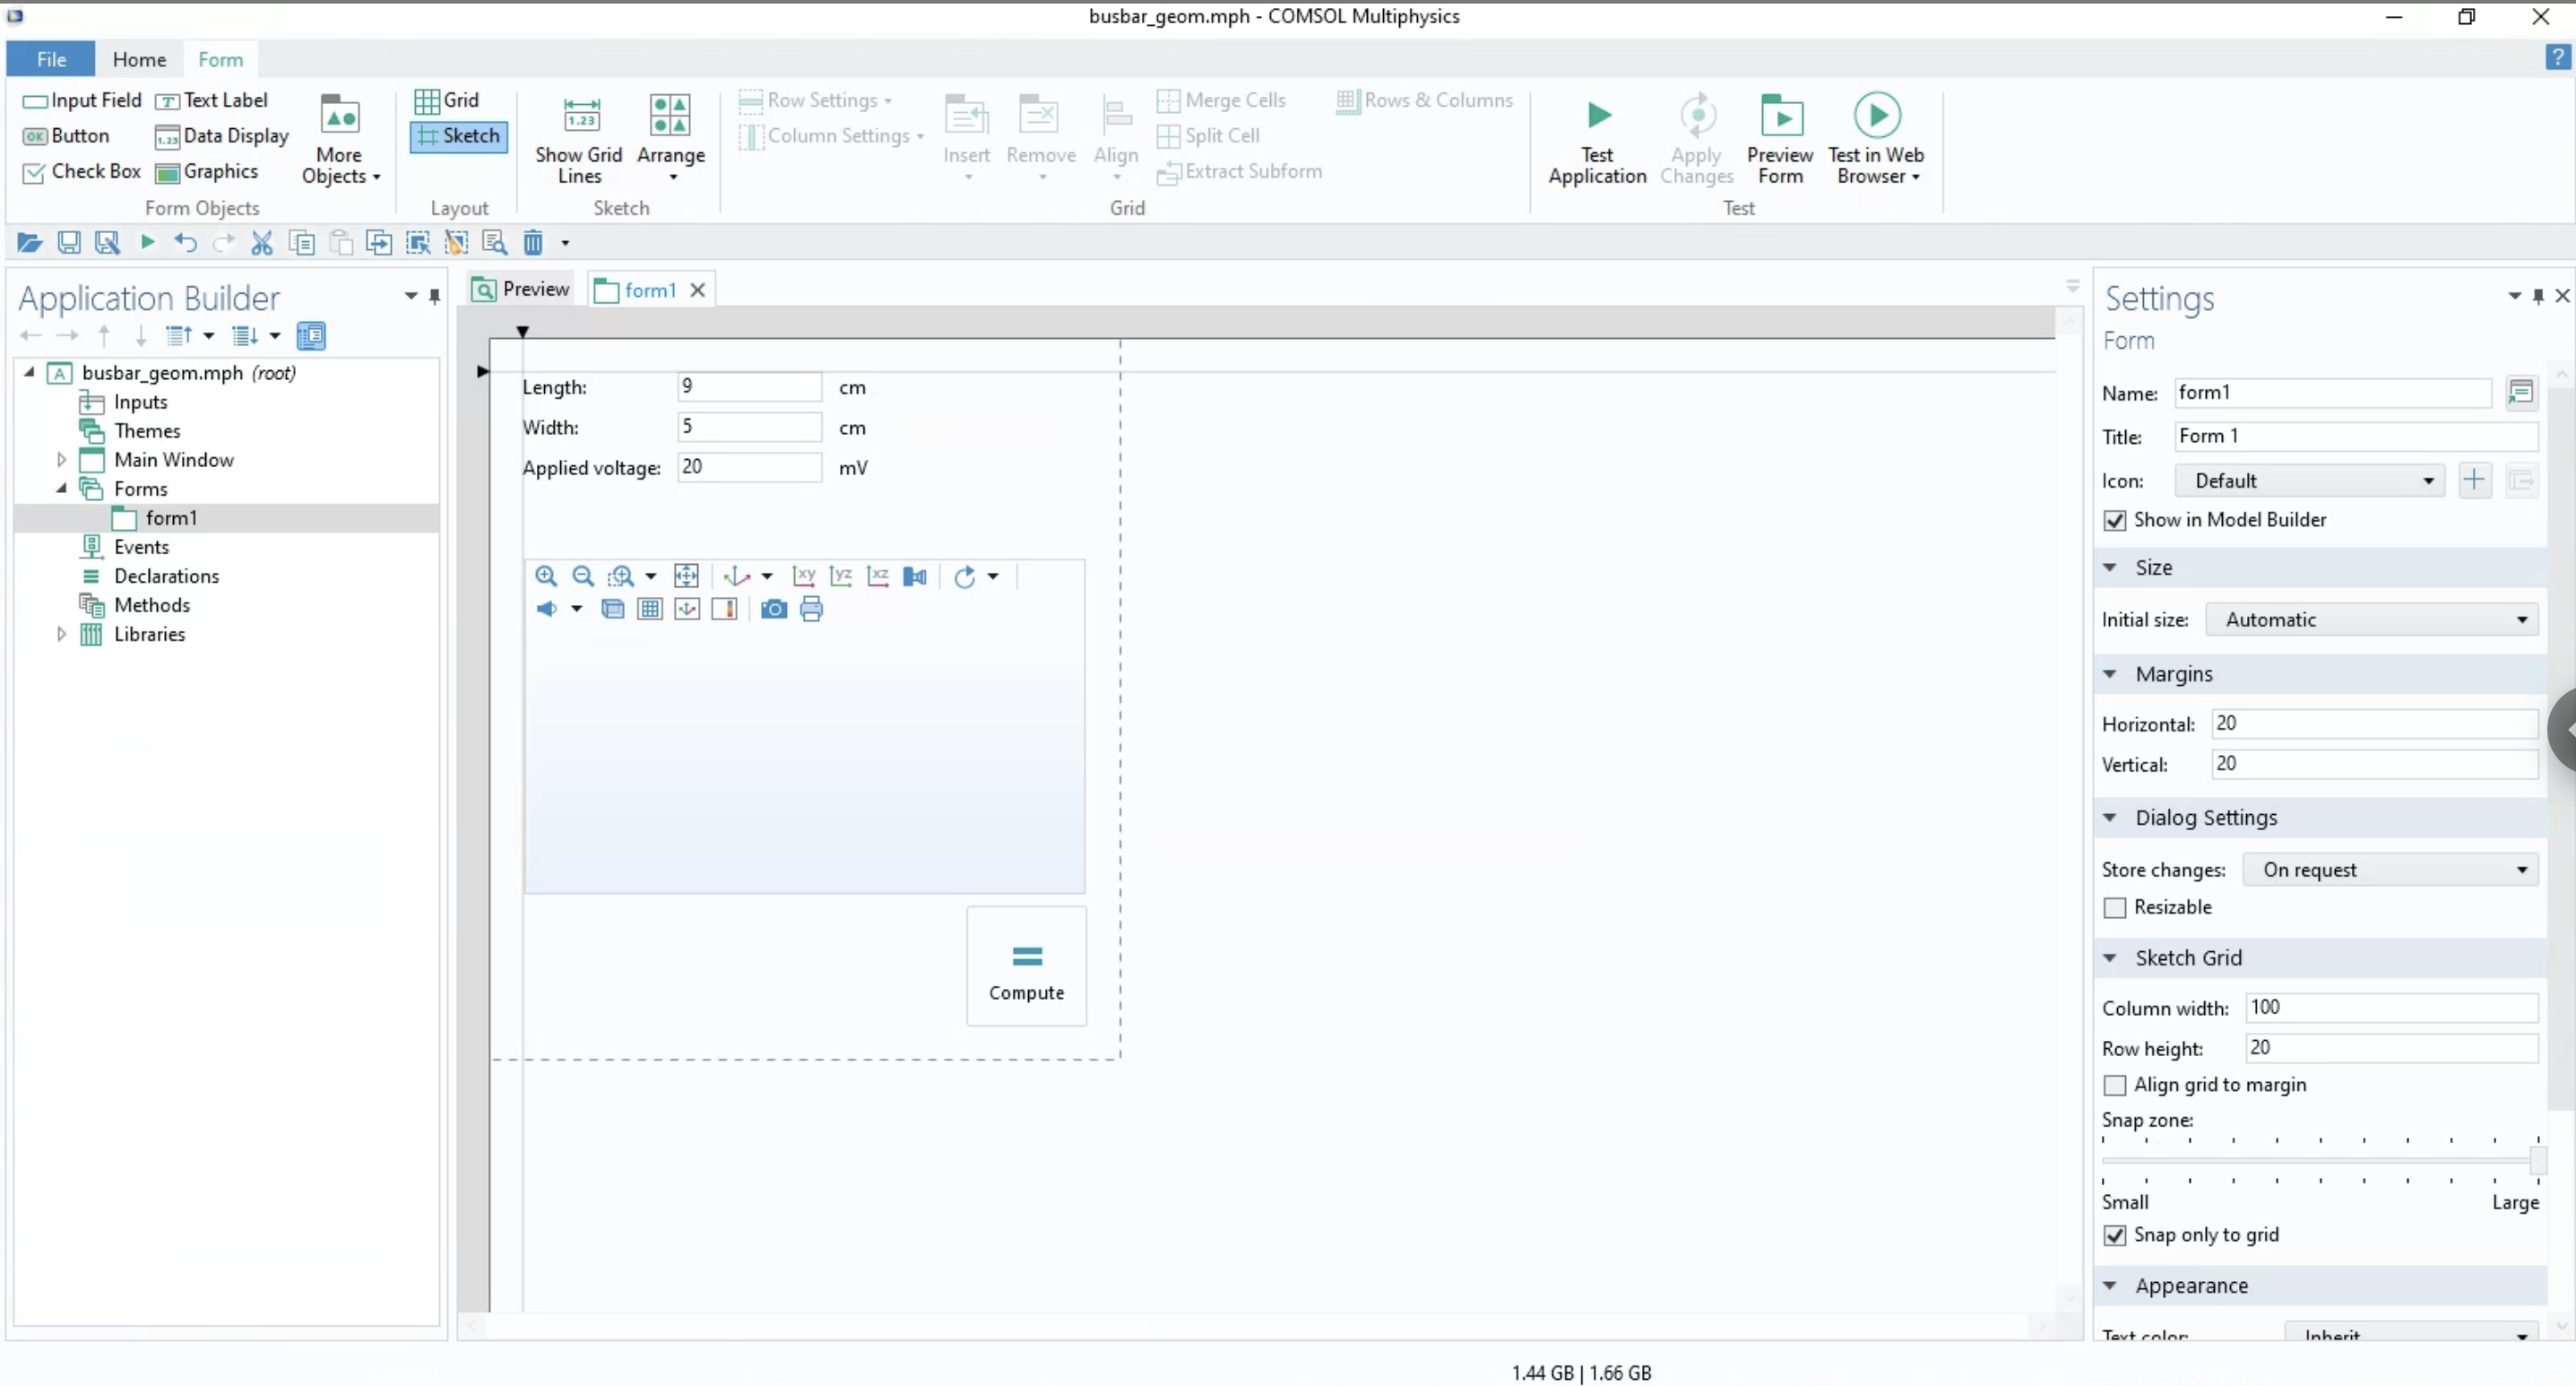
\includegraphics[width=0.4\textwidth]{Chapters/Figures/Chapter 3 Figures/Form Editor Desktop.png}
  \caption{Source: \cite{}}
  \label{}
\end{figure}

If we click the Test Application button, our simulation app appears.

% TODO: Add image after clicking "Test Application" button
\begin{figure}[ht!]
  \centering
  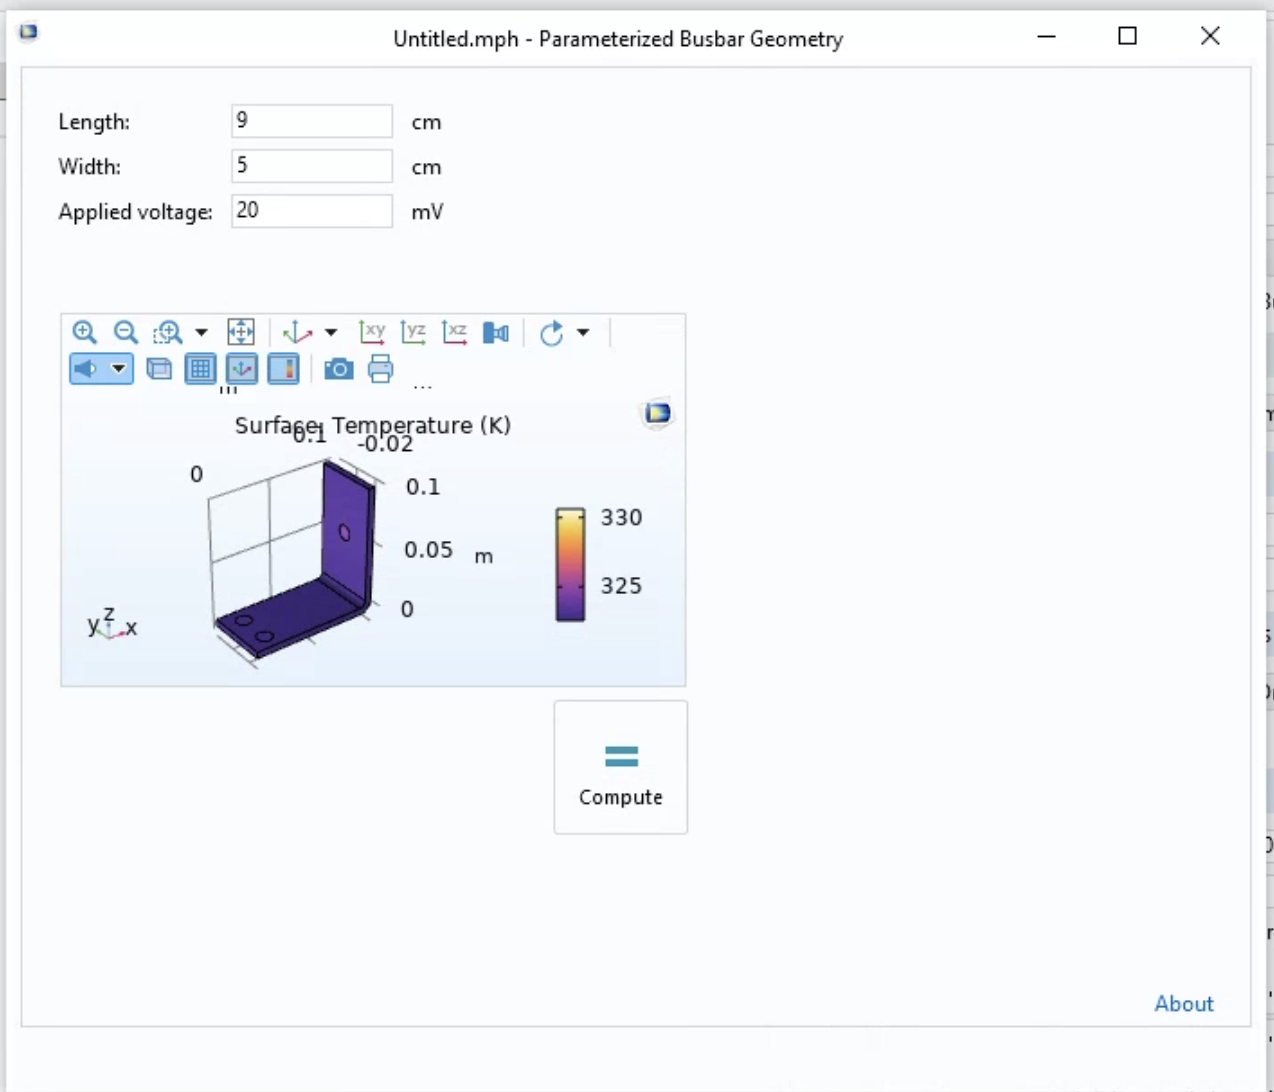
\includegraphics[width=0.4\textwidth]{Chapters/Figures/Chapter 3 Figures/Test Application Results.png}
  \caption{Source: \cite{}}
  \label{}
\end{figure}

We can change some of the values of the parameters such as increasing the length and the width and re-run the app by clicking ``Compute''.

%-----------------HERE------------

\chapter{Computational Results}
Embarking on the findings of this chapter, I transition from the established COMSOL modeling workflow to the critical stage of validating theoretical concepts through the lens of computational analysis. The essence of this chapter is twofold: first, to harness the computational prowess of COMSOL in validating key optical phenomena such as anti-reflectivity thus corroborate our simulation outcomes with theoretical models; and second, to attempt to model the simplest Passive Daytime Radiative Cooling devices (PDRCs) at Hudgings Lab by showing how their reflectance varies with wavelength.

My investigation begins with an empirical analysis of anti-reflective behaviors, examining both simple and composite multilayer arrangements. These simulations are meticulously compared to the theoretical predictions presented in \emph{Introduction to Optics} by Frank L. Pedrotti et al. \cite{pedrotti_introduction_2007}.

It is crucial to acknowledge—as delineated in Chapter 2—the analytical derivation of reflectance as a function of angle $R(\theta)$ and wavelength $R(\lambda)$ is straightforward for materials with a constant refractive index $n$. However, the complexity escalates when dealing with materials where the refractive index varies with $\lambda$, a common occurrence in real-world applications. This variation poses significant challenges to traditional analytical methods, thereby necessitating the adoption of sophisticated computational tools like COMSOL for accurate simulations.

We delve into the intricacies of high reflectance by simulating stacks of alternating high and low refractive index layers, shedding light on the nuanced ways layer configurations impact reflectance. These insights are bench-marked against scholarly literature, reinforcing the accuracy of our models.

Moreover, the thesis explores the layered design of PDRCs. By systematically layering silicon, silver, and Polydimethylsiloxane (PDMS), we dissect the optical properties crucial to the development of passive cooling systems. The collection of results and graphs here encapsulate more than just data; they are catalysts for continuous inquiry and deeper understanding of optical physics as it related to PDRCs.

% ---------- SECTION: COMSOL: MODELING ANTI-REFLECTANCE COATINGS ----------

\section{COMSOL: Modeling Anti-Reflectance Coatings}

As we progress in our exploration of anti-reflectance coatings, it is beneficial to revisit the foundational principles that govern their behavior. These coatings are designed to minimize reflection and maximize transmission of light through strategic manipulation of refractive indices across different layers.

To appreciate the mathematical underpinnings of these designs, recall a pivotal formula, Equation \ref{reflectance for 2-layer antireflecting films}, that encapsulates the essence of a two-layer anti-reflecting film's performance. Assuming light strikes normally on the film, the reflectance, $R$, can be described by the following relationship:

\begin{equation}\label{reflectance for 2-layer antireflecting films - chap4}
    R = \left(\frac{n_0n_2^2 - n_sn_1^2}{n_0n_2^2 + n_sn_1^2}\right)^2
\end{equation}

Here, we anticipate zero reflectance when the expression in the numerator becomes zero, leading us to equation \ref{zero reflectance criterion}, which stipulates the condition for achieving no reflectance:

\begin{equation}\label{zero reflectance criterion - chap4}
    \frac{n_2}{n_1} = \sqrt{\frac{n_s}{n_0}}
\end{equation}

This relationship delineates the necessary ratio between the refractive indices of the layers that leads to a reflectance of zero.

When working with a glass substrate of refractive index $n_s = 1.5$ and air of refractive index $n_0 = 1$, the ideal refractive index ratio, $\frac{n_2}{n_1}$, is calculated to be $\sqrt{1.5} \approx 1.225$.

In COMSOL, our goal is to identify and define (in our parameters table) two materials for the double-layer structure that closely match this ratio to maximize anti-reflective properties. It is crucial to note that the refractive index of most materials varies with wavelength. This variability, known as dispersion, means that optimal thickness and refractive indices for minimizing reflectance at one wavelength may not be as effective at another. While it is challenging to select materials that precisely align their refractive indices to achieve exactly zero reflectance, our aim is to get as close to 0\% reflectance over as wide a $\lambda$ range as practically possible.

The limitation of a quarter-wavelength layer is its selective reflectivity; it effectively eliminates reflection at a specific wavelength but substantially reflects at other wavelengths in proximity. Additionally, its performance varies significantly with the angle at which light strikes the surface. A viable solution to overcome this is the application of multilayer coatings. These coatings, compared to their single-layer counterparts, tend to lower the reflection coefficient over a broader spectrum and accommodate a greater diversity of tangible materials \cite{pedrotti_introduction_2007}.

In the following section, we will compare the reflectivity of two distinct multilayer coatings across an extensive spectral range. The analysis will cover a dual-layer (quarter-quarter wavelength coating) and a triple-layer (quarter-half-quarter wavelength coating). It will be demonstrated that the triple-layer coating achieves a more uniform low reflectance throughout the majority of the visible light spectrum.

% ---------- SUBSECTION: ANTI-REFLECTANCE LAYERS: SETUP ----------

\subsection{Anti-reflectance Layers: Setup}

The pursuit of anti-reflective coatings leads us to the utilization of thin film dielectrics within COMSOL. In line with the criteria for zero reflectance, the first dielectric film, starting from the base, is cerium trifluoride ($\text{CeF}_3$) with a refractive index of 1.63, while the second film is magnesium fluoride ($\text{MgF}_2$) with a refractive index of 1.38. The refractive index ratio of approximately 1.181 aligns closely with the optimal ratio of 1.225. As established in chapter 2, effective anti-reflectivity for a dual-layer arrangement requires each film to be a quarter-wavelength in thickness, which corresponds to the wavelength at which minimal reflectance is desired.

\begin{figure}[H]
  \centering
  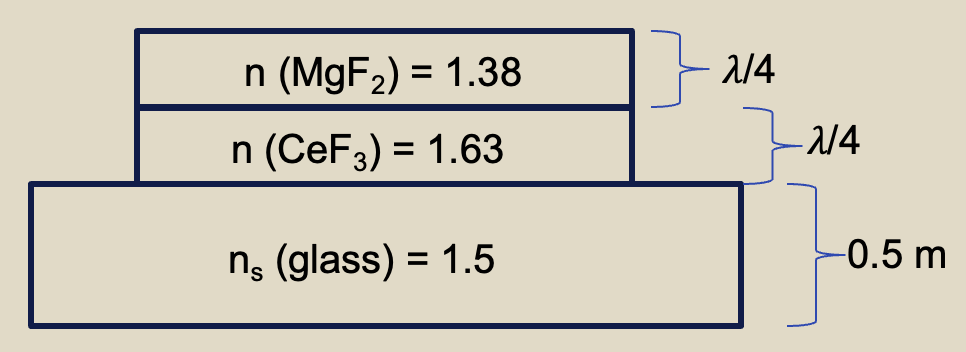
\includegraphics[width=0.7\textwidth]{Chapters/Figures/Chapter 4 Figures/Antireflective Double-Layer (PowerPoint).png}
  \caption{The double-layer anti-reflectance coating layout (dimensions not to scale). Source: created by the author using Microsoft PowerPoint.}
  \label{fig:Antireflective Double-Layer (PowerPoint)}
\end{figure}

In our enhanced three-layer structure, designed to broaden anti-reflectivity across a larger wavelength spectrum, the middle layer is a half-wavelength film of zirconium dioxide ($\text{ZrO}_2$), chosen for its refractive index of 2.2. This multi-layer configuration allows for increased anti-reflective performance compared to the more wavelength-specific two-layer model.

\begin{figure}[H]
  \centering
  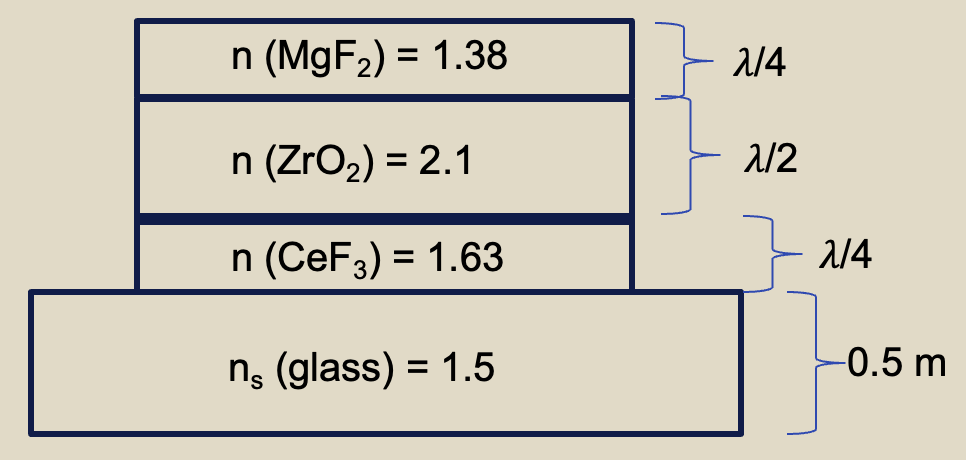
\includegraphics[width=0.7\textwidth]{Chapters/Figures/Chapter 4 Figures/Antireflective Triple-Layer (PowerPoint).png}
  \caption{The triple-layer anti-reflectance coating layout (dimensions not to scale). Source: created by the author using Microsoft PowerPoint.}
  \label{fig:Antireflective Triple-Layer (PowerPoint)}
\end{figure}

This screenshot from the COMSOL desktop highlights the configuration for modeling anti-reflective coatings. Pay particular attention to the 'Film Properties' area within the 'Thin Dielectric Film' settings where the quarter-wavelength calculation is outlined.

\begin{figure}[H]
  \centering
  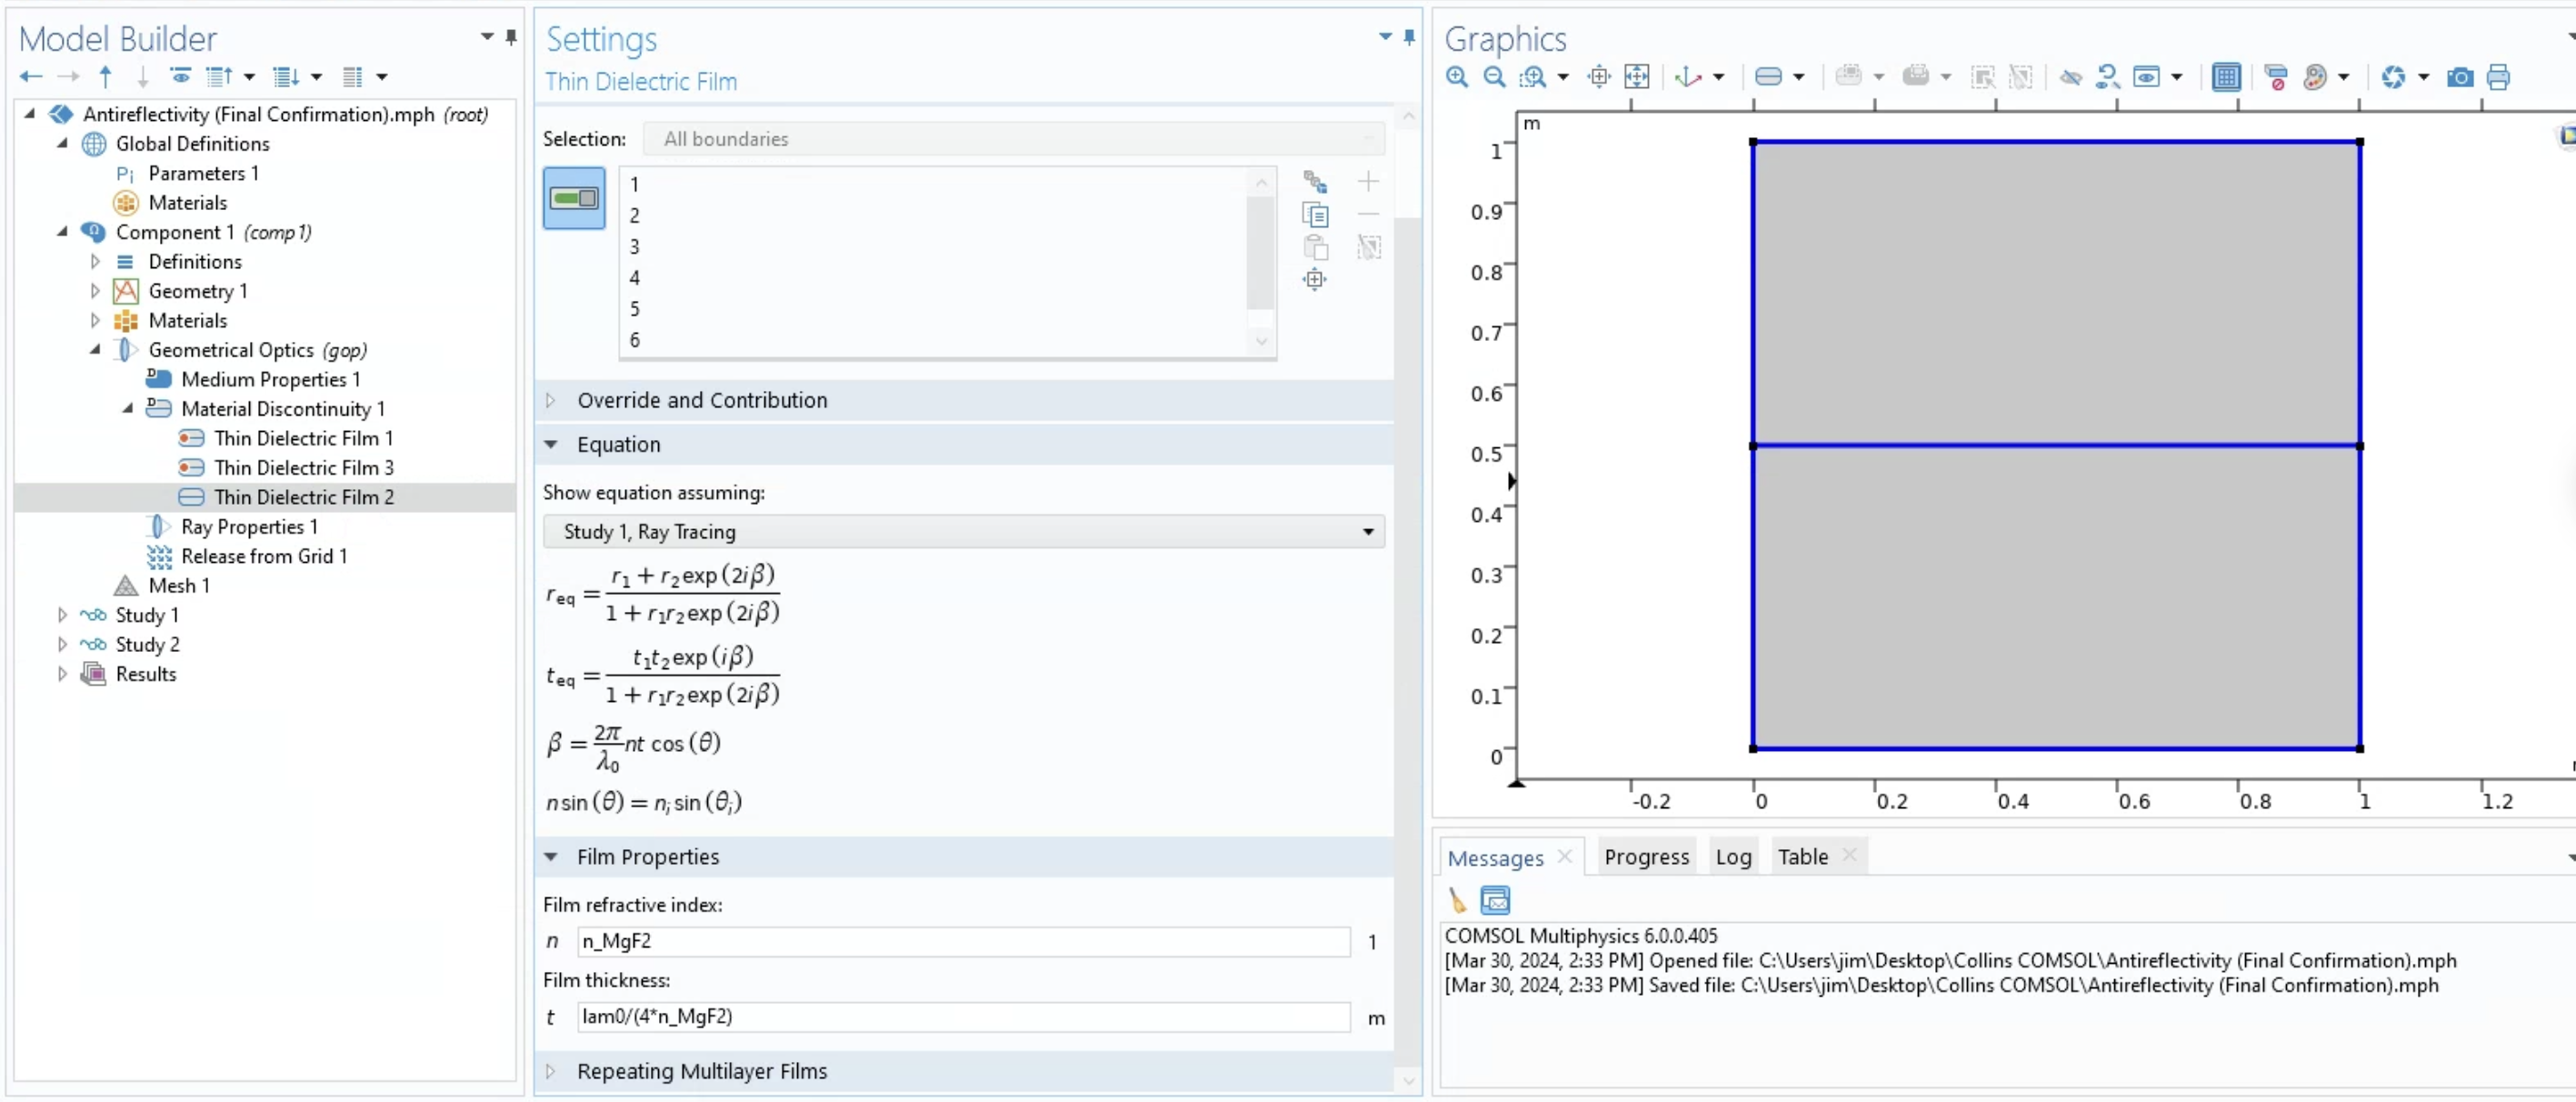
\includegraphics[width=0.7\textwidth]{Chapters/Figures/Chapter 4 Figures/COMSOL Desktop Showcasing Antireflectivity Setup.png}
  \caption{COMSOL desktop setup showcasing anti-reflectivity modeling.}
  \label{fig:COMSOL desktop showcasing antireflectivity}
\end{figure}

Here, the findings from the anti-reflectivity modeling using $\text{CeF}_3$ and $\text{MgF}_2$ for the quarter-quarter wavelength combination, as well as $\text{CeF}_3$, $\text{MgF}_2$, and $\text{ZrO}_2$ for the quarter-half-quarter wavelength setup, are presented.

\begin{figure}[H]
  \centering
  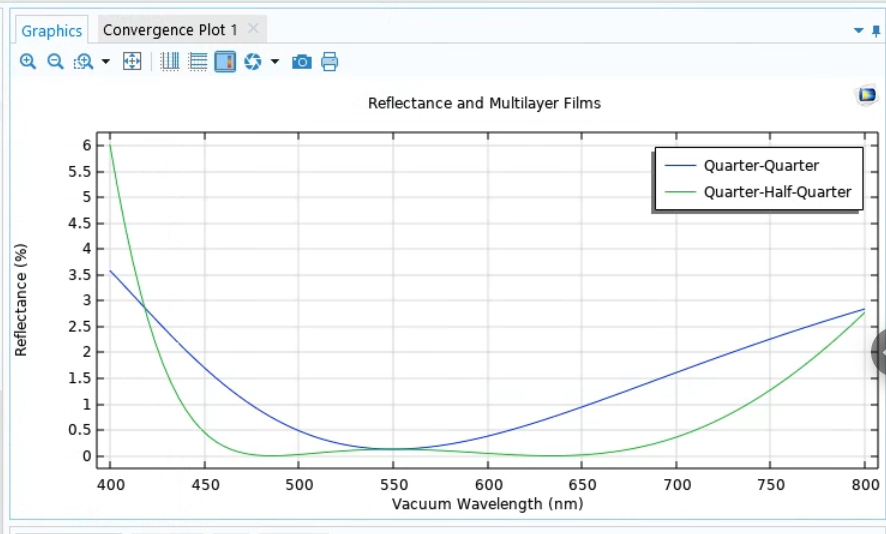
\includegraphics[width=0.7\textwidth]{Chapters/Figures/Chapter 4 Figures/Quarter-Half-Quarter.png}
  \caption{Illustration of the reflectance behavior for two anti-reflective coating configurations across the visible light spectrum. The blue line indicates the performance of a quarter-quarter wavelength coating, whereas the green line shows the effect of a quarter-half-quarter wavelength coating.}
  \label{fig:both quarter-quarter and quarter-half-quarter}
\end{figure}

In the quarter-quarter wavelength design, we employ two layers, each precisely a quarter of the desired wavelength in thickness. While the aim is to achieve minimal reflectance at a particular wavelength, the actual reflectance seldom reaches absolute zero due to the inherent limitations of material characteristics.

On the other hand, the quarter-half-quarter arrangement introduces an additional layer, half a wavelength thick, nestled between two quarter-wavelength films. This configuration is tailored to minimize reflectance across an extended spectrum of wavelengths.

Such multi-layered coatings surpass the effectiveness of single-layer films for anti-reflective purposes by accommodating a wider wavelength range. This versatility is particularly beneficial in applications where reducing reflection is paramount, such as in the manufacturing of optical lenses.

% ---------- SUBSECTION: VERIFYING ANTI-REFLECTANCE COMPUTATIONAL RESULTS THROUGH COMPARISON WITH THEORETICAL OPTICS LITERATURE ----------

\subsection{Verifying Anti-Reflectance Computational Results Through Comparison with Theoretical Optics Literature}

This section aims to validate the obtained computational results with the principles outlined in \emph{Introduction to Optics} by Frank L. Pedrotti et al \cite{pedrotti_introduction_2007}.

Beginning with a straightforward approach, we examine the reflectance across various wavelengths for three distinct multilayer film configurations:
\begin{enumerate}
    \item Films with quarter-quarter wavelength thickness.
    \item Films with quarter-half wavelength thickness.
    \item Films with quarter-half wavelength thickness, incorporating a different material for the half-wavelength layer.
\end{enumerate}

\begin{figure}[H]
  \centering
  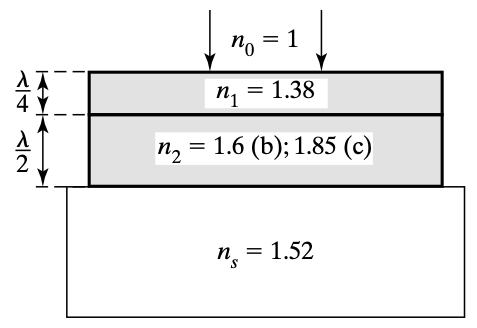
\includegraphics[width=0.7\textwidth]{Chapters/Figures/Chapter 4 Figures/Antireflecting Double Layer using Quarter and Half-Wavelength Thickness Films Layout.png}
  \caption{Antireflective double-layer arrangement. Source: \cite{pedrotti_introduction_2007}}
  \label{fig:antireflective_double_layer}
\end{figure}

We first examine films with quarter-quarter wavelength thickness. The reference from Pedrotti et al. specifies the lower thin dielectric layer as $\text{ZrO}_2$ and places $\text{CeF}_3$ directly above. The choice of materials is flexible, provided they adhere to the optimal ratio criterion for anti reflectance as defined in equation \ref{zero reflectance criterion - chap4}. This results in a refractive index ratio of $\frac{n_2}{n_1} = \frac{2.1}{1.65} \approx 1.273$, aligning closely with the ideal ratio of approximately 1.225 for normal incidence, given a substrate refractive index ($n_s$) of 1.5.

Expanding the spectrum of low reflectance within the visible region becomes achievable by diverging from the constraint of equal quarter-wavelength ($\lambda/4$) coatings. By integrating a layer of quarter-wavelength thickness as the second layer (considered from the bottom upwards), we attain more extensive zones of diminished reflectance. Consequently, in the scenario of item 2, we employ magnesium fluoride ($\text{MgF}_2$), characterized by a refractive index of 1.38, as the quarter-wavelength thick material. The intermediate half-wavelength layer utilizes aluminum oxide, with a refractive index of 1.60. For item 3, thorium dioxide, featuring a refractive index of 1.85, serves as the material for the half-wavelength thick layer, as noted in \cite{pedrotti_introduction_2007}.

For the specific wavelength of 550 nm, where the thicknesses of the quarter-wavelength ($\lambda/4$) and half-wavelength ($\lambda/2$) layers are calculated, the half-wavelength layer does not influence reflectance. In this case, the double-layer system acts akin to a solitary quarter-wavelength layer, resulting in a reflectance of 1.3\%. At wavelengths close to 550 nm, the presence of the half-wavelength layer contributes to maintaining reflectance levels below those achieved by a two quarter-wavelength layers. Below is the plot illustrating reflectance against wavelength for scenarios 1 through 3.

The graph below illustrates anti-reflectivity trends as detailed in the Optics textbook, indicating that while the reflectance at a wavelength of 550 nm stands at approximately 1.3\%, this value surpasses the performance of the quarter-quarter wavelength coating. Nevertheless, reflectance stays below this threshold across a wide wavelength span, extending from roughly 420 to 800 nm. This suggests that alternative configurations for dual-layer reflective films could be viable if the layers are not strictly constrained to quarter-wavelength multiples.

\begin{figure}[H]
  \centering
  % Top left figure
  \begin{minipage}{0.45\textwidth}
    \centering
    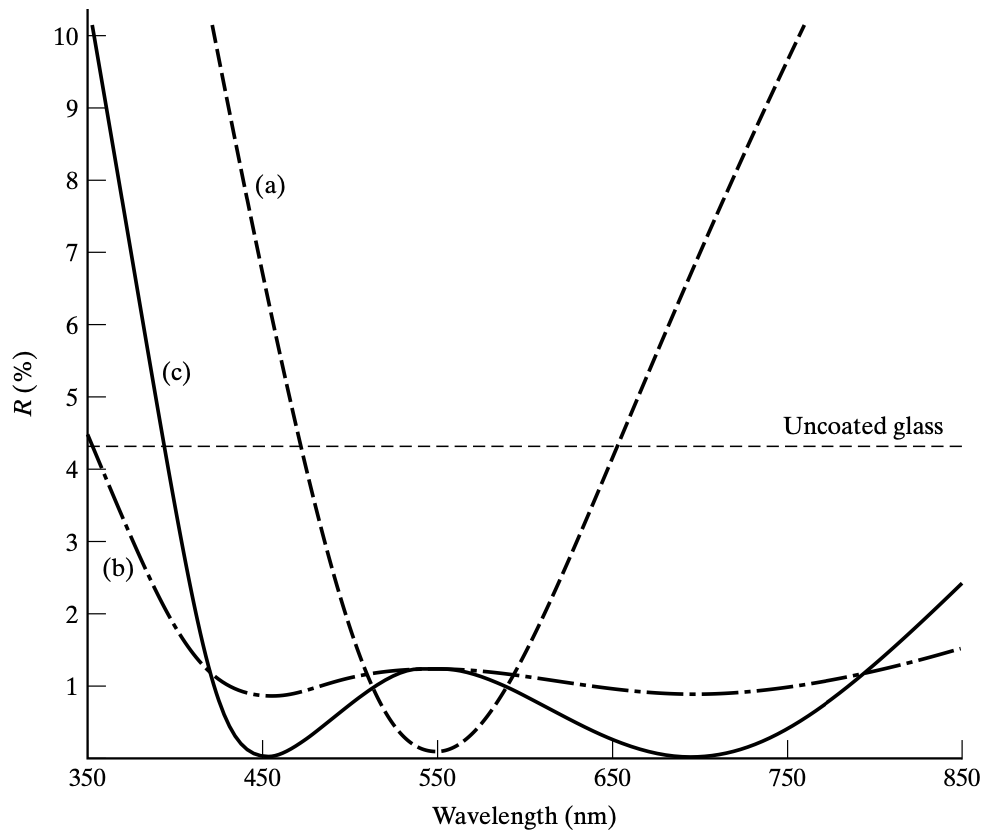
\includegraphics[width=\textwidth]{Chapters/Figures/Chapter 4 Figures/Antireflectivity Graphs in the Optics Book.png}
    \caption{Anti-reflectivity Graphs as shown in the Optics Textbook.}
    \label{fig:antireflectivity graphs in the Optics book}
  \end{minipage}\hfill
  % Top right figure
  \begin{minipage}{0.45\textwidth}
    \centering
    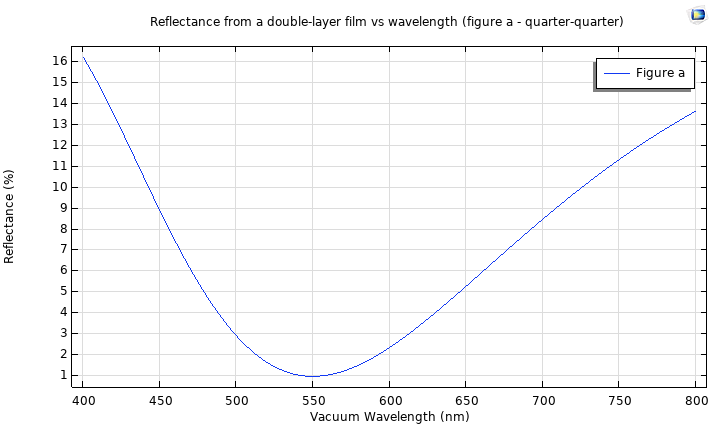
\includegraphics[width=\textwidth]{Chapters/Figures/Chapter 4 Figures/Anti-Reflectance Figure a.png}
    \caption{Modeling results of an anti-reflective coating with two layers, each a quarter-wavelength thick.}
    \label{fig:Antireflective Figure a}
  \end{minipage}
  % Bottom left figure
  \begin{minipage}{0.45\textwidth}
    \centering
    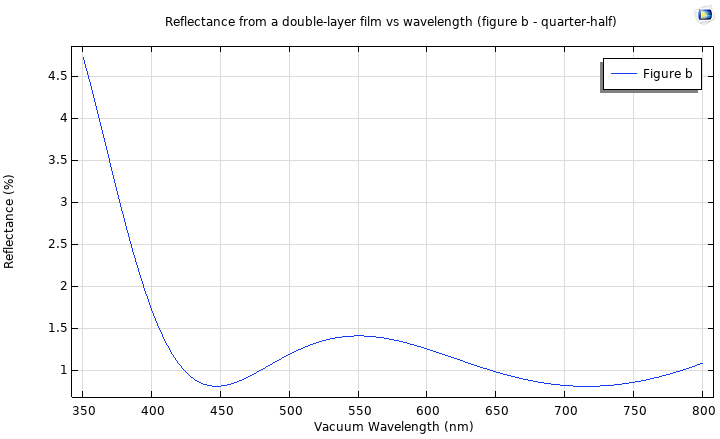
\includegraphics[width=\textwidth]{Chapters/Figures/Chapter 4 Figures/Anti-Reflectance Figure b.png}
    \caption{Reflectance outcomes for an anti-reflective coating with a bottom layer a quarter-wavelength thick and a top layer half-wavelength thick, using a material with a refractive index of 1.6.}
    \label{fig:Antireflective Figure b}
  \end{minipage}\hfill
  % Bottom right figure
  \begin{minipage}{0.45\textwidth}
    \centering
    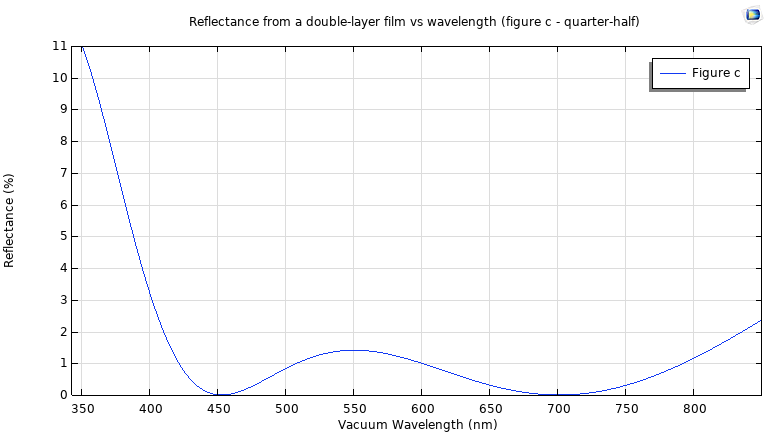
\includegraphics[width=\textwidth]{Chapters/Figures/Chapter 4 Figures/Anti-Reflectance Figure c.png}
    \caption{Reflectance results for an anti-reflective double layer with a bottom layer a quarter-wavelength thick and a top layer half-wavelength thick, using a material with a refractive index of 1.85.}
    \label{fig:Antireflective Figure c}
  \end{minipage}
\end{figure}

These results derive from the principles outlined in Chapter 2. Initially, the overall transfer matrix elements are calculated by multiplying the transfer matrices of the individual layers together. Within these calculations, the phase difference, $\delta$, varies with $\lambda$, aligning the film thickness with either $\lambda/4$ or $\lambda/2$ at the reference wavelength of 550 nm.

Subsequently, the reflection coefficient, as outlined in \ref{reflection coefficient in terms of transfer matrix terms}, is squared to produce reflectance as a wavelength function. COMSOL's Ray Optics module significantly simplifies this process by automating several steps, although careful consideration is needed for layer treatment, particularly regarding their classification as thin dielectric films.

\section{COMSOL: Modeling High Reflectance.}
To achieve anti-reflective properties, layers are arranged starting from the air and progressing through low-index to high-index materials before reaching the substrate. In contrast, for enhanced reflectivity, the sequence is reversed, starting from the air to high-index and then to low-index materials before ending at the substrate. This arrangement encourages multiple reflections of the incident light within the layered structure.

A combination of layers arranged to maximize reflectivity is known as a \emph{dielectric mirror}, \emph{high-reflectance stack}, or \emph{distributed Bragg reflector}. It's important to note that achieving high reflectance across the solar spectrum is a key factor for effective passive daytime radiative cooling, as previously discussed.

\begin{figure}[H]
  \centering
  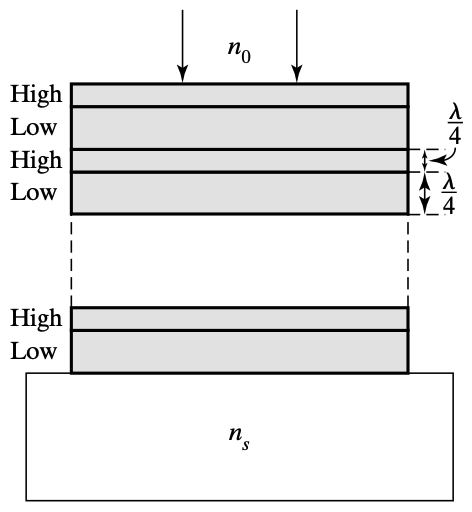
\includegraphics[width=0.5\textwidth]{Chapters/Figures/Chapter 4 Figures/High-Reflectance Stack of Double Layers.png}
  \caption{High-reflectance stack comprising double layers with alternating high and low refractive indices. Source: \cite{pedrotti_introduction_2007}}
  \label{fig:visualizing high-reflectance stack with alternating indices}
\end{figure}

% ---------- SUBSECTION: VERIFYING HIGH REFLECTANCE COMPUTATIONAL RESULTS THROUGH COMPARISON WITH THEORETICAL OPTICS LITERATURE ----------

\subsection{Verifying High Reflectance Computational Results Through Comparison with Theoretical Optics Literature}
The formula to ascertain high reflectance, $R$, at a chosen design wavelength ($\lambda_0$) for a specific layer arrangement is denoted by \ref{maximum reflectance equation}.

\begin{equation}\label{formula for optimal reflectance - chap4}
    R = \left[ \frac{ \left( \frac{n_0}{n_s} \right) \left( \frac{n_L}{n_H} \right)^{2N}  - 1 }{  \left( \frac{n_0}{n_s} \right) \left( \frac{n_L}{n_H} \right)^{2N}  + 1}  \right]^2
\end{equation}

Achieving maximal reflectance (100\%) occurs under the following conditions:
\begin{enumerate}
    \item As $N$, representing the count of layer pairs, becomes very large.
    \item When the ratio $\frac{n_L}{n_H}$ approaches zero.
\end{enumerate}

The optics textbook illustrates high reflectance with the following depiction:

\begin{figure}[H]
  \centering
  % Left figure
  \begin{minipage}{0.48\textwidth}
    \centering
    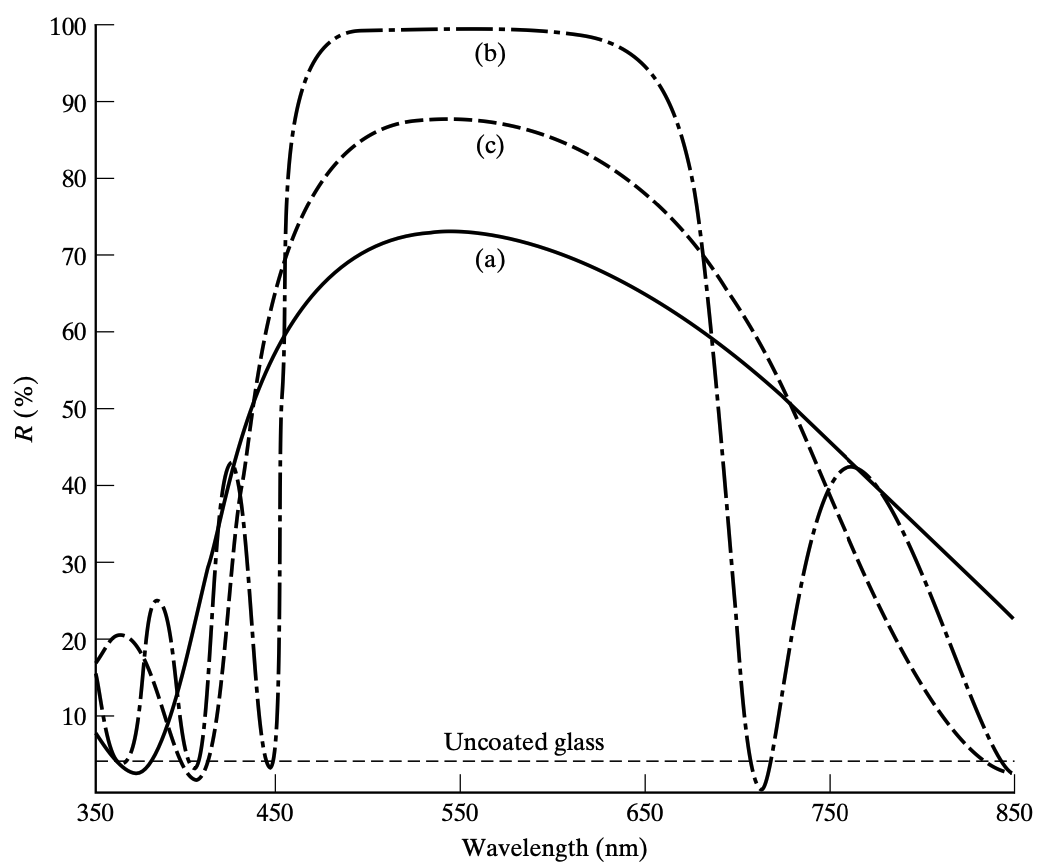
\includegraphics[width=\textwidth]{Chapters/Figures/Chapter 4 Figures/High-Reflectance Graphs in the Optics Book.png}
    \caption{Reflectance spectra for high-low index stacks: (a) for a two-layer double stack, (b) for a six-layer double stack, and (c) for a two-layer double stack enhanced with an additional high-index layer at the very top. Source: \cite{pedrotti_introduction_2007}}
    \label{fig:Reflectance spectra from optical literature}
  \end{minipage}\hfill
  % Right figure
  \begin{minipage}{0.48\textwidth}
    \centering
    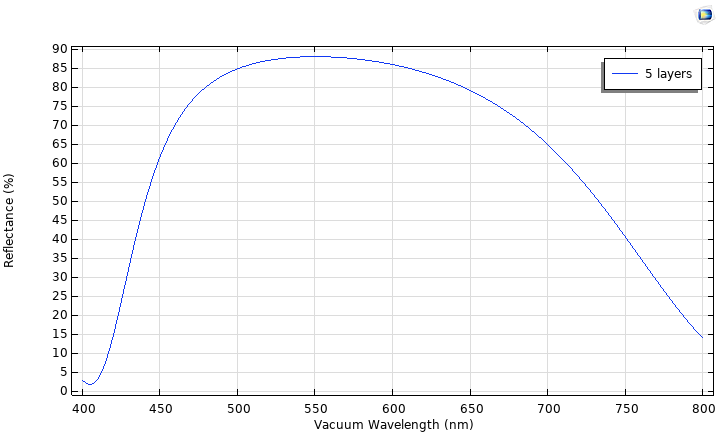
\includegraphics[width=\textwidth]{Chapters/Figures/Chapter 4 Figures/High-Reflectance (5 Layers).png}
    \caption{Spectral reflectance for a structure with two pairs of high-low refractive index layers, topped with an additional high-index layer. This figure is similar to plot (c) present in the left figure.}
    \label{fig:Reflectance 5-layer structure}
  \end{minipage}
\end{figure}

In these configurations, layers are designed to be $\lambda/4$ thick at a design wavelength $\lambda_0 = 550$ nm. Here, the high-index material (Zinc Sulfide - ZnS) has $n_H = 2.35$, the low-index material (Magnesium Fluoride - $\text{MgF}_2$) has $n_L = 1.38$, and the incident medium (air) has $n_0 = 1.00$. The ratio of $\frac{n_L}{n_H}$ is thus approximately $\frac{1.38}{2.35} \approx 0.587$.

Our analysis will specifically address graph (c), which demonstrates how adding an extra high-index layer between the substrate and the final low-index layer enhances maximum reflectance in a two-layer double stack ($N = 2$). This addition improves reflectance efficiency compared to simpler two-layer double configurations.

The findings showcased below stem from applying the high reflectance principles discussed in Chapter 2.

Observe the alignment of peak reflectance with the textbook's findings, achieving 90\%.

Employing a parametric sweep in COMSOL allows for the exploration of reflectance variation across wavelengths by systematically adjusting the count of double layer pairs ($N$) to values such as 2, 5, 10, and 20. This approach calculates solutions across a range of parameter sets. For all depicted graphs, an extra top layer with a high refractive index is incorporated to broaden the spectrum of maximum reflectance.

\begin{figure}[H]
  \centering
  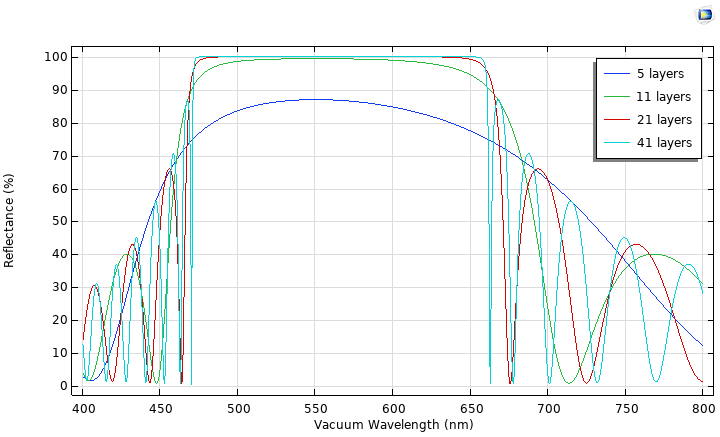
\includegraphics[width=0.7\textwidth]{Chapters/Figures/Chapter 4 Figures/High-Reflectance (5, 11, 21, and 41 Layers).png}
  \caption{Reflectance comparison for configurations with 5, 11, 21, and 41 layers, each enhanced by an additional high-index surface layer.}
  \label{fig:COMSOL multi-layer reflectance results}
\end{figure}

Unlike conventional metallic mirrors, DBRs leverage a careful and simple engineered structure of alternating thin layers of materials with contrasting refractive indices. This design typically features an odd number of layers, anchored by high refractive index materials at both ends, optimizing their reflectivity \cite{multiphysics__distributed_nodate}.

At the core of a DBR's functionality is the concept of constructive interference. As optical waves encounter the boundaries between layers, each boundary induces a partial reflection. When the optical wave's wavelength is four times the layers' optical thickness, these reflections interfere constructively, transforming the layers into an efficient reflector. This principle gives rise to a \emph{stopband}, a wavelength range where the reflector achieves heightened reflection. With an adequate number of layers, a DBR can achieve a high-quality reflection, making it useful in the operation of vertical cavity surface emitting lasers \cite{multiphysics__distributed_nodate}.

Expanding beyond the \emph{stopband}, DBRs exhibit a characteristic where reflectance transitions into a pattern of oscillating maxima and minima. By strategically adjusting these parameters, it is possible to shift the stopband's center, enhancing the filter's spectral transmittance across a broader range. This capability to finely control the light's passage through these structures not only underscores the versatility of DBRs but also paves the way for their integration into a wide array of optical devices, where precise manipulation of light is paramount \cite{pedrotti_introduction_2007}.

% ----- SECTION: COMSOL: MODELING PDRCs -----

\section{COMSOL: Modeling PDRCs}
At Hudgings Lab, one of the foundational PDRC designs comprises a straightforward sequence of layers. Beginning with silicon as the foundation, a layer of silver is applied directly above, topped with a final layer of Polydimethylsiloxane (PDMS).

\begin{figure}[H]
  \centering
  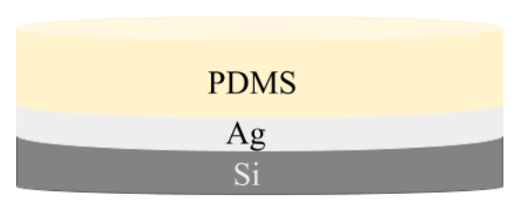
\includegraphics[width=0.7\textwidth]{Chapters/Figures/Chapter 4 Figures/PDRC Layout.png}
  \caption{Illustration of a basic PDRC configuration at Hudgings Lab, featuring a silicon base with subsequent layers of silver and PDMS.}
  \label{fig:PDRC-configuration-Hudgings-Lab}
\end{figure}

To understand the optical behavior of this structure, I systematically approached the modeling process from the bottom layer upwards. The following results present a sequence of reflectance versus wavelength analyses for each layer configuration: initially for silicon, followed by silicon with an added silver layer, and concluding with the composite structure of silicon, silver, and PDMS. This progression illustrates how each layer contributes to the overall reflectance spectrum.

% ----- SUBSECTION: ANALYSIS OF SILICON LAYER ONLY -----

\subsection{Analysis of Silicon Layer Only}

\begin{figure}[H]
  \centering
  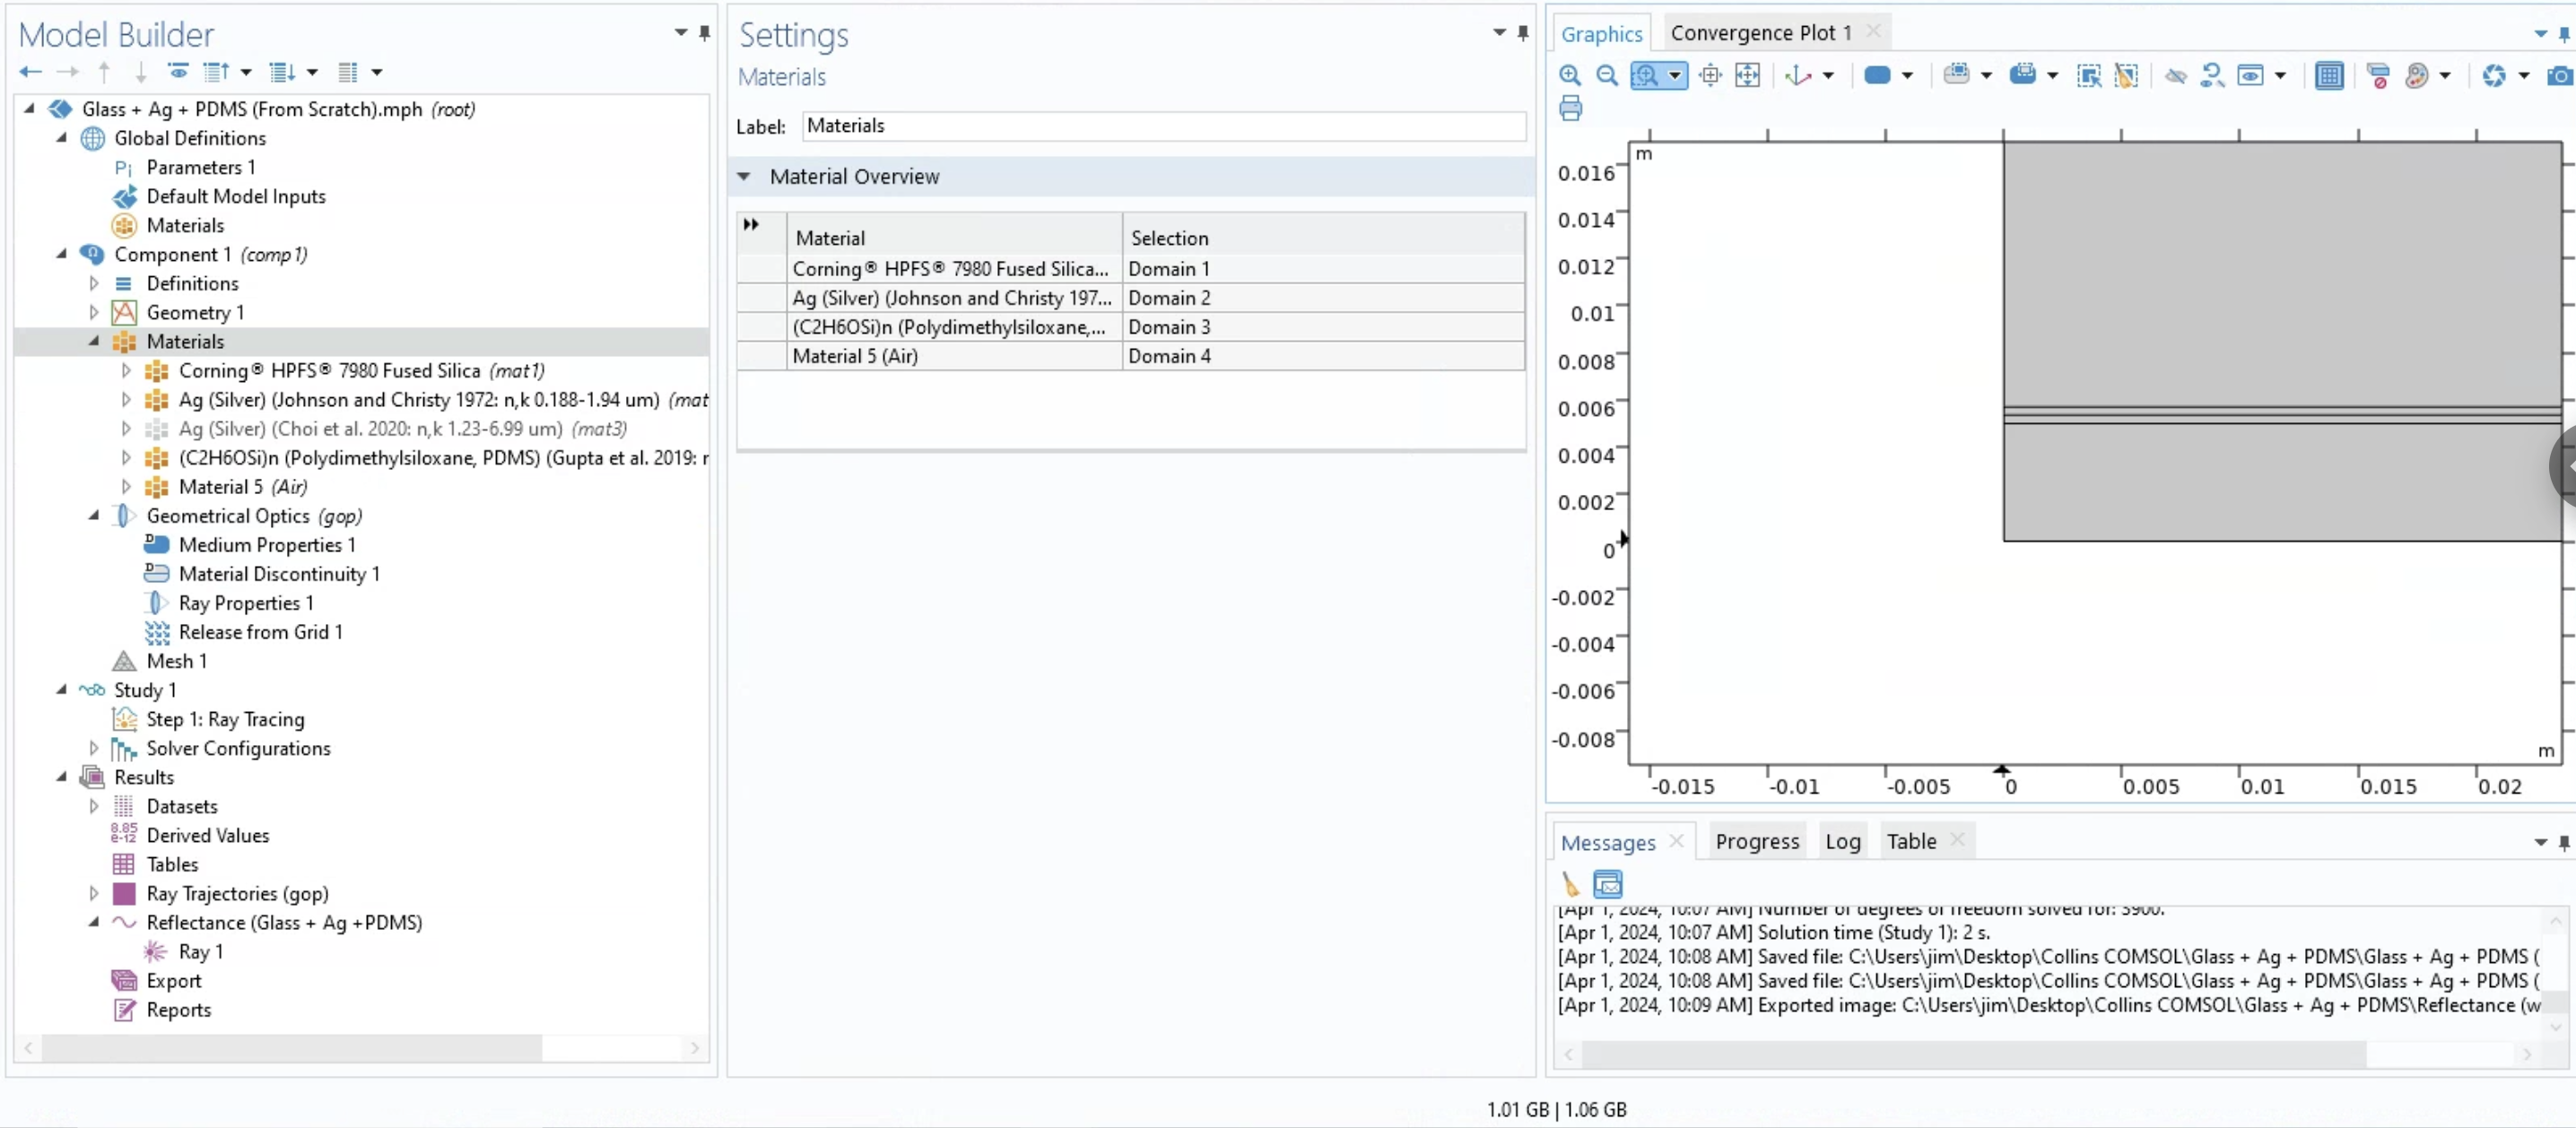
\includegraphics[width=0.7\textwidth]{Chapters/Figures/Chapter 4 Figures/COMSOL Desktop Layout for PDRC Analysis.png}
  \caption{COMSOL desktop setup for PDRC analysis demonstrating the simulation framework.}
  \label{fig:COMSOL-desktop-PDRC-setup}
\end{figure}

For simulations that span across various wavelengths, it is crucial to include the wavelength-dependence of the refractive indices of our materials. COMSOL tabulates $n(\lambda)$ for specific $\lambda$ measured in the literature. Then it interpolates between these experimentally measured points. This method allows for dynamic adjustment of a material's refractive index in response to changes in wavelength during simulations, providing a more accurate representation of the material's optical behavior.

\begin{figure}[H]
  \centering
  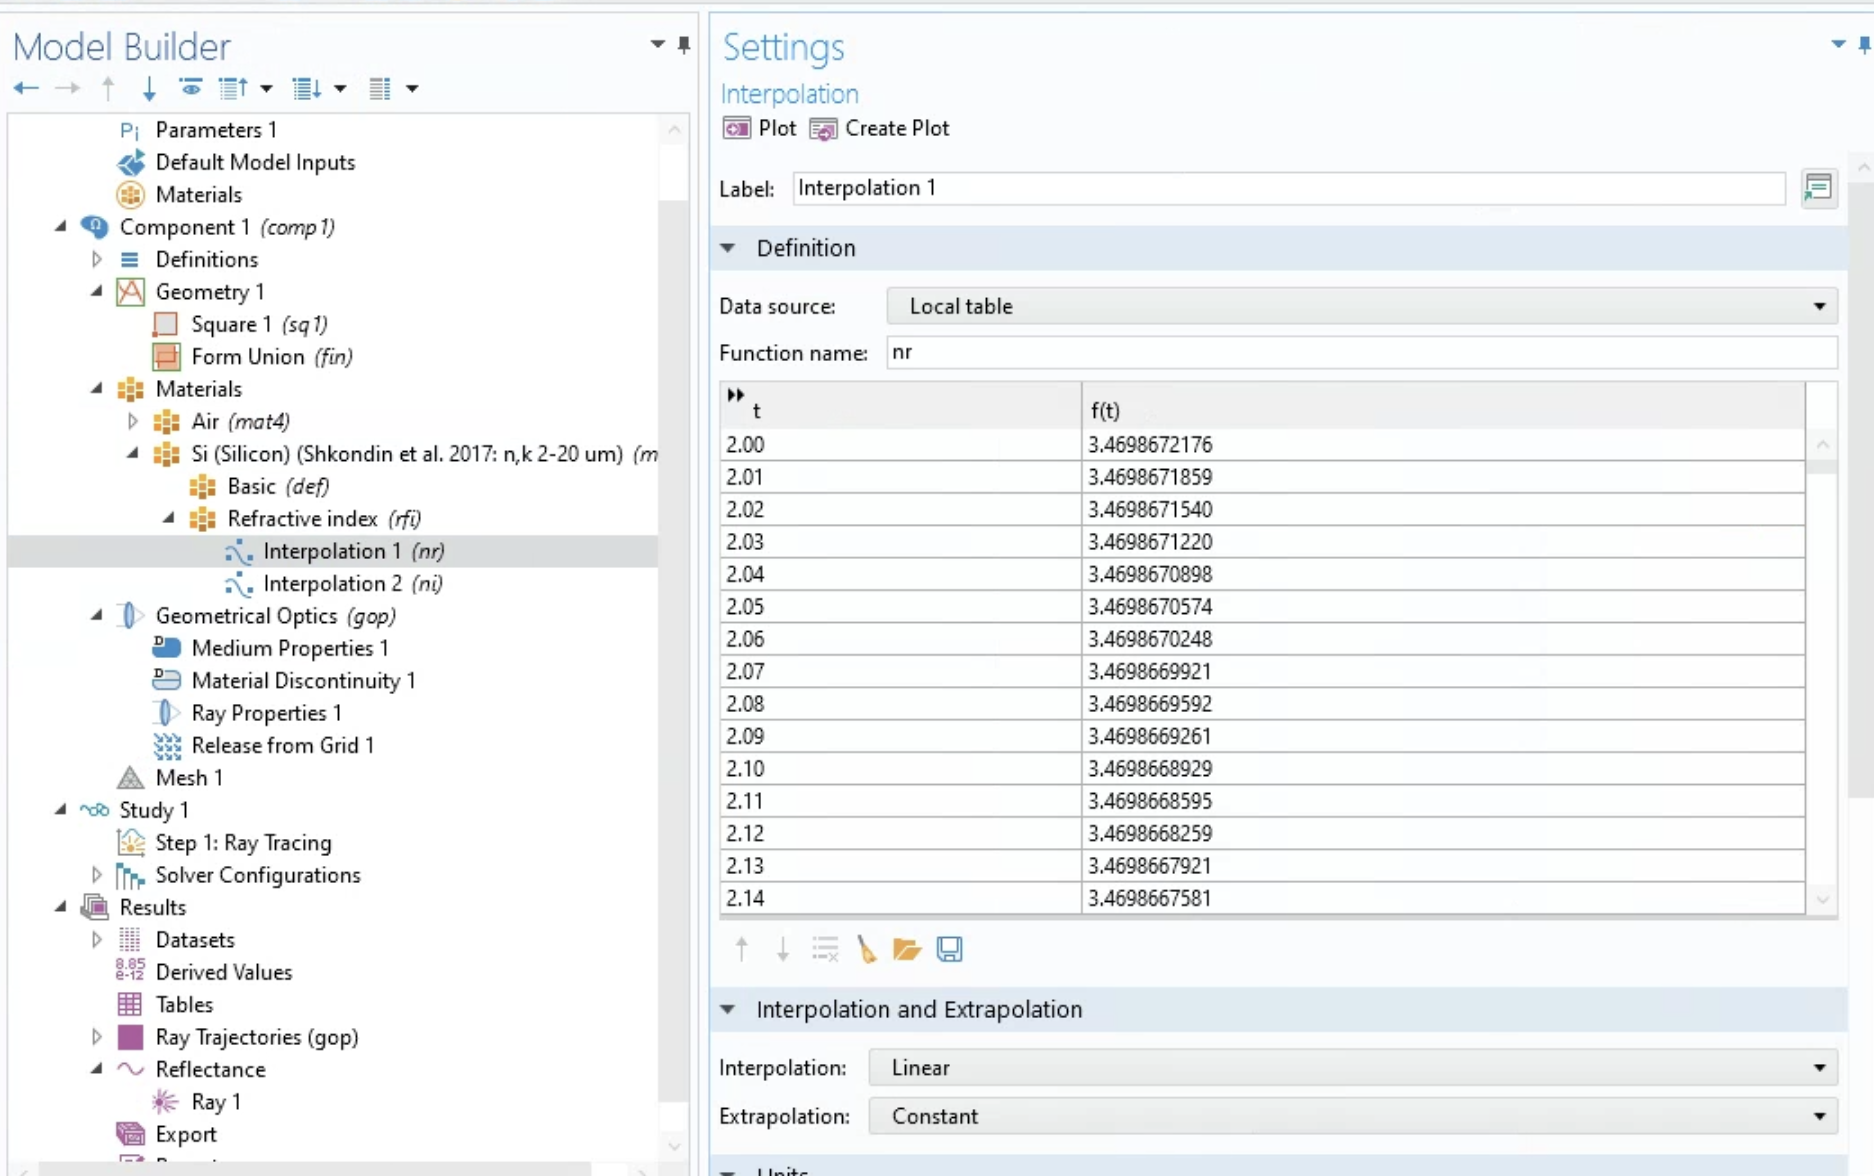
\includegraphics[width=0.7\textwidth]{Chapters/Figures/Chapter 4 Figures/Interpolation Table for the Silicon Substrate.png}
  \caption{Interpolation table for the silicon substrate, showing the wavelength-dependent refractive index.}
  \label{fig:interpolation-table-silicon}
\end{figure}

Utilizing the interpolation table enables the plotting of an interpolation function, offering a graphical representation of how refractive indices fluctuate with wavelength. This capability enriches the COMSOL simulation by providing a more precise depiction of light-material interaction over diverse wavelengths, a critical aspect in optics where dispersive phenomena play an important role.

% TODO: Add the interpolation plot for the silicon substrate
\begin{figure}[H]
  \centering
  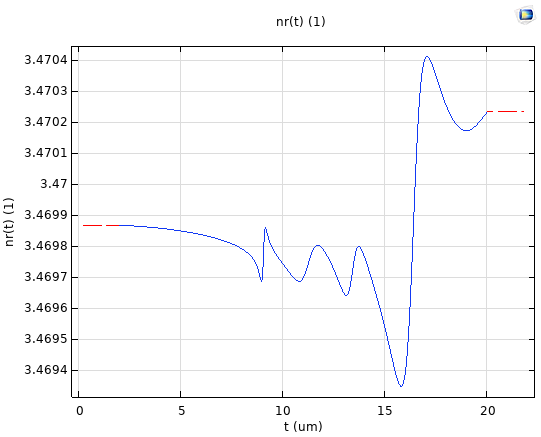
\includegraphics[width=0.7\textwidth]{Chapters/Figures/Chapter 4 Figures/Interpolation Plot (Silicon Substrate).png}
  \caption{Interpolation plot for the silicon substrate, showing the wavelength-dependent refractive index.}
  \label{fig:interpolation-plot-silicon}
\end{figure}

For this reason, I selected \emph{(Silicon) (Shkondin et al. 2017: n,k 2-20 um)} for the substrate, taking advantage of its accompanying interpolation function. It is vital to acknowledge that interpolation functions, which depict the wavelength-dependent refractive index variations of materials, can also be derived from experimental data found in scientific literature.

When generating a reflectance versus wavelength graph using only the silicon substrate, the reflectance indeed shows variation across different wavelengths.

\begin{figure}[H]
  \centering
  % Left image
  \begin{minipage}{0.48\textwidth}
    \centering
    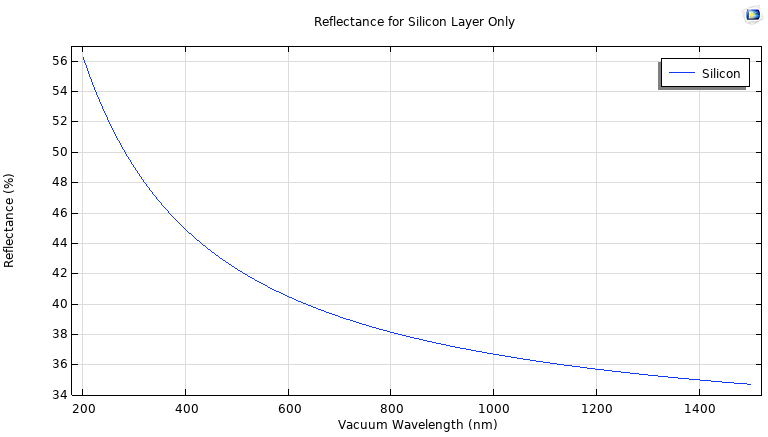
\includegraphics[width=\textwidth]{Chapters/Figures/Chapter 4 Figures/Reflectance (SIlicon Substrate Only).png}
    \caption{Reflectance variation with wavelength for \emph{(Silicon) (Shkondin et al. 2017: n,k 2-20 um)}.}
    \label{fig:Reflectance-Silicon-Substrate}
  \end{minipage}\hfill
  % Right image
  \begin{minipage}{0.48\textwidth}
    \centering
    \includegraphics[width=\textwidth]{Chapters/Figures/Chapter 4 Figures/Just Silicon (Fernando's Results).png}
    \caption{Reflectance variation with wavelength for Silicon, as experimentally determined by Fernando Castillo from Hudgings Lab. The reflectance measurements were conducted at an angle of 10 degrees from the normal.}
    \label{fig:Reflectance-Fernando-Results}
  \end{minipage}
\end{figure}

Within the displayed wavelength range, a sole substrate yields a reflectance below  45\% within the visible spectrum, which falls short of the desired high reflectivity within the solar spectrum for optimal PDRC performance. This observation underscores the need for integrating materials capable of meeting the dual objectives of high solar reflectance and substantial emissivity within the atmospheric window.

Focusing initially on enhancing solar reflectance, designs at Hudgings Lab incorporate silver on top the substrate due to its exceptional reflectivity in the solar spectrum. Having illustrated the outcomes with merely the glass substrate and underscored the importance of a highly reflective layer in the solar spectrum, I will venture into simulating the combined effects of glass and silver layers.

% ----- SUBSECTION: ANALYSIS OF SILICON PLUS SILVER LAYERS -----

\subsection{Analysis of Silicon plus Silver Layers}
Next, I added a silver layer on top the silicon substrate, recognizing the continued necessity for an interpolation function to accurately represent silver's refractive index across various wavelengths.

COMSOL offers a comprehensive collection of silver materials, each accompanied by interpolation tables that chart the refractive indices over preferred wavelength spans. The entry \emph{Ag (Silver) (Ciesielski et al. 2017: Ag/SiO2; n,k 0.191-20.9 um)} provides data on silver’s refractive indices from 0.191 to 20.9 ($\mu$m), where $n$ is the real component of the complex refractive index and $k$, the extinction coefficient, is the imaginary part, indicating the material's degree of light absorption.

\begin{figure}[H]
  \centering
  \includegraphics[width=0.7\textwidth]{Chapters/Figures/Chapter 4 Figures/Interpolation Table for Silver.png}
  \caption{Interpolation table for silver's refractive index.}
  \label{fig:Interpolation table for silver's refractive index}
\end{figure}

The figure below displays a plot of the refractive index interpolation of \emph{Ag (Silver) (Ciesielski et al. 2017: Ag/SiO2; n,k 0.191-20.9 um)}.

\begin{figure}[H]
  \centering
  \includegraphics[width=0.7\textwidth]{Chapters/Figures/Chapter 4 Figures/Interpolation Plot (Silver).png}
  \caption{Interpolation plot for silver's refractive index.}
  \label{fig:Interpolation plot for silver's refractive index}
\end{figure}

The figures below display the reflectance outcomes utilizing \emph{Ag (Silver) (Ciesielski et al. 2017: Ag/SiO2; n,k 0.191-20.9 um)}.

\begin{figure}[H]
  \centering
  % Left image
  \begin{minipage}{0.48\textwidth}
    \centering
    \includegraphics[width=\textwidth]{Chapters/Figures/Chapter 4 Figures/Silicon+Silver (Final Result).png}
    \caption{Reflectance results for Silicon and Silver Layers}
    \label{fig:Reflectance-Silicon-Silver}
  \end{minipage}\hfill
  % Right image
  \begin{minipage}{0.48\textwidth}
    \centering
    \includegraphics[width=\textwidth]{Chapters/Figures/Chapter 4 Figures/Silicon+Silver (Fernando's Results).png}
    \caption{Reflectance variation with wavelength for silicon and silver layers, as experimentally determined by Fernando Castillo. The reflectance measurements were conducted at an angle of 10 degrees from the normal.}
    \label{fig:Reflectance-Fernando-Results-Si-Ag}
  \end{minipage}
\end{figure}

These graphs mostly reflect the expected outcomes. Given silver's high reflectivity across the visible wavelength spectrum, we observe near 100\% reflectance within the visible range (400 - 700 nm).

% ----- SUBSECTION: ANALYSIS OF SILICON PLUS SILVER PLUS PDMS LAYERS -----

\subsection{Analysis of Silicon plus Silver plus PDMS Layers.}
In the final step, a PDMS layer was applied on top of the silver layer. This step also utilized a PDMS material equipped with a pre-defined interpolation function for its refractive index, specifically \emph{(C2H6OSi)n (Polydimethylsiloxane, PDMS) (Gupta et al. 2019: n 0.30-1.69 um)}.

\begin{figure}[H]
  \centering
  \includegraphics[width=0.7\textwidth]{Chapters/Figures/Chapter 4 Figures/Reflectance Results (Glass + Ag + PDMS).png}
  \caption{Reflectance analysis for a composite of glass, silver, and PDMS.}
  \label{fig:Reflectance analysis for glass, silver, and PDMS}
\end{figure}

This configuration resulted in reflectance maintaining a peak at 100\% across an extensive range of wavelengths.


---


We conclude our examination of optical phenomena using COMSOL. This chapter had two aims: first, to validate theoretical concepts like anti-reflectivity and high reflectance using COMSOL, and second, to initiate the simulation of basic PDRC configurations as designed at Hudgings Lab.

We began by evaluating anti-reflective strategies, ranging from simple to complex multilayer systems, against theoretical predictions from \emph{Introduction to Optics} by Frank L. Pedrotti et al. This comparison affirmed the accuracy of our simulations. Additionally, we modeled PDRC devices by layering glass, silver, and Polydimethylsiloxane (PDMS), revealing key optical properties essential for passive cooling effectiveness.

This chapter demonstrates the synergy between theoretical physics and computational modeling, offering a solid foundation for future research to expand upon. It underscores the importance of simulation in confirming theoretical models and opens avenues for improving PDRC device design.

Looking forward, the results from this chapter not only validate our understanding of optical principles but also suggest strategies for enhancing PDRC performance through material and design optimization.

\chapter{Conclusion}
The initial chapters laid the groundwork by illustrating the critical role of cooling technologies in addressing the pressing issues of global warming and the energy crisis. With an emphasis on PDRCs, we embarked on a journey through the theoretical underpinnings and practical applications of these devices, which offer the potential for efficient, energy-free cooling by radiating heat directly to outer space during daylight hours.

Throughout this exploration, we leveraged the capabilities of COMSOL Multiphysics™ to simulate various PDRC configurations, aiming to enhance their performance by optimizing material properties and layering strategies. The results chapter validated our approach, demonstrating the effectiveness of PDRCs in achieving significant cooling effects under real-world conditions.

As we culminate this research, this concluding chapter aims to distill the insights gained from our investigations, outlining the contributions of this work to the field of cooling technologies and the broader context of sustainable energy solutions.

\section{Our work}

COMSOL Multiphysics \texttrademark \space has proven itself as an indispensable tool for computational modeling, facilitating the simulation of intricate PDRC structures with relative ease. The modeling approach, exemplified in Chapter 3 through a detailed walkthrough with a busbar example, laid the foundation for all subsequent simulations.

This thesis has not only corroborated established theoretical principles within the realms of anti-reflectivity and high reflectance but has also ventured into the modeling of Fresnel equations to observe the behavior of reflection coefficients across varying angles of incidence.

The core of our efforts was the computational modeling of PDRC designs from Hudgings Lab, layer by layer, revealing critical insights into their optical performance. Notably, the simulation results confirmed the imperative for PDRCs to exhibit high reflectivity within the solar spectrum, a requirement clearly illustrated by the limited reflectivity observed in the sole glass substrate model.

\section{Future Directions}

Moving forward, several avenues for further research have been identified:

\begin{enumerate}
    \item Enhanced definition in the reflectance versus wavelength graphs for glass plus silver and glass plus silver plus PDMS models, possibly through the utilization of more detailed refractive index interpolation tables or functions.
    \item Exploration of adding more materials on top of the PDMS layer to fulfill PDRC design criteria more effectively, experimenting with various thicknesses and refractive indices to exploit constructive interference across multiple interfaces more efficiently.
    \item The translation of computational models into physical prototypes for empirical validation in lab settings, comparing simulated reflectance with real-world performance.
    \item Development of reflectance versus angle of incidence models to aid in the characterization of PDRC behavior throughout the day, providing a benchmark for experimental testing on rooftop installations.
\end{enumerate}

\section{Final Remarks}

This thesis not only validates the utility of PDRCs within the context of sustainable cooling technologies but also charts a course for their further development and application especially on the computational modeling front.

As we look to the future, the insights and methodologies presented here will serve as a valuable resource for those endeavoring to advance the efficiency and applicability of PDRCs and similar technologies in our collective pursuit of environmental sustainability and energy efficiency.

% the \appendix tag tells LaTeX where it should start labeling chapters with letters (denoting appendices) rather than numbers (denoting main chapters)
\appendix 


\chapter{An appendix}
% Look!  An Appendix!




% \bibliographystyle tells LaTeX how you want to format your bibliography.  There are many standard formats.  apsrev is fairly typical, but feel free to explore other options if the mood strikes.  
\bibliographystyle{apsrev}

% \bibliography calls the actual file that contains your bibliographic information.  This file can be generated by hand or in an automated way using software such as BibTeX.  Either works fine, but it is worth learning to use BibTex in the long term.  Take a look at the .bib file included here if you want to get some idea of the formatting required to create a bibliogrphy file of your own.

\bibliography{bibliography}
\end{document}